\documentclass[11pt]{article}
\usepackage[T1]{fontenc}
\usepackage[utf8]{inputenc}
\usepackage{lmodern}
\usepackage[a4paper,margin=28mm]{geometry}
\usepackage{amsmath,amssymb,amsthm,mathtools,bm}
\usepackage{enumitem}
\usepackage{microtype}
\usepackage{needspace}
\usepackage{xcolor}
\usepackage{tikz}
\usetikzlibrary{arrows.meta}
\usepackage[numbers,sort&compress]{natbib}
\PassOptionsToPackage{hyphens}{url}
\usepackage{hyperref}
\usepackage[nameinlink,noabbrev]{cleveref}
\hypersetup{colorlinks=true,linkcolor=blue!45!black,citecolor=blue!45!black,urlcolor=blue!45!black,
  pdftitle={Gigli's distributional curvature characterization of Alexandrov spaces},
  pdfauthor={OpenAI},
  pdfsubject={Gigli's characterization conjecture in dimensions at least two}}
\setlength{\emergencystretch}{2em}
\setlist[enumerate]{label=\textup{(\roman*)},leftmargin=2.2em}
\setlist[itemize]{leftmargin=1.8em}
\numberwithin{equation}{section}
\newtheorem{theorem}{Theorem}[section]
\newtheorem{lemma}[theorem]{Lemma}
\newtheorem{proposition}[theorem]{Proposition}
\newtheorem{corollary}[theorem]{Corollary}
\theoremstyle{definition}
\newtheorem{definition}[theorem]{Definition}
\theoremstyle{remark}
\newtheorem{remark}[theorem]{Remark}
\AddToHook{env/theorem/before}{\Needspace{3\baselineskip}}
\AddToHook{env/lemma/before}{\Needspace{3\baselineskip}}
\AddToHook{env/proposition/before}{\Needspace{3\baselineskip}}
\AddToHook{env/corollary/before}{\Needspace{3\baselineskip}}
\AddToHook{env/definition/before}{\Needspace{3\baselineskip}}
\AddToHook{env/remark/before}{\Needspace{3\baselineskip}}
\crefname{theorem}{Theorem}{Theorems}
\crefname{lemma}{Lemma}{Lemmas}
\crefname{proposition}{Proposition}{Propositions}
\crefname{corollary}{Corollary}{Corollaries}
\crefname{definition}{Definition}{Definitions}
\crefname{remark}{Remark}{Remarks}
\crefname{section}{Section}{Sections}
\crefname{equation}{Equation}{Equations}
\newcommand{\RCD}{\mathrm{RCD}}
\newcommand{\CD}{\mathrm{CD}}
\newcommand{\CBB}{\mathrm{CBB}}
\newcommand{\Test}{\operatorname{Test}}
\newcommand{\TestV}{\operatorname{TestV}}
\newcommand{\Hess}{\operatorname{Hess}}
\newcommand{\Ent}{\operatorname{Ent}}
\newcommand{\R}{\mathbb R}
\newcommand{\N}{\mathbb N}
\DeclareMathOperator{\Lip}{Lip}
\DeclareMathOperator{\supp}{supp}
\renewcommand{\Cap}{\operatorname{Cap}}
\DeclareMathOperator{\Geo}{Geo}
\DeclareMathOperator{\divg}{div}
\newcommand{\dd}{\,\mathrm d}
\newcommand{\weakto}{\rightharpoonup}
\newcommand{\eps}{\varepsilon}
\newcommand{\sk}{\mathfrak s_\kappa}
\newcommand{\ck}{\mathfrak s'_\kappa}
\allowdisplaybreaks[2]

\makeatletter
\renewcommand{\maketitle}{%
  \begin{center}
    {\Large\@title\par}
    \vspace{.4em}
    {\normalsize\@author\par}
    \vspace{.25em}
    {\small\@date\par}
  \end{center}}
\makeatother
\renewcommand{\bibsection}{%
  \section*{\refname}%
  \addcontentsline{toc}{section}{\refname}}

\title{Gigli's distributional curvature\\characterization of Alexandrov spaces}
\author{OpenAI}
\date{September 24, 2026}
\begin{document}
\maketitle
\begin{abstract}
For every integer \(n\ge2\) and \(\kappa\in\mathbb R\), we prove that
a complete separable metric space is an \(n\)-dimensional Alexandrov
space of curvature at least \(\kappa\) if and only if, with reference
measure \(\mathcal H^n\), it is a full-support
\(\RCD((n-1)\kappa,n)\) space whose distributional sectional curvature
is at least \(\kappa\) in Gigli's original global test classes.
This resolves Gigli's characterization conjecture in dimensions at least two.
\end{abstract}
{\small\tableofcontents}
\clearpage
\section{Introduction}
\label{sec:introduction}

On a smooth Riemannian manifold, a lower bound for sectional curvature
is equivalent to a lower comparison bound for geodesic triangles.
Gigli's distributional curvature tensor makes the analytic side of
this statement meaningful on spaces with synthetic lower Ricci
curvature bounds. The purpose of this paper is to prove that the same
equivalence holds in that setting, with the Hausdorff measure and
dimension hypotheses proposed by Gigli.



An Alexandrov lower curvature bound \(\CBB(\kappa)\) means that
geodesic triangles satisfy lower comparison with the simply connected
surface of constant curvature \(\kappa\), at the usual model scale
when \(\kappa>0\). A \(\RCD(K,N)\) space combines the
unreduced optimal-transport curvature-dimension condition
\(\CD(K,N)\) with quadratic Cheeger energy. The latter gives a
Hilbertian Sobolev calculus in which the tensor below is defined.
We take the reference measure to be the exact Hausdorff measure,
not merely a measure equivalent to it.

On a full-support finite-dimensional \(\RCD\) space \((M,d,m)\),
we use the nonpositive Laplacian:
\[
\int_M\langle\nabla f,\nabla h\rangle\dd m
=-\int_M(\Delta f)h\dd m.
\]
The domain \(D(\Delta)\) is the domain of the \(L^2\) generator.
In particular, its members belong to \(W^{1,2}(M)\). Our test classes are
\begin{align}
\label{eq:test-class}
\Test(M)
&=\left\{f\in D(\Delta):
\begin{array}{l}f\text{ has a bounded globally Lipschitz representative},\\
\Delta f\in W^{1,2}(M)
\end{array}\right\},\\
\label{eq:test-vector-class}
\TestV(M)
&=\left\{\sum_{j=1}^{\ell}a_j\nabla b_j:
\ell<\infty,\ a_j,b_j\in\Test(M)\right\}.
\end{align}
For test fields set
\([X,Y]=\nabla_XY-\nabla_YX\), where \(\nabla\) is the weak
Levi--Civita covariant derivative. The curvature functional is
\begin{align}
\label{eq:curvature-definition}
R(X,Y,Z,W)(f)=\int_M&
-\langle\nabla_X(fW),\nabla_YZ\rangle
-f\langle\nabla_YZ,W\rangle\divg X \notag\\
&+\langle\nabla_Y(fW),\nabla_XZ\rangle
+f\langle\nabla_XZ,W\rangle\divg Y \notag\\
&-f\langle\nabla_{[X,Y]}Z,W\rangle\dd m.
\end{align}
The last derivative means contraction of the weak derivative of \(Z\)
with \([X,Y]\). This is the sign convention corresponding to
\(\nabla_X\nabla_Y-\nabla_Y\nabla_X-\nabla_{[X,Y]}\).
All terms in \eqref{eq:curvature-definition} are integrable in the
test classes \eqref{eq:test-class}--\eqref{eq:test-vector-class}.
No classical curvature tensor is assumed.

\begin{theorem}[Gigli's characterization]
\label{main:equivalence}
Let \(n\ge2\) be an integer, let \(\kappa\in\R\), and let \((M,d)\)
be a complete separable metric space. The following conditions are
equivalent.
\begin{enumerate}[label=\textup{(\Alph*)}]
\item \((M,d)\) is an \(n\)-dimensional Alexandrov space with curvature
bounded below by \(\kappa\).
\item With \(m=\mathcal H^n_d\), the space \((M,d,m)\) has full support,
is \(\RCD((n-1)\kappa,n)\), and satisfies
\begin{equation}
\label{eq:main-curvature}
R(X,Y,Y,X)(f)\ge
\kappa\int_M f\bigl(|X|^2|Y|^2-\langle X,Y\rangle^2\bigr)\dd m
\end{equation}
for every \(X,Y\in\TestV(M)\) and every nonnegative \(f\in\Test(M)\).
\end{enumerate}
The \(\RCD\) condition is unreduced, and the test classes and
curvature sign are exactly those defined above.
\end{theorem}

\subsection{History and significance}

Lott--Villani and Sturm independently developed synthetic lower
Ricci curvature bounds through convexity properties of entropy along
Wasserstein geodesics \cite{LottVillani2009,Sturm2006I,Sturm2006II}.
Ambrosio--Gigli--Savar\'e introduced the \(\RCD(K,\infty)\)
framework, imposing quadratic Cheeger energy to select a Riemannian
class \cite{AGS2014}. Ambrosio--Gigli--Mondino--Rajala extended
the theory to reference measures finite on bounded sets and removed
the strengthened entropy condition in the original definition
\cite{AGMR2015}. These developments supply the ambient Ricci-curvature
and Sobolev framework for the sectional-curvature question considered here.

Petrunin and Zhang--Zhu established the connection between
Alexandrov lower curvature bounds and the curvature-dimension condition
\cite{Petrunin2011,ZhangZhu2010}.
The quadratic Sobolev theory of Kuwae--Machigashira--Shioya
\cite{KMS2001} supplies the Riemannian structure.
The full-scope Alexandrov-to-\(\RCD\) statement used below is recorded
in \cite[Theorem~2.9 and Corollary~2.10]{KapovitchKettererSturm}.
Gigli subsequently defined
\eqref{eq:curvature-definition} and conjectured the
characterization proved here in dimensions at least two
\cite[Conjecture~1.1]{Gigli2019}.
His construction gives tensor symmetries and tensoriality, but does
not by itself relate a lower tensor bound to triangle comparison.

Theorem~\ref{main:equivalence} resolves this conjecture positively
for every integer \(n\ge2\).
The exact choice of reference measure is important:
the assumption \(m=\mathcal H^n\) supplies noncollapsed structure,
including \(n\)-dimensional Euclidean tangents almost everywhere
\cite{DPG2018}.
The use of the original test classes is important as well.
The theorem is neither a statement about a classical tensor on a
regular subset nor a restriction to compactly supported fields.

Optimal transport also gives a characterization of sectional
curvature in the smooth setting. Ketterer--Mondino express sectional
and intermediate Ricci bounds through entropy inequalities along
Wasserstein geodesics supported on lower-dimensional rectifiable
sets \cite{KettererMondino2018}. The transport calculation here pairs
full-dimensional densities with Gigli's distributional tensor.

Several related developments locate the analytic difficulties.
Lebedeva--Petrunin construct a weak curvature tensor for smoothable
Alexandrov spaces, using noncollapsing smooth approximations with a
common sectional lower bound \cite{LebedevaPetrunin2024}. Their weak-limit
tensor is a separate framework from the global test-class functional
considered here.
Brena--Gigli studied measure representations of weak Hessians and
curvature tensors, and explained the regularity obstruction in
passing from a distributional Hessian bound to convexity
\cite[Remark~2.4 and Remark~2.18]{BrenaGigli2024}.
For \(C^1\) Riemannian metrics, Er\"os--Kunzinger--Ohanyan--Vardabasso
proved a local distributional-to-Alexandrov comparison result
\cite[Theorem~3.1]{EKOV2026}.
The argument here works directly with the Sobolev calculus of a
noncollapsed \(\RCD\) space.

\subsection{The new arguments}

Section~\ref{sec:forward} proves the forward implication.
The converse proceeds through the index inequality of
Theorem~\ref{heat:index}, the Hessian comparison of
Theorem~\ref{frames:hessian}, and the passage to comparison along
every geodesic in Section~\ref{sec:weighted-comparison}.

\paragraph{Integrated configurations.}
Section~\ref{sec:forward} extracts the curvature functional from
small Alexandrov configurations. The expansion is integrated against
transported densities. A quantitative first-order estimate for the
interpolating density permits pairing with fixed \(L^2\) Hessian
coefficients. The geometric comparison and the transport expansion
bound the same energy difference. Averaging cancels the lower-order
terms. Suitable endpoint corrections then identify the remaining
coefficient as the curvature term plus a nonnegative square error.
Local choices of gradient tests make this error arbitrarily small.
Tensoriality, approximation and exhaustion then
recover the global test classes in Theorem~\ref{fwd:curvature}.
The calculation uses only the weak derivatives provided by the test calculus.

\paragraph{A heat-regularized index inequality.}
Section~\ref{sec:heat-index} pairs a forward heat factor with a backward
heat factor normalized by the prescribed terminal density.
Their product solves a continuity equation. The logarithmic
potentials yield a Riccati identity, in which the terms containing
the inverse viscosity cancel. The remaining acceleration error must
be controlled uniformly up to the terminal time, including the
singular measure terms in the Bochner inequality. A one-sided
estimate supplies this control. An action identity gives strong convergence of
the velocities in the density-weighted norm, which is needed for
the quadratic index energy.

\paragraph{Frames through exceptional times.}
Almost-everywhere spatial regularity alone does not give a frame at
every time on a path. Section~\ref{sec:frames} upgrades harmonic
splitting maps to frames along almost every relevant entire path. A Hausdorff-content
estimate controls the regular points where a countable family of
test gradients fails to have full rank. Capacity estimates and
bounded-compression path estimates remove the exceptional sets.
Deng's continuity theorem for tangent cones along every geodesic
\cite{Deng2020} supplies regularity at all interior times.
Caputo--Gigli--Pasqualetto established parallel transport along test
plans in the noncollapsed setting \cite{CGP2022}. Here finite-dimensional
Sobolev ODEs in the selected frames construct and approximate the
Jacobi trials needed by the index inequality. Only a countable trial catalog
is needed; an integrated density theorem for parallel fields is not
assumed.

\paragraph{From Hessian comparison to every geodesic.}
Section~\ref{sec:weighted-comparison} constructs bounded global
modifications of the distance function. Their distributional Hessian
bounds fit the general theorem of the companion paper
\cite[Theorem~1.1]{WeakHessianCompanion}, recalled with its exact
hypotheses in Theorem~\ref{weight:every-geodesic}. That theorem applies
to every full-support \(\RCD(K,N)\) space with \(1<N<\infty\),
including collapsed spaces. Its proof uses bounded changes of measure
and a closed weighted Bochner inequality; it does not use the
characterization or the frame construction of this paper. Applied to
the modified distances, it gives the model differential inequality
along every minimizing geodesic. A one-dimensional comparison and
the local-to-global Alexandrov theorem finish the argument.

Figure~\ref{fig:proof-route} summarizes the reverse implication and
the point where the companion theorem is used.
\begin{figure}[t]
\centering
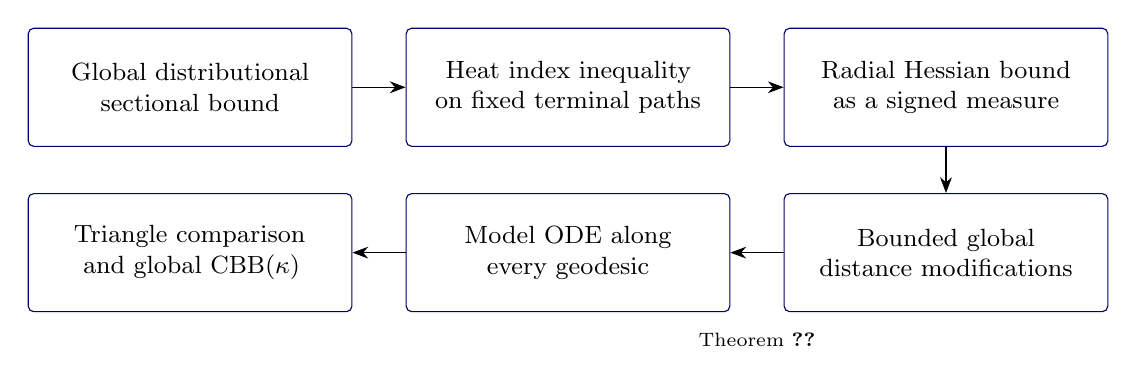
\begin{tikzpicture}[
 box/.style={draw=blue!40!black,rounded corners=2pt,align=center,
 text width=39mm,minimum height=15mm,font=\small,inner sep=3pt},
 >={Stealth[length=2mm]}]
\node[box] (tensor) at (0,0) {Global distributional\\sectional bound};
\node[box] (index) at (4.8,0) {Heat index inequality\\on fixed terminal paths};
\node[box] (hessian) at (9.6,0) {Radial Hessian bound\\as a signed measure};
\node[box] (distance) at (9.6,-2.1) {Bounded global\\distance modifications};
\node[box] (ode) at (4.8,-2.1) {Model ODE along\\every geodesic};
\node[box] (cbb) at (0,-2.1) {Triangle comparison\\and global $\CBB(\kappa)$};
\draw[->] (tensor) -- (index);
\draw[->] (index) -- (hessian);
\draw[->] (hessian) -- (distance);
\draw[->] (distance) -- node[below=9mm,font=\scriptsize,align=center]
 {Theorem~\ref{weight:every-geodesic}} (ode);
\draw[->] (ode) -- (cbb);
\end{tikzpicture}
\caption{The reverse implication. The noncollapsed frame and countable
trial construction connects the heat index estimate to the radial
Hessian bound. The companion theorem supplies the passage to every
geodesic after the bounded distance modification and has general
finite-dimensional RCD scope.}
\label{fig:proof-route}
\end{figure}


The frame and pathwise trial constructions in the first two
subsections of Section~\ref{sec:frames} also have an independent scope.
They apply on full-support noncollapsed \(\RCD(K,n)\) spaces,
with \(m=\mathcal H^n\) and integer \(n\ge2\), to optimal geodesic
plans with bounded positions, bounded speed and bounded compression
throughout the relevant interval. The approximation is pathwise,
using a countable catalog of global trials.

We state the foundational \(\RCD\) results in the form used in the
proof and give complete arguments for the additional transport,
index, frame and distance-comparison steps. The general reweighting
argument is supplied by the companion paper \cite{WeakHessianCompanion}.
Numbered external results refer to the source versions linked in
the bibliography; version notes specify differences from published
numbering where necessary.

\section{Calculus and background results}
\label{sec:preliminaries}

We collect the analytic conventions and the precise approximation
facts used below. Throughout this section \((M,d,m)\) is an
\(\RCD(K,N)\) space with \(N<\infty\), full support, and the
usual locally finite reference measure. All the analytic results
recalled here also hold under \(\RCD^*(K,N)\). We use them under the
unreduced hypothesis of Theorem~\ref{main:equivalence}.

\subsection{Test calculus and localization}

Besides \(\Test\), defined in \eqref{eq:test-class}, it is useful to
write
\[
\Test^\infty(M)=\{g\in\Test(M):\Delta g\in L^\infty(M)\}.
\]
The superscript refers to the additional Laplacian bound; it does
not mean classical smoothness. A function is a local test function
on an open set if it agrees on every relatively compact smaller
open set with a global test function. We write \(H_g\) for
\(\Hess g\), and identify the covector \(H_g(V,\cdot)\) with a
vector when using the notation \(H_gV\).

The following facts belong to the standard second-order
\(\RCD\) calculus \cite{Gigli2018,Gigli2019,Savare2014}.
Both test classes are algebras. A test function has an \(L^2\)
Hessian, and for test fields
\[
X\in L^2(TM)\cap L^\infty(TM),\qquad
\nabla X\in L^2(T^*M\otimes TM),\qquad
\divg X\in L^2(m).
\]
The connection is metric-compatible and torsion-free. In particular,
inner products of bounded test fields belong to \(W^{1,2}\),
and their differentials obey the usual product rule.
For gradients,
\[
\nabla_{\nabla g}\nabla g=\nabla\bigl(|\nabla g|^2/2\bigr).
\]
The curvature functional \eqref{eq:curvature-definition} has the
algebraic symmetries of Riemannian curvature and is tensorial over
\(\Test\), including
\begin{align}
\label{eq:curvature-symmetries}
R(X,Y,Z,W)&=-R(Y,X,Z,W)=R(Z,W,X,Y),\\
\label{eq:curvature-tensoriality}
R(aX,Y,Z,W)(f)&=R(X,Y,Z,W)(af)
\end{align}
for test functions \(a,f\), with the corresponding identity in every
slot \cite[Proposition~2.7]{Gigli2019}.

\begin{lemma}[Cutoffs and approximation]
\label{pre:approximation}
The following approximations are available.
\begin{enumerate}
\item For a compact set \(E\) in an open set \(U\), there is
\(\chi\in\Test^\infty\) with \(0\le\chi\le1\), equal to one on a
neighborhood of \(E\), and compactly supported in \(U\).
There are also exhausting cutoffs \(\chi_R\in\Test^\infty\),
equal to one on \(B_R(o)\), supported in \(B_{R+1}(o)\), whose
gradient and Laplacian bounds are independent of \(R\).
\item For \(g\in D(\Delta)\),
\begin{equation}
\label{eq:pre-hessian-estimate}
\|H_g\|_2^2\le
\|\Delta g\|_2^2+\max\{-K,0\}\|\nabla g\|_2^2.
\end{equation}
Compactly supported functions in \(\Test^\infty\) form a core
for \(\Delta\).
\item On a fixed compact region, a function \(g\in\Test\) can be
approximated by compactly supported \(g_j\in\Test^\infty\) with
uniformly bounded gradients, with
\[
g_j\to g,\qquad \nabla g_j\to\nabla g,\qquad
\Delta g_j\to\Delta g,\qquad H_{g_j}\to H_g
\quad\hbox{strongly in }L^2
\]
on that region.
\item A compactly supported Lipschitz function \(\xi\) can be
approximated by compactly supported test functions \(\xi_j\)
with a common compact support and a common Lipschitz bound,
uniformly and strongly in \(W^{1,2}\).
If \(\xi\ge0\), the approximants may be chosen nonnegative.
\end{enumerate}
\end{lemma}

\begin{proof}
The good-cutoff construction and the integrated Bochner estimate give
\textup{(i)} and \eqref{eq:pre-hessian-estimate}; see
\cite[Appendix~A, Lemma~A.2 and Equation~(A.13)]{GigliTamanini2021}.
For the local version of the cutoff construction one uses finitely
many small good cutoffs inside \(U\), and a smooth truncation of their
sum. This keeps the Laplacian bounded and Sobolev by the test
algebra and chain rules.

Let \(P_t\) denote the heat semigroup. For \(h\in L^2\cap L^\infty\),
positive-time regularization gives
\(P_th\in\Test^\infty\)
\cite[Appendix~A, Equation~(A.7)]{GigliTamanini2021}.
Spectral calculus and density of bounded \(L^2\) data show that these
regularizations form a core. For each such regularization \(h\),
\[
\Delta(\chi_Rh)
=\chi_R\Delta h+h\Delta\chi_R
+2\langle\nabla\chi_R,\nabla h\rangle.
\]
The uniform cutoff bounds and the \(L^2\) tails imply convergence
to \(\Delta h\) in \(L^2\), as well as convergence of the functions
and gradients. This proves the compact-core assertion.

For \textup{(iii)}, choose nested cutoffs \(\chi,\zeta\) such that
\(\chi=1\) near the region in question and \(\zeta=1\) near
\(\supp\chi\). Put
\[
g_t=\chi P_t(\zeta g).
\]
The function \(\zeta g\) lies in \(\Test\). The product rule,
spectral continuity and the fixed cutoff bounds give convergence
of \(g_t\) to \(\chi\zeta g\) in the Laplacian graph norm.
The Bakry gradient estimate gives
\[
\|\nabla g_t\|_\infty
\le \|\chi\|_\infty e^{-Kt}\|\nabla(\zeta g)\|_\infty
+\|\nabla\chi\|_\infty\|\zeta g\|_\infty.
\]
Apply \eqref{eq:pre-hessian-estimate} to
\(g_t-\chi\zeta g\) to obtain strong Hessian convergence.
Since \(\chi\zeta g=g\) near the region, \textup{(iii)} follows.

For \textup{(iv)}, use \(\xi_t=\chi P_t\xi\), with an outer
cutoff \(\chi=1\) near \(\supp\xi\).
The heat semigroup converges strongly in \(W^{1,2}\);
the uniform Lipschitz estimate and the small-time heat-kernel
moment bound give uniform convergence on the common compact
support. The cutoff product gives the same conclusions for
\(\xi_t\), and positivity is preserved.
\end{proof}

\begin{remark}
\label{pre:bare-gradients}
A compactly supported test gradient is a member of the global
\(\TestV\): multiply it by a test cutoff equal to one near its
support. This observation is necessary when \(m(M)=\infty\),
because the constant function one then need not lie in \(\Test\).
All uses of a bare test gradient below are local in this sense.
\end{remark}

\begin{lemma}[Lipschitz weights and continuity of the tensor]
\label{pre:tensor-continuity}
For fixed test fields the formula
\eqref{eq:curvature-definition} defines a functional on compactly
supported Lipschitz weights. It has the form
\[
f\longmapsto\int fA+\langle\nabla f,B\rangle\dd m,
\qquad A\in L^1_{\rm loc}(m),\quad B\in L^2_{\rm loc}(TM).
\]
It is continuous under the weight approximation in
Lemma~\ref{pre:approximation}\textup{(iv)}.
More generally, for weights with a common compact support,
uniform convergence of the weights and weak \(L^2\) convergence
of their gradients suffice.
The tensor identities remain valid for these weights.
Moreover, on a fixed compact set the functional is continuous
under uniformly bounded field approximations for which the fields,
their divergences and their covariant derivatives converge
strongly in \(L^2\), with the fields converging almost everywhere
along a subsequence.
\end{lemma}

\begin{proof}
Expand \(\nabla_X(fW)=X(f)W+f\nabla_XW\).
Every coefficient of \(f\) is a product of two \(L^2\) factors
and bounded factors. The coefficients of \(\nabla f\) lie in
\(L^2\). Uniform convergence of \(f_j\) pairs with the fixed
\(L^1\) coefficient, and weak \(L^2\) convergence of their
gradients pairs with the fixed \(L^2\) coefficient.
This proves the weight-continuity assertions.
Approximation then extends the identities.

For the field assertion,
\[
\nabla_{X_j}Y_j-\nabla_XY
=(\nabla Y_j-\nabla Y)(X_j)+\nabla Y(X_j-X).
\]
The first term tends to zero in \(L^2\) by uniform boundedness
of \(X_j\); the second does so by dominated convergence.
The brackets therefore converge in \(L^2\) as well.
Products of the resulting strongly convergent \(L^2\) quantities
converge in \(L^1\). Any remaining uniformly bounded field factor
is handled by almost-everywhere convergence and domination.
This includes the last term of
\eqref{eq:curvature-definition}.
\end{proof}

\subsection{Weak Hessians and Bochner measures}

For \(F\in W^{1,2}_{\mathrm{loc}}(M)\), a compact test gradient \(Y=\nabla g\),
and a compactly supported Lipschitz weight \(\xi\), define
\begin{equation}
\label{eq:weak-hessian}
H_F(Y,Y)(\xi)
=-\int_M\divg(\xi Y)\,\langle\nabla F,Y\rangle\dd m
-\int_M\xi\,\langle\nabla F,\nabla_YY\rangle\dd m.
\end{equation}
Polarization defines the mixed evaluation.
The two terms are integrable: \(\nabla F\), \(\divg(\xi Y)\)
and \(\nabla_YY\) are locally \(L^2\), and \(Y,\xi\) are bounded.
For fixed \(Y,\xi\), the functional is continuous under weak
local \(W^{1,2}\) convergence of \(F\).
When \(F\in D(\Delta)\), this agrees with the usual \(L^2\)
Hessian. A statement \(H_F(Y,Y)\le A\,m\) means the
corresponding inequality on every nonnegative compact Lipschitz
weight. It does not presuppose that \(H_F\) is an \(L^2\) tensor.

For a local test function \(g\), the measure-valued Bochner
inequalities are
\begin{align}
\label{eq:bochner-hessian}
\Gamma_2(g)
&:=\Delta\bigl(|\nabla g|^2/2\bigr)
-\langle\nabla g,\nabla\Delta g\rangle m
\ge \bigl(K|\nabla g|^2+|H_g|^2\bigr)m,\\
\label{eq:bochner-dimension}
\Gamma_2(g)&\ge
\bigl(K|\nabla g|^2+(\Delta g)^2/N\bigr)m.
\end{align}
Here the first Laplacian is a measure-valued Laplacian.
We use the two inequalities separately or after taking a convex
combination; no inequality with the sum of both squared terms
and coefficient one is asserted.
Our capacity normalization is
\[
\Cap_2(E)=
\inf_{\substack{U\supset E\\U\ \mathrm{open}}}
\ \inf_{\substack{v\in W^{1,2}(M)\\v\ge1\ m\text{-a.e.\ on }U}}
\int_M\bigl(v^2+|\nabla v|^2\bigr)\dd m.
\]
A polar set has zero \(2\)-capacity; \emph{quasi-everywhere} means
outside a polar set.
The Bochner measures do not charge sets of zero \(2\)-capacity.
Their Sobolev multipliers are evaluated using quasi-continuous
representatives \cite[Sections~2.3 and 3.2]{Savare2014}.

More explicitly, if bounded Sobolev multipliers converge strongly
in \(W^{1,2}\), with a common bound and compact support, a
subsequence converges outside a polar set. Dominated convergence
therefore applies to their integrals against each fixed local
Bochner measure. This extends the integration-by-parts identities
from test multipliers to bounded Sobolev multipliers.
The same argument shows that an almost-everywhere lower bound for
a Sobolev multiplier holds for its quasi-continuous representative
outside a polar set. These facts will be used when multiplying
singular Bochner measures in Section~\ref{sec:heat-index}.

The inequalities \eqref{eq:bochner-hessian}--\eqref{eq:bochner-dimension}
also hold for our original test class, without a bounded
Laplacian. One can see the extension locally by applying heat
regularization to a test function. The gradients remain uniformly
bounded, the Hessians converge strongly in \(L^2\), and
\(\nabla\Delta P_tg\to\nabla\Delta g\) in \(L^2\).
The local masses of the positive Bochner remainders are bounded
by testing with a fixed outer cutoff. Passage to the distributional
limit gives the asserted measure inequalities.

\subsection{Geometry, transport and along-curve calculus}

We use the following established facts, stating the restrictions
that are relevant to the proof.

\begin{enumerate}
\item A finite-dimensional full-support \(\RCD\) space is proper
and geodesic, is locally doubling, and satisfies a local
\(L^2\) Poincar\'e inequality and the Sobolev-to-Lipschitz property.
Bounded sets have finite measure. When the dimension parameter is
\(N=n\) and \(m=\mathcal H^n\), almost every point is \(n\)-regular and the
tangent module has dimension \(n\) almost everywhere. For every
bounded region and every fixed sufficiently small upper radius,
\begin{equation}
\label{eq:local-volume}
c\,r^n\le m(B_r(x))\le C\,r^n
\end{equation}
with positive constants uniform for centers in that region.
The upper bound is the noncollapsed density bound; the lower bound
follows from Bishop--Gromov and full support
\cite[Theorem~1.12 and Corollary~2.14]{DPG2018}.

\item Optimal quadratic transport between probability measures
\(\mu,\nu\in\mathcal P_2(M)\), with \(\mu\ll m\), is induced by
a unique dynamical map.
For a fixed real-valued \(c\)-concave potential, \(c=d^2/2\), the geodesic
from almost every point into its \(c\)-superdifferential is unique
\cite[Theorems~1.1 and 1.3]{GigliRajalaSturm2016}.
Between bounded densities with bounded support, the interpolating
densities are uniformly bounded and obey the pointwise
curvature-dimension distortion inequality.
We use the density bound also on subintervals with a singular
endpoint, whenever a separate positive-time compression estimate
has been proved. We do not assume bounded compression at a Dirac
endpoint.

\item A bounded-speed plan with bounded compression is a
Sobolev test plan. For a Sobolev function \(g\), its time
derivative is \(\langle\nabla g,v\rangle\), where \(v\) is the
plan velocity \cite[Theorem/Definition~2.33]{GigliDifferentialStructure}.
For a \(W_2\)-continuous curve with bounded compression, the
Sobolev continuity equation characterizes \(2\)-absolute
continuity and its action, and such curves have a superposition
by absolutely continuous metric paths
\cite[Theorem~3.5 and Proposition~2.1]{GigliHan2015}.
The required \(W_2\)-continuity is verified before using this
criterion in Section~\ref{sec:heat-index}.

\item For a bounded-support optimal geodesic test plan,
Gigli--Tamanini's second-order differentiation formula applies to
\(H^{2,2}\) functions and to vector-field pairings with
\(H_C^{1,2}(TM)\), the closure of \(\TestV(M)\) in the covariant
Sobolev norm \cite[Theorem~5.13]{GigliTamanini2021}.
Every vector field to which we apply this theorem is a compactly
supported test field.
It also applies after bounded measurable restriction of the
plan. This permits passage from integrated identities to
almost-sure time-distributional identities.

\item A compactly supported time-dependent test vector field,
bounded with bounded divergence and integrable Sobolev covariant
derivative, has the regular Lagrangian flow and uniqueness
properties used for the short flows below
\cite[Sections~8 and 9.6]{AmbrosioTrevisan2014}.
The compression estimate is the exponential of the integrated
negative-divergence bound. The corresponding backward flow gives
the inverse estimate. These are Sobolev flows; no spatial
Lipschitz bound on the vector field is assumed.
\end{enumerate}

The more specialized harmonic splitting, tangent-continuity,
heat-kernel and variable-curvature theorems are stated at their
points of use. For the geometric implication from \textup{(A)}
to the metric-measure part of \textup{(B)}, we use the Alexandrov
curvature-dimension and infinitesimal Hilbertianity results
\cite{Petrunin2011,ZhangZhu2010,KMS2001}. The unreduced statement
for all curvature bounds, including Alexandrov spaces with boundary,
is recorded in \cite[Theorem~2.9 and Corollary~2.10]{KapovitchKettererSturm}.
For the converse we use unreduced \(\CD\) as a hypothesis; invoking
analytic results written with \(\RCD^*\) consequently changes
neither \(K\) nor \(N\).

\section{From Alexandrov comparison to the tensor bound}
\label{sec:forward}

\begin{theorem}
\label{fwd:curvature}
Let \((M,d)\) be a complete \(n\)-dimensional Alexandrov space with
curvature bounded below by \(\kappa\), where \(n\geq2\), and put
\(m=\mathcal H^n_d\). Then \((M,d,m)\) is
\(\RCD((n-1)\kappa,n)\), its measure has full support, and
\begin{equation}
\label{fwd:target}
 R(X,Y,Y,X)(f)
 \geq \kappa\int f\bigl(|X|^2|Y|^2-\langle X,Y\rangle^2\bigr)\dd m
\end{equation}
for every nonnegative \(f\in\Test(M)\) and every
\(X,Y\in\TestV(M)\), with the global test classes and curvature
convention of Theorem~\ref{main:equivalence}.
\end{theorem}

The curvature-dimension and full-support assertions follow from
the Alexandrov-to-\(\CD\) theorem and infinitesimal Hilbertianity
\cite{Petrunin2011,ZhangZhu2010,KMS2001}. The unreduced statement
for arbitrary \(\kappa\), including complete Alexandrov spaces
with boundary, is recorded directly in
\cite[Theorem~2.9 and Corollary~2.10]{KapovitchKettererSturm};
it requires only local finiteness of \(\mathcal H^n\), with no
compactness or assumption of finite total mass. Set
\(K=(n-1)\kappa\). We shall use the resulting RCD calculus throughout
this section. In particular, all covariant derivatives below are weak
covariant derivatives. To prove the tensor inequality, we compare
two energies associated with short flows in finitely many gradient
directions: the action of the radial flows and the optimal transport
action between their endpoint measures. Alexandrov comparison bounds
twice the averaged radial action minus the averaged pair action from
below. For the upper bound, a dual transport calculation first
produces an error measuring radial acceleration. Second-order
endpoint corrections remove that error, after which averaging
identifies the upper bound as curvature plus a nonnegative square.
Sobolev dual potentials chosen separately on finitely many
localization pieces make this remaining square arbitrarily small.
Positivity and tensoriality then extend the resulting gradient inequality to test
coefficients; local approximation and exhaustion recover the global
test classes. The successive limits are specified in
Remark~\ref{fwd:limit-order}.

\subsection{Conventions and a short-flow expansion}

All unlabelled spatial integrals in this section are with respect to
\(m\). Write
\[
 |U\wedge V|^2:=|U|^2|V|^2-\langle U,V\rangle^2.
\]
\[
 \mathcal G:=\{\nabla u:
 u\in\Test(M),\ \operatorname{supp}u\text{ compact},\
 \Delta u\in L^\infty(M)\}.
\]
Every member of \(\mathcal G\) is bounded, has bounded divergence,
and has covariant derivative in \(L^2\). It belongs to the global
\(\TestV(M)\) by Remark~\ref{pre:bare-gradients}. Throughout we use
the stronger test cutoffs of Lemma~\ref{pre:approximation}\textup{(i)}.

For compactly supported Lipschitz \(f\), we use
\(R(X,Y,Z,W)(f)\) to denote the same integrated expression
as in the statement, even when \(f\notin\Test(M)\).
Lemma~\ref{pre:tensor-continuity} gives this extension, its tensor
identities, and continuity for weights with common compact support
that converge uniformly with weakly convergent \(L^2\) gradients.

We choose a finite probability law on compact test potentials with
bounded Laplacian, invariant under \(u\mapsto-u\). Let \(A=\nabla u_A\)
and \(B=\nabla u_B\) be independent choices from this law. The notation
\(\mathbb E\) always refers to this finite averaging. The example to
keep in mind is the uniform law giving the four fields
\(U,-U,V,-V\), with \(U,V\in\mathcal G\). Sign symmetry will cancel
the odd terms in the energy expansion, while the mixed pairs retain
the sectional-curvature expression for \(U,V\). We work with a
general finite law because the calculation uses only independence
and sign symmetry. In particular,
\begin{equation}
\label{fwd:centering}
 \mathbb E u_A=0,\qquad \mathbb E A=0,\qquad
 \mathbb E|A-B|^2=2\mathbb E|A|^2.
\end{equation}
For a fixed compactly supported Lipschitz function \(f\geq0\), and a
constant linear combination \(C\) of the chosen gradients, put
\[
 L_C:=-\operatorname{div}(fC)
      =-\langle\nabla f,C\rangle-f\operatorname{div}C.
\]
This is a bounded function with compact support. The case
\(\int f=0\) is trivial, so we may assume that \(\int f>0\).

For each choice of \(A\), let \(S_A\) be a bounded compact test field
with bounded divergence. These fields provide the second-order
endpoint corrections: the acceleration of the leading gradient flow
is \(\nabla_AA\), so they will approach \(-\nabla_AA\) only
after the limit in \(h\). For \(0<h<1\), let \(F^h_{r,A}\),
\(0\leq r\leq1\), be the regular Lagrangian flow of
\begin{equation}
\label{fwd:prescribed-velocity}
 b^h_{r,A}=hA+h^2rS_A.
\end{equation}
Denote its transported density and endpoint measure by
\[
 (F^h_{r,A})_\#(fm)=\rho^h_{r,A}m,
 \qquad \rho^h_A:=\rho^h_{1,A},\qquad \mu^h_A:=\rho^h_A m.
\]
All statements as \(h\downarrow0\) initially keep the finite family,
the weight, and the fields \(S_A\) fixed.

\begin{lemma}[Short-flow density expansion]
\label{fwd:flow}
The flows above exist and are invertible modulo null sets. Their
forward and inverse compression constants are \(1+O(h)\), their
displacements are \(O(h)\), and their transported densities have
support in a common compact set. Uniformly in \(r\in[0,1]\),
\begin{equation}
\label{fwd:flow-density-bound}
 \|\rho^h_{r,A}-f\|_{L^\infty}=O(h).
\end{equation}
Moreover,
\begin{equation}
\label{fwd:flow-first}
 \frac{\rho^h_{r,A}-f}{h}\rightharpoonup^* rL_A
\end{equation}
in \(L^\infty\) on the common bounded support, both at each fixed
\(r\) and on \([0,1]\times M\). For every fixed
\(q\in W^{1,2}(M)\),
\begin{equation}
\label{fwd:flow-second}
 \int q\rho^h_A
 =\int qf+h\int qL_A
 +\frac{h^2}{2}\int
   \langle\nabla q,fS_A+L_AA\rangle+o(h^2).
\end{equation}
If \(g\) is Lipschitz on a neighborhood of the common support, then
\begin{equation}
\label{fwd:increment}
 \frac{g(F^h_{1,A}(z))-g(z)}{h}
 \longrightarrow dg(A)(z)
 \quad\text{in }L^1(fm).
\end{equation}
\end{lemma}

\begin{proof}
The fields in \eqref{fwd:prescribed-velocity} are bounded, have
\(L^2\) covariant derivative and bounded divergence, and have support
in a fixed compact set. The Sobolev flow theorem applies
\cite[Theorems~4.3, 5.4, 6.7 and 8.3; Section~9.6]{AmbrosioTrevisan2014}. Applying it also to the time-reversed
field, and using uniqueness, gives the inverse flow. The divergence
bound is \(O(h)\), so both compression constants are \(1+O(h)\).
The speed is bounded by \(h\|A\|_\infty+h^2\|S_A\|_\infty\), which
gives the displacement and support assertions. Properness is used here
to replace bounded closed neighborhoods by compact sets.

To check \eqref{fwd:flow-density-bound}, the pushforward of \(m\)
under the flow has density between \(1-O(h)\) and \(1+O(h)\), by
the forward and inverse compression bounds. Replacing \(f(z)\) by
\(f(F^h_{r,A}(z))\) in the pushforward changes the density by at most
\(O(h)\operatorname{Lip}(f)\), again by compression and the displacement
bound. Multiplication of the pushed-forward reference density by
\(f\) changes it from \(f\) by at most \(O(h)\|f\|_\infty\).
This proves \eqref{fwd:flow-density-bound} without requiring a
spatially Lipschitz velocity field.

The continuity equation, tested with \(q\in W^{1,2}\), reads
\begin{equation}
\label{fwd:flow-ce}
 \int q(\rho^h_{r,A}-f)
 =\int_0^r\int
   \langle\nabla q,hA+h^2tS_A\rangle\rho^h_{t,A}\dd t.
\end{equation}
All pairings are finite because the densities are bounded and have
bounded support. Divide by \(h\) and use
\eqref{fwd:flow-density-bound}. The right-hand side converges,
uniformly in \(r\), to
\(r\int f\langle\nabla q,A\rangle=r\int qL_A\).
The uniform \(L^\infty\) bound on the left quotient, followed by
density of compact Lipschitz functions in \(L^1\) on bounded sets,
proves \eqref{fwd:flow-first}, also in space-time. Use
\eqref{fwd:flow-ce} once more, with \(r=1\), to obtain
\begin{align*}
 \int q(\rho^h_A-f)
 ={}&h\int f\langle\nabla q,A\rangle
 +h^2\int_0^1\int
   \left\langle\nabla q,
    \frac{\rho^h_{r,A}-f}{h}A+r\rho^h_{r,A}S_A\right\rangle\dd r.
\end{align*}
The functions paired with the normalized density difference are
fixed and integrable on its support. Equation
\eqref{fwd:flow-first} therefore gives \eqref{fwd:flow-second}.

For completeness, if \(v\in L^1\) on a common bounded neighborhood,
then
\[
 v\circ F^h_{r,A}\longrightarrow v
 \quad\text{in }L^1(\dd r\,fm).
\]
Indeed this holds for continuous functions by the displacement
bound, and follows for \(L^1\) functions by approximation and the
uniform compression bound. Differentiation of a Lipschitz function
along the flow gives
\[
 \frac{g(F^h_{1,A}(z))-g(z)}h
 =\int_0^1 dg(A)(F^h_{r,A}(z))\dd r
  +h\int_0^1r\,dg(S_A)(F^h_{r,A}(z))\dd r.
\]
The preceding composition convergence proves
\eqref{fwd:increment}. A cutoff may be inserted when \(g\) is only
locally Lipschitz.
\end{proof}

\subsection{The configuration comparison}

If \(\mu,\nu\) are finite nonnegative measures of equal mass, define
their transport energy by
\[
 J(\mu,\nu):=\frac12
 \inf_{\gamma\in\Pi(\mu,\nu)}\int d(x,y)^2\dd\gamma(x,y).
\]
This is the usual half squared Wasserstein distance after probability
normalization, multiplied by the common mass. Let
\[
 J^h_{AB}:=J(\mu^h_A,\mu^h_B),\qquad
 J^h_{0A}:=\frac12\int_0^1\int
       |hA+h^2rS_A|^2\rho^h_{r,A}\dd r.
\]
The second quantity is the energy of the prescribed radial flow,
not its optimal transport energy.

\begin{lemma}[Fourth-order configuration inequality]
\label{fwd:configuration}
For the above centered finite law and flows, put
\[
 a^h_A(z):=d(z,F^h_{1,A}(z)),\qquad
 e^h_{AB}(z):=d(F^h_{1,A}(z),F^h_{1,B}(z)).
\]
Then
\begin{equation}
\label{fwd:distance-first}
 \frac{a^h_A}{h}\longrightarrow |A|,\qquad
 \frac{e^h_{AB}}h\longrightarrow |A-B|
\end{equation}
in measure and in every finite \(L^p(fm)\), for each choice of
\(A,B\). Furthermore,
\begin{equation}
\label{fwd:energy-comparison}
 \liminf_{h\downarrow0}
 \frac{2\mathbb E J^h_{0A}-\mathbb E J^h_{AB}}{h^4}
 \geq\frac\kappa6\int f\,\mathbb E|A\wedge B|^2.
\end{equation}
\end{lemma}

\begin{proof}
At \(m\)-almost every base point \(z\), the Alexandrov tangent cone
is Euclidean. Choose a geodesic from \(z\) to each endpoint
\(F^h_{1,A}(z)\). For the finite weights \(p_A\), the radial vectors
\(v_A\in T_zM\) satisfy
\[
 \sum_{A,B}p_Ap_B|v_A||v_B|\cos\angle(v_A,v_B)
 =\left|\sum_Ap_Av_A\right|^2\geq0.
\]
Actual angles are at least the corresponding \(\kappa\)-comparison
angles. Consequently,
\begin{equation}
\label{fwd:cosine-sum}
 \mathbb E\!\left[
 a^h_Aa^h_B\cos\widetilde\angle_\kappa
          (a^h_A,a^h_B,e^h_{AB})\right]\geq0.
\end{equation}
Zero radial lengths contribute zero. All sides are \(O(h)\), so the
model triangles are defined for sufficiently small \(h\), including
when \(\kappa>0\).

For radial side lengths \(a,b\) and opposite side length \(e\), put
\(z_0=(a^2+b^2-e^2)/2\). The model cosine law gives, uniformly for
such small triangles,
\begin{equation}
\label{fwd:model-expansion}
 ab\cos\widetilde\angle_\kappa
 =z_0-\frac\kappa6(a^2b^2-z_0^2)+O(h^6).
\end{equation}
For \(\kappa=0\) this is exact without the correction. For
\(\kappa\ne0\), substitute the Taylor series of the model sine and
cosine into their cosine law. After multiplication by \(ab\), the
denominators are the nonvanishing analytic factors
\(\mathfrak s_\kappa(a)/a\) and
\(\mathfrak s_\kappa(b)/b\), where
\(\mathfrak s_\kappa''+\kappa\mathfrak s_\kappa=0\),
\(\mathfrak s_\kappa(0)=0\), and
\(\mathfrak s_\kappa'(0)=1\). This also proves uniformity at
degenerate triangles and zero sides.

We first identify the leading distances. By integration of the speed
and the composition convergence used in Lemma~\ref{fwd:flow},
\[
 \left(\frac{a^h_A}{h}-|A|\right)_+
 \longrightarrow0\quad\text{in }L^1(fm).
\]
There is a countable collection of scalar \(1\)-Lipschitz functions
whose differentials norm every tangent vector almost everywhere;
one may use the norming family in
\cite[Lemma 9.2]{AmbrosioTrevisan2014}, with local cutoffs when needed.
For each member \(g\), \eqref{fwd:increment} and its difference for
two flows give the lower bounds
\[
 a^h_A/h\geq
 |g(F^h_{1,A})-g|/h,\qquad
 e^h_{AB}/h\geq
 |g(F^h_{1,A})-g(F^h_{1,B})|/h.
\]
First taking a finite part of the norming family, and then increasing
it, shows that the negative parts of
\(a^h_A/h-|A|\) and \(e^h_{AB}/h-|A-B|\) tend to zero in measure.
The radial convergence follows. All scaled distances are uniformly
bounded, so this convergence also holds in every finite \(L^p(fm)\).

Equations \eqref{fwd:cosine-sum}--\eqref{fwd:model-expansion}, initially
retaining only their quadratic terms, imply
\[
 \mathbb E\int f(e^h_{AB}/h)^2
 \leq 2\mathbb E\int f(a^h_A/h)^2+O(h^2)
 \longrightarrow 2\mathbb E\int f|A|^2.
\]
By \eqref{fwd:centering}, the last quantity is
\(\mathbb E\int f|A-B|^2\). The pair-distance lower bounds already
proved imply convergence of the negative errors in \(L^1\).
The displayed upper bound therefore forces the positive errors to
converge in \(L^1\) as well. Since the family is finite, this proves
the pair convergence in \eqref{fwd:distance-first} for every pair of
positive probability.

We may now retain the quartic term in
\eqref{fwd:model-expansion}. The convergence just proved gives
\[
 h^{-4}\left((a^h_Aa^h_B)^2
 -\left(\frac{(a^h_A)^2+(a^h_B)^2-(e^h_{AB})^2}{2}\right)^2\right)
 \longrightarrow |A\wedge B|^2
\]
in \(L^1(fm)\). Thus
\begin{equation}
\label{fwd:distance-fourth}
 \liminf_{h\downarrow0}\frac1{h^4}
 \left(\mathbb E\int f(a^h_A)^2
       -\frac12\mathbb E\int f(e^h_{AB})^2\right)
 \geq\frac\kappa6\int f\,\mathbb E|A\wedge B|^2.
\end{equation}
The radial energy dominates half the squared radial displacement,
and \((F^h_{1,A},F^h_{1,B})_\#(fm)\) is a coupling of the endpoint
measures. Hence
\[
 2J^h_{0A}\geq\int f(a^h_A)^2,
 \qquad J^h_{AB}\leq\frac12\int f(e^h_{AB})^2.
\]
Their combination with \eqref{fwd:distance-fourth} proves
\eqref{fwd:energy-comparison}.
\end{proof}

\subsection{First variation of the optimal interpolation densities}

The transport expansion will pair the first density variation with
fixed \(L^2\) Hessian coefficients. We therefore need an \(O(h)\)
bound in \(L^2\), as well as identification of the weak limit.
For the next lemma, assume that \(f\) is semiconcave with some finite
constant along geodesics in a bounded region containing all the
interpolations under consideration. No bound for that constant is
required uniformly over later approximations of \(f\).
Let \(\sigma^h_s m\), \(0\leq s\leq1\), be the optimal interpolation
from \(\mu^h_A\) to \(\mu^h_B\), and let \(v^h_s\) be its minimal
continuity-equation velocity. Thus
\[
 2J^h_{AB}=\int_0^1\int\sigma^h_s|v^h_s|^2\dd s.
\]
Existence, uniqueness, and bounded densities are used in their usual
finite-dimensional RCD form
\cite{GigliRajalaSturm2016,Rajala2012}. We derive the needed
pointwise distortion inequality from integrated \(\CD\) by
restriction below.

\begin{lemma}[Optimal density first variation]
\label{fwd:density}
Put \(D=B-A\) and \(C_s=(1-s)A+sB\). The densities \(\sigma^h_s\)
have common compact support and a uniform \(L^\infty\) bound. They
satisfy
\begin{equation}
\label{fwd:density-bound}
 \sup_{0\leq s\leq1}\|\sigma^h_s-f\|_{L^2}^2=O(h^2),
 \qquad
 \frac{\sigma^h_s-f}{h}\rightharpoonup L_{C_s}
 \quad\text{in }L^2(\dd s\dd m).
\end{equation}
Their velocities satisfy
\begin{equation}
\label{fwd:velocity-first}
 \int_0^1\int\sigma^h_s|v^h_s/h-D|^2\dd s\longrightarrow0.
\end{equation}
\end{lemma}

\begin{proof}
\emph{Restriction of the plan.}
The endpoints have uniformly bounded densities and support in a
common ball. All connecting geodesics lie in a larger fixed ball,
which is compact. The standard interpolation bound gives the uniform
density estimate. We record a sharper consequence needed below.
Weaken the Ricci parameter to a fixed \(K'<0\). The zero-mass case
is immediate; otherwise let \(\pi^h\) be the optimal dynamical
plan and normalize it to a probability \(\pi\), with marginals
\(r_t m\). By
\cite[Theorem~1.1]{GigliRajalaSturm2016}, \(\pi\) has a Borel
conull set on which every evaluation \(e_t\), \(t<1\), is
injective. Both endpoints are absolutely continuous. Applying the
same theorem to the reversed plan, pulling its conull set back
under time reversal, and intersecting with the first set gives a
Borel conull \(\Gamma\) on which \(e_t\) is
injective for every \(t\in[0,1]\).

Fix \(s\in(0,1)\), and let \(H\geq0\) be bounded Borel on
\(\Gamma\), with \(Z=\int H\dd\pi>0\). The probability
\(\pi_H=(H/Z)\pi\) is optimal for its endpoint marginals:
after scaling \(H\leq1\), a cheaper transport for \(H\pi\)
could be spliced with \(\pi-H\pi\), contradicting optimality.
Its endpoint densities are bounded and absolutely continuous.
The integrated \(\CD(K',n)\) inequality supplies an optimal
dynamical plan for these marginals, and uniqueness forces that plan
to be \(\pi_H\). The measurable inverses of \(e_t|_\Gamma\)
give, by Lusin--Souslin,
\[
 h_t=H\circ(e_t|_\Gamma)^{-1},\qquad
 r_t^H=(h_t/Z)r_t,\qquad t\in\{0,s,1\},
\]
where \(h_t\) is extended by zero off \(e_t\Gamma\).
Write \(\beta_t(\ell)=\tau_{K',n}^{(t)}(\ell)\) for the
unreduced distortion coefficient and set
\[
 F_s(\gamma)=r_s(\gamma_s)^{-1/n}
 -\beta_{1-s}(\ell)r_0(\gamma_0)^{-1/n}
 -\beta_s(\ell)r_1(\gamma_1)^{-1/n}.
\]
The integrated inequality for \(\pi_H\), after cancellation of
\(Z^{1/n-1}\), is exactly
\[
 \int H^{1-1/n}F_s\dd\pi\geq0.
\]
There are no undefined inverse powers in this calculation: zero or
infinite density values lie over marginal-null sets at the three
fixed times, and on the common finite-measure compact support \(Q\),
\[
 \int r_t(\gamma_t)^{-1/n}\dd\pi
 =\int_Q r_t^{1-1/n}\dd m<\infty.
\]
Taking \(H\) to be indicators of Borel sets proves
\(F_s\geq0\) \(\pi\)-almost everywhere. Restoring the common
mass preserves this homogeneous inequality. Its exceptional set
may depend on \(s\); every fixed-time estimate below has the same
constants, which suffices for the supremum over \(s\).
Jointly Borel density versions and Fubini give the corresponding
\(\dd s\otimes\pi\)-almost-everywhere statements for time integrals.

\emph{The density norm bound.}
On the bounded range of possible geodesic lengths \(\ell\), the
pointwise CD distortion coefficients, divided by their zero-curvature
coefficients, have a positive lower bound and are at least
\(1-C\ell^2\), uniformly in \(s\). The negative power mean is at
most the arithmetic mean. Since the endpoint densities are bounded,
the pointwise CD inequality therefore implies, along the optimal
dynamical plan \(\pi^h\),
\begin{equation}
\label{fwd:pointwise-density}
 \sigma^h_s(\gamma_s)
 \leq (1-s)\rho^h_A(\gamma_0)
       +s\rho^h_B(\gamma_1)+C\ell(\gamma)^2.
\end{equation}
To see that the error remains valid when \(\ell\) is not small,
let \(a(\ell)\) be a common positive lower bound for the two
distortion ratios. The CD inequality first gives the negative power
mean multiplied by \(a(\ell)^{-n}\). On the fixed length interval,
\(a(\ell)^{-n}-1\leq C\ell^2\). This proves
\eqref{fwd:pointwise-density}, including such lengths.

Integration against \(\pi^h\) gives
\[
 \int(\sigma^h_s)^2
 \leq(1-s)\int(\rho^h_A)^2+s\int(\rho^h_B)^2
      +C\int\ell^2\dd\pi^h.
\]
Semiconcavity of \(f\) gives
\[
 -2\int f\sigma^h_s
 \leq-2(1-s)\int f\rho^h_A-2s\int f\rho^h_B
      +C\int\ell^2\dd\pi^h.
\]
Here \(\int\ell^2\dd\pi^h=2J^h_{AB}=O(h^2)\), by the
configuration coupling. Adding the last two inequalities and
\(\int f^2\) proves the norm bound in
\eqref{fwd:density-bound}, using
\eqref{fwd:flow-density-bound} for the endpoints.

\emph{First variations of velocity and density.}
The same coupling and \eqref{fwd:distance-first} imply
\[
 \limsup_{h\downarrow0}\int_0^1\int
     \sigma^h_s|v^h_s/h|^2\dd s\leq\int f|D|^2.
\]
The continuity equation tested with \(u_B-u_A\), and then
\eqref{fwd:flow-second}, gives
\[
 \int_0^1\int\sigma^h_s\langle v^h_s/h,D\rangle\dd s
 =\frac1h\int(u_B-u_A)(\rho^h_B-\rho^h_A)
 \longrightarrow\int f|D|^2.
\]
The norm estimate for the densities also gives
\(\int_0^1\int\sigma^h_s|D|^2\dd s\to\int f|D|^2\).
Expanding the square proves \eqref{fwd:velocity-first}.

Finally, for any fixed \(q\in W^{1,2}(M)\),
\[
 \int q\frac{\sigma^h_s-f}{h}
 =\int q\frac{\rho^h_A-f}{h}
   +\int_0^s\int\sigma^h_t\langle\nabla q,v^h_t/h\rangle\dd t.
\]
The first term converges to \(\int qL_A\). In the second, use
\eqref{fwd:velocity-first} and Cauchy--Schwarz to replace
\(v^h_t/h\) by \(D\); then use the density norm bound to replace
\(\sigma^h_t\) by \(f\). The error tends to zero uniformly in
\(s\). The limit is \(s\int f\langle\nabla q,D\rangle
=s\int qL_D\). Boundedness of the normalized density differences
in \(L^2(\dd s\dd m)\), and density of finite sums of separated
space-time test functions, prove the weak convergence in
\eqref{fwd:density-bound}.
\end{proof}

\subsection{The fourth-order transport estimate}

The configuration comparison gives a lower bound for
\(2\mathbb E J^h_{0A}-\mathbb E J^h_{AB}\). We now obtain an
upper bound for the same difference in terms of curvature and a
nonnegative square, which the following subsection removes by
localization.

Continue to assume that \(f\) is semiconcave as above, keeping the
successive limits of Remark~\ref{fwd:limit-order}. For each
ordered pair \(A,B\), choose an arbitrary fixed
\(q_{AB}\in W^{1,2}(M)\). The choices need not have any symmetry.
These are dual energy tests. After extending the error estimate to
Lipschitz weights, we will choose their gradients on finitely many
localization pieces to approximate \(-\nabla_A(B-A)\) and remove
the remaining square. Each potential is held fixed during the
short-flow limit.
For the duration of a calculation with this pair write
\[
 D=B-A,\qquad C_s=(1-s)A+sB,\qquad T_D=\nabla_DD,
\]
\[
 q_s=q_{AB}-s\frac{|D|^2}{2},\qquad
 Q_s=\nabla q_s=\nabla q_{AB}-sT_D.
\]
The identity for \(Q_s\) follows from Hessian symmetry, since
\(D\) is a gradient. Notice that \(T_D\in L^2\) and that
\(|D|^2/2\in W^{1,2}\). No Hessian of \(q_{AB}\) is required.

\begin{lemma}[Dual expansion and radial defect]
\label{fwd:dual}
With the preceding notation,
\begin{align}
 J^h_{AB}\geq{}&
 h\int(u_B-u_A)(\rho^h_B-\rho^h_A)
 -\frac{h^2}{2}\int f|D|^2
 -h^3\int_0^1\int f\langle C_s,T_D\rangle\dd s
 \nonumber\\
 &\quad+h^4K_{AB}(S)+o(h^4),
 \label{fwd:dual-expansion}\\
 K_{AB}(S):={}&
 \frac12\int\left[
  \langle Q_1,fS_B+L_BB\rangle
  -\langle Q_0,fS_A+L_AA\rangle\right]
 \nonumber\\
 &\quad-\int_0^1\int
     \left[L_{C_s}\langle D,Q_s\rangle+\frac f2|Q_s|^2\right]\dd s.
 \label{fwd:dual-coefficient}
\end{align}
For the prescribed radial action \(J^h_{0A}\), take pair indices
\(0,A\), zero initial potential and fields, \(\rho^h_0=f\), and
\(q_{0A}=0\). Then \eqref{fwd:dual-expansion} holds with equality
and fourth-order coefficient
\begin{equation}
\label{fwd:radial-defect}
 K_{0A}(S)+\frac16\int f|S_A+\nabla_AA|^2.
\end{equation}
\end{lemma}

\begin{proof}
\emph{The energy identity.}
For a bounded-compression solution \(\sigma_s\) of the continuity
equation with velocity \(v_s\), use
\[
 p_s=h(u_B-u_A)+h^2q_s.
\]
Its strong \(W^{1,2}\) dependence on time and the continuity
equation give the exact energy identity
\begin{align}
 \frac12\int_0^1\int\sigma_s|v_s|^2\dd s
 ={}&\left[\int p_s\sigma_s\right]_{s=0}^{s=1}
 -\int_0^1\int\sigma_s
      \left(\partial_sp_s+\frac12|\nabla p_s|^2\right)\dd s
 \nonumber\\
 &\quad+\frac12\int_0^1\int\sigma_s|v_s-\nabla p_s|^2\dd s.
 \label{fwd:young-identity}
\end{align}
One may verify the time differentiation directly by writing \(p_s\)
as a sum of fixed Sobolev functions with affine time coefficients.
The endpoint terms are finite by the bounded densities and bounded
support; the remaining terms are finite by the kinetic-energy and
\(W^{1,2}\) bounds. Thus no boundedness assumption on \(q_{AB}\)
is needed.

\emph{The dual expansion.}
The term \(-s|D|^2/2\) in \(q_s\) cancels the quadratic part of
the Hamilton--Jacobi residual. Thus the residual begins at order
\(h^3\), and the first density variation supplies its contribution
at order \(h^4\). Explicitly,
\begin{equation}
\label{fwd:residual}
 \partial_sp_s+\frac12|\nabla p_s|^2
 =h^3\langle D,Q_s\rangle+\frac{h^4}{2}|Q_s|^2.
\end{equation}
For the optimal interpolation, Lemma~\ref{fwd:density} gives
\begin{align*}
 \int_0^1\int\sigma^h_s\langle D,Q_s\rangle\dd s
 ={}&\int_0^1\int f\langle D,Q_s\rangle\dd s
 +h\int_0^1\int L_{C_s}\langle D,Q_s\rangle\dd s+o(h),\\
 \int_0^1\int\sigma^h_s|Q_s|^2\dd s
 ={}&\int_0^1\int f|Q_s|^2\dd s+o(1).
\end{align*}
The first limit uses weak \(L^2\) convergence against the fixed
\(L^2\) function \(\langle D,Q_s\rangle\). The second uses convergence
in measure and the uniform density bound, by truncation of the fixed
integrable function \(|Q_s|^2\). Outside the common density support
both statements are vacuous.

Apply \eqref{fwd:flow-second} to the two fixed endpoint functions
\(q_0,q_1\). Leave the endpoint contribution involving
\(u_B-u_A\) unexpanded. The terms of order four are then precisely
\eqref{fwd:dual-coefficient}. For the cubic term, integration by
parts gives
\[
 \int(q_1L_B-q_0L_A)
 =\int f(\langle Q_1,B\rangle-\langle Q_0,A\rangle).
\]
Using \(Q_1=Q_0-T_D\) and
\(\int_0^1Q_s\dd s=Q_0-T_D/2\), its difference from the cubic
residual is
\[
 -\int f\left\langle B-\frac D2,T_D\right\rangle
 =-\int_0^1\int f\langle C_s,T_D\rangle\dd s.
\]
Also \(q_1-q_0=-|D|^2/2\). Dropping the nonnegative last term in
\eqref{fwd:young-identity} proves \eqref{fwd:dual-expansion}.

\emph{The radial defect.}
For the radial flow use its actual velocity from
\eqref{fwd:prescribed-velocity}, and use Lemma~\ref{fwd:flow} in
place of Lemma~\ref{fwd:density}. Here \(D=A\), \(C_s=sA\), and
\(Q_s=-s\nabla_AA\). The last term of
\eqref{fwd:young-identity}, divided by \(h^4\), is
\[
 \frac12\int_0^1s^2\int
     \rho^h_{s,A}|S_A+\nabla_AA|^2\dd s
 \longrightarrow\frac16\int f|S_A+\nabla_AA|^2.
\]
The integrand in the spatial limit is fixed and integrable, and
\eqref{fwd:flow-density-bound} justifies the limit. This proves the
radial assertion.
\end{proof}

We next compute the fourth-order difference. Define
\[
 F_C:=L_CC-f\nabla_CC
\]
and the separately quadratic expression
\begin{equation}
\label{fwd:P-definition}
 P(C,C;D,D):=\int\left[
       -\langle F_C,\nabla_DD\rangle+f|\nabla_CD|^2\right].
\end{equation}
The notation \(P(E,F;G,H)\) means its polarization, symmetric in
the first pair and separately symmetric in the second pair. Let
\(K_{AB}\) denote the expression in \eqref{fwd:dual-coefficient}
with \(fS_E+L_EE\) replaced by \(F_E\) at both endpoints.

\begin{lemma}[Square completion and curvature identity]
\label{fwd:algebra}
For every ordered pair,
\begin{equation}
\label{fwd:square-completion}
 K_{AB}=\frac12\int_0^1
 \left[P(C_s,C_s;D,D)-\int f|Q_s+\nabla_{C_s}D|^2\right]\dd s.
\end{equation}
For the radial coefficients use \(q_{0A}=0\). Then
\begin{align}
 2\mathbb E K_{0A}-\mathbb E K_{AB}
 ={}&\frac13\mathbb E
       [P(A,B;A,B)-P(A,A;B,B)]
 \nonumber\\
 &\quad+\frac12\mathbb E\int
 f|\nabla q_{AB}+\nabla_A(B-A)|^2
 \label{fwd:average-P}\\
 ={}&\frac16\mathbb ER(A,B,B,A)(f)
 +\frac12\mathbb E\int
 f|\nabla q_{AB}+\nabla_A(B-A)|^2.
 \label{fwd:average-curvature}
\end{align}
\end{lemma}

\begin{proof}
\emph{Integration by parts.}
We first justify the identity
\begin{equation}
\label{fwd:gradient-ibp}
 \int\langle L_DC-L_CD,\nabla q\rangle
 =\int f\langle\nabla_DC-\nabla_CD,\nabla q\rangle,
 \qquad q\in W^{1,2}(M).
\end{equation}
For test \(q\), integration by parts in its two terms gives
\begin{align*}
 \int L_D\langle C,\nabla q\rangle
 &=\int f\bigl(\langle\nabla_DC,\nabla q\rangle
                    +\Hess q(D,C)\bigr),\\
 \int L_C\langle D,\nabla q\rangle
 &=\int f\bigl(\langle\nabla_CD,\nabla q\rangle
                    +\Hess q(C,D)\bigr).
\end{align*}
The Hessian terms cancel. The vector fields paired with
\(\nabla q\) on both sides of \eqref{fwd:gradient-ibp} are in
\(L^2\) and have bounded support. Density of test functions in
\(W^{1,2}\) therefore proves the identity for the stated class,
without assigning a Hessian to \(q\).

\emph{Square completion.}
The maps \(s\mapsto F_{C_s}\) and \(s\mapsto Q_s\) are
polynomials with values in \(L^2\). They have derivatives
\[
 F_{C_s}'=L_DC_s+L_{C_s}D-f\nabla_DC_s-f\nabla_{C_s}D,
 \qquad Q_s'=-\nabla_DD.
\]
Express the endpoint difference in \(K_{AB}\) as the integral of
the derivative of \(\langle F_{C_s},Q_s\rangle/2\), and subtract
the other terms in \eqref{fwd:dual-coefficient}. Applying
\eqref{fwd:gradient-ibp} gives
\[
 K_{AB}=\frac12\int_0^1\int
 \left[-\langle F_{C_s},\nabla_DD\rangle
       -2f\langle\nabla_{C_s}D,Q_s\rangle-f|Q_s|^2\right]\dd s.
\]
Completion of the square proves \eqref{fwd:square-completion}.

\emph{Averaging.}
For the averaging, set
\[
 T=\mathbb E P(A,A;A,A),\quad
 S=\mathbb E P(A,A;B,B),\quad
 H=\mathbb E P(A,B;A,B).
\]
Independence and sign symmetry kill every term with an odd number
of occurrences of either random field. Exchangeability identifies
the two pure and the two unmixed terms. Expansion in the four slots
therefore gives
\[
 \mathbb E P(C_s,C_s;D,D)
 =((1-s)^2+s^2)(T+S)-4s(1-s)H.
\]
Both \(\int_0^1((1-s)^2+s^2)\dd s\) and
\(\int_0^14s(1-s)\dd s\) equal \(2/3\). The contribution of the
\(P\) term to \(\mathbb E K_{AB}\) is consequently
\((T+S-H)/3\). In the radial case \(C_s=sA\), \(D=A\),
\(Q_s=-s\nabla_AA\), so the square vanishes and
\(K_{0A}=P(A,A;A,A)/6\). Finally,
\[
 Q_s+\nabla_{C_s}D=\nabla q_{AB}+\nabla_AD.
\]
These facts prove \eqref{fwd:average-P}.

\emph{The curvature contraction.}
To identify the curvature convention explicitly, write
\[
 a=\nabla_AA,\qquad b=\nabla_BB,\qquad
 U=\nabla_BA,\qquad V=\nabla_AB.
\]
Separate symmetric polarization of \eqref{fwd:P-definition} gives
\begin{align}
 P(A,B;A,B)=\int\biggl[
 &-\frac14\langle L_AB+L_BA,U+V\rangle
 \nonumber\\
 &+f\left(\frac14|U|^2+\frac14|V|^2
             +\langle U,V\rangle+\frac12\langle a,b\rangle\right)
 \biggr],
 \label{fwd:polarization}
\end{align}
whereas
\[
 P(A,A;B,B)=\int
 [-L_A\langle A,b\rangle+f\langle a,b\rangle+f|V|^2].
\]
Exchangeability gives \(\mathbb E|U|^2=\mathbb E|V|^2\) and
\[
 \frac12\mathbb E\int\langle L_AB+L_BA,U+V\rangle
 =\mathbb E\int L_B\langle A,U+V\rangle.
\]
Hessian symmetry for the gradient \(A\) gives
\(\langle A,U\rangle=\langle B,a\rangle\); swapping the random
choices then yields
\(\mathbb E\int L_B\langle A,U\rangle
 =\mathbb E\int L_A\langle A,b\rangle\).
Thus
\begin{align}
 2\mathbb E[P(A,B;A,B)-P(A,A;B,B)]
 =\mathbb E\int\bigl[
 &L_A\langle A,b\rangle-L_B\langle A,V\rangle
 \nonumber\\
 &+f(-\langle a,b\rangle-|V|^2+2\langle U,V\rangle)
 \bigr].
 \label{fwd:polarized-curvature}
\end{align}
The first two terms of the specified integrated curvature formula,
with \((X,Y,Z,W)=(A,B,B,A)\), combine to
\[
 L_A\langle A,b\rangle-f\langle a,b\rangle.
\]
Its next two terms combine to
\[
 -L_B\langle A,V\rangle+f\langle U,V\rangle.
\]
Finally \([A,B]=V-U\), and Hessian symmetry for \(B\) gives
\[
 -f\langle\nabla_{[A,B]}B,A\rangle
 =-f\langle V-U,V\rangle.
\]
The sum is exactly the integrand in
\eqref{fwd:polarized-curvature}. This proves
\eqref{fwd:average-curvature}, including the sign of the bracket term.
\end{proof}

\begin{proposition}[A localized error estimate]
\label{fwd:defect}
For the finite centered law above, every semiconcave compactly
supported Lipschitz \(f\geq0\), and every family
\(q_{AB}\in W^{1,2}(M)\),
\begin{equation}
\label{fwd:defective-curvature}
 \frac\kappa6\int f\,\mathbb E|A\wedge B|^2
 \leq\frac16\mathbb ER(A,B,B,A)(f)
 +\frac12\mathbb E\int
 f|\nabla q_{AB}+\nabla_A(B-A)|^2.
\end{equation}
\end{proposition}

\begin{proof}
First keep all endpoint corrections \(S_A\) fixed. In twice the
expected radial expansion from Lemma~\ref{fwd:dual}, minus the
expected pair lower bound, every term displayed before order four
cancels. Indeed independence and \(\mathbb E u_A=0\) give the exact
identity
\[
 \mathbb E\int(u_B-u_A)(\rho^h_B-\rho^h_A)
 =2\mathbb E\int u_A(\rho^h_A-f).
\]
This identity uses no further expansion of the endpoint densities.
The quadratic terms cancel by \eqref{fwd:centering}. The radial
cubic term is a constant multiple of
\(\int f\langle A,\nabla_AA\rangle\), which is odd under sign
reversal. The pair cubic term is a constant multiple of
\[
 \int f\left\langle\frac{A+B}{2},\nabla_{B-A}(B-A)\right\rangle,
\]
which is odd under simultaneous sign reversal of both choices.
Their expectations therefore vanish. Together with
Lemma~\ref{fwd:configuration}, this proves
\begin{equation}
\label{fwd:fixed-correction-bound}
 \frac\kappa6\int f\,\mathbb E|A\wedge B|^2
 \leq 2\mathbb E K_{0A}(S)-\mathbb E K_{AB}(S)
       +\frac13\mathbb E\int f|S_A+\nabla_AA|^2.
\end{equation}

Now approximate \(-\nabla_AA\) in \(L^2\) by admissible fields
\(S_A^{(j)}\). Such an approximation can be chosen explicitly:
\(|A|^2/2\) is bounded, compactly supported, and Sobolev; heat
regularize it, multiply by a fixed test cutoff equal to one on a
neighborhood of its support, and take the negative gradient.
Strong continuity of the heat flow in \(W^{1,2}\) gives
\[
 S_A^{(j)}\longrightarrow-\nabla_AA\quad\text{in }L^2.
\]
Each approximant is a bounded compact test gradient with bounded
divergence. Its bounds may depend on \(j\). For every fixed \(j\),
the limit \(h\downarrow0\) leading to
\eqref{fwd:fixed-correction-bound} has already been taken, so no
uniform flow bounds in \(j\) are required.

The dependence of \(K_{AB}(S)\) on an endpoint correction is a
pairing with one of the fixed \(L^2\) fields \(fQ_0,fQ_1\).
It is therefore continuous under this approximation. The radial
defects tend to zero. Taking \(j\to\infty\) in
\eqref{fwd:fixed-correction-bound} gives
\[
 \frac\kappa6\int f\,\mathbb E|A\wedge B|^2
 \leq2\mathbb E K_{0A}-\mathbb E K_{AB}.
\]
Lemma~\ref{fwd:algebra} is exactly
\eqref{fwd:defective-curvature}.
\end{proof}

\subsection{Removing the error by localization}

\begin{lemma}[Semiconcave approximation of the weight]
\label{fwd:weight-approximation}
If \(f\geq0\) is compactly supported and Lipschitz, then there are
nonnegative compactly supported semiconcave functions \(f_j\), with
support in \(\operatorname{supp}f\), such that \(f_j\to f\)
uniformly and weakly in \(W^{1,2}\), and
\(\sup_j\operatorname{Lip}(f_j)<\infty\). Consequently
\eqref{fwd:defective-curvature} holds for every nonnegative compactly
supported Lipschitz weight.
\end{lemma}

\begin{proof}
Use the inf-convolutions
\[
 f_\varepsilon(x)
 :=\inf_y\left(f(y)+\frac{d(x,y)^2}{2\varepsilon}\right),
 \qquad\varepsilon\downarrow0.
\]
Minimizers exist by properness. If \(L=\operatorname{Lip}(f)\), then
\[
 0\leq f_\varepsilon\leq f,
 \qquad \|f_\varepsilon-f\|_\infty\leq\frac{\varepsilon L^2}{2}.
\]
In particular the supports lie in the fixed compact support of \(f\).
Every minimizer \(y\) satisfies \(d(x,y)\leq\varepsilon L\):
compare it with a point a short distance along a minimizing segment
from \(y\) to \(x\), divide the resulting optimality inequality by
that distance, and let the distance tend to zero. The same bound
in the difference-quotient estimate for the inf-convolution gives
local slope at most \(L\); since \(M\) is a length space,
\(\operatorname{Lip}(f_\varepsilon)\leq L\).

For sufficiently small fixed \(\varepsilon\), all these minimizing
distances are below a fixed model-comparison scale. Triangle
comparison makes the functions \(x\mapsto d(x,y)^2\) uniformly
semiconcave when these distances remain below that scale, including
at \(x=y\); compare \cite[Section~1.2]{Petrunin2007}.
For an explicit normalization, choose \(a>0\) with
\(-a^2\le\kappa\), weaken the curvature bound to \(-a^2\), and put \(h(r)=(\cosh(ar)-1)/a^2\). Model comparison
gives \((h\circ d_y)''\le1+a^2h\circ d_y\) along unit-speed
geodesics. Write \(r^2=\Psi(h(r))\). The function \(\Psi\) is
increasing and concave, is smooth at zero, and satisfies
\(0\le\Psi'\le2\). Thus on \(d_y\le R\) the squared distance has
semiconcavity constant \(2\cosh(aR)\), uniformly in the center. Locally near each \(x\), the
infimum defining \(f_\varepsilon\) may be restricted to a common
small neighborhood of \(x\), by the minimizer bound. It is thus
an infimum of functions with a common semiconcavity constant there.
Infima preserve that semiconcavity inequality. The constant depends
on \(\varepsilon,\kappa,L\), but not on the base point. Local
semiconcavity with this constant yields the same inequality along
each geodesic by subdivision. This proves the required
semiconcavity of each \(f_\varepsilon\).

The common support and Lipschitz bound give boundedness in
\(W^{1,2}\). Uniform convergence identifies every weak Sobolev
subsequential limit with \(f\); hence any sequence
\(\varepsilon_j\downarrow0\) has the asserted weak convergence.
In \eqref{fwd:defective-curvature}, the two terms without curvature
are integrals against fixed locally integrable functions. The
curvature term converges by Lemma~\ref{pre:tensor-continuity}. Passing
to the limit proves the last assertion.
\end{proof}

\begin{lemma}[Approximation by finitely many gradient choices]
\label{fwd:gradient-selection}
Let \(f\geq0\) be compactly supported and Lipschitz, and let
\(V_1,\ldots,V_N\in L^2(TM)\). For every \(\eta>0\), there are
finitely many nonnegative Lipschitz functions
\(\alpha_1,\ldots,\alpha_L\), with
\(\sum_{\ell=1}^L\alpha_\ell=1\), and functions
\(q_{r,\ell}\in W^{1,2}(M)\), such that
\begin{equation}
\label{fwd:selection-error}
 \sum_{r=1}^N\sum_{\ell=1}^L
 \int f\alpha_\ell|\nabla q_{r,\ell}-V_r|^2<\eta.
\end{equation}
The products \(f\alpha_\ell\) are compactly supported Lipschitz
functions. No bound for \(\nabla\alpha_\ell\) independent of
\(\eta\) is asserted or needed.
\end{lemma}

\begin{proof}
The tangent module is generated by gradients of Sobolev functions.
Thus finite sums of such gradients with bounded measurable scalar
coefficients are dense in \(L^2(TM)\). Approximating the coefficients
by finite-valued functions and refining the resulting partitions
shows that fields of the form
\[
 \sum_{\ell=1}^L\mathbf1_{E_\ell}\nabla q_\ell,
 \qquad q_\ell\in W^{1,2}(M),
\]
are dense as well: on each piece a constant linear combination of
gradients is the gradient of the corresponding linear combination
of potentials. This construction may be made simultaneously for
the finite list \(V_r\). Since \(f\) is bounded, it provides a
finite measurable partition and choices \(q_{r,\ell}\) for which
\[
 \sum_{r,\ell}\int_{E_\ell}
       f|\nabla q_{r,\ell}-V_r|^2<\eta/2.
\]

Put \(K_f=\operatorname{supp}f\). On this compact set the measure
with density
\[
 f\left(1+\sum_{r,\ell}|\nabla q_{r,\ell}-V_r|^2\right)
\]
is finite and regular. Choose disjoint compact subsets
\(K_\ell\subset E_\ell\cap K_f\) whose complement has arbitrarily
small measure for this density. There are nonnegative Lipschitz
functions \(\alpha_\ell\) summing to one, with
\(\alpha_\ell=1\) on \(K_\ell\). For example, take Lipschitz bumps
equal to one on the nonempty \(K_\ell\), supported in disjoint
neighborhoods, and assign their remaining complement to the first
function. On \(\bigcup_\ell K_\ell\), these functions agree with
the corresponding partition indicators. On the complement, the
change in the error integral is bounded by the sum appearing in
the displayed density. Taking the omitted measure sufficiently
small proves \eqref{fwd:selection-error}.
\end{proof}

\begin{proposition}[The curvature bound on compact test gradients]
\label{fwd:gradient-bound}
For every \(U,V\in\mathcal G\) and every nonnegative compactly
supported Lipschitz \(f\),
\begin{equation}
\label{fwd:core-bound}
 R(U,V,V,U)(f)\geq\kappa\int f|U\wedge V|^2.
\end{equation}
\end{proposition}

\begin{proof}
First retain an arbitrary finite sign-symmetric law as above. Apply
Lemma~\ref{fwd:gradient-selection} to the finite list
\[
 V_{AB}:=-\nabla_A(B-A).
\]
For each \(\ell\), apply \eqref{fwd:defective-curvature}, as
extended in Lemma~\ref{fwd:weight-approximation}, with weight
\(f\alpha_\ell\) and potentials \(q_{AB,\ell}\). Sum over
\(\ell\). The curvature functional and its model term are linear
in the weight, and \(\sum_\ell f\alpha_\ell=f\). Thus their sums
are exactly their evaluations at \(f\), including the terms
containing derivatives of the weight. The error is at most
\(\eta/2\), after decreasing the tolerance in
\eqref{fwd:selection-error} if needed. Letting \(\eta\downarrow0\)
gives
\begin{equation}
\label{fwd:averaged-bound}
 \mathbb ER(A,B,B,A)(f)
 \geq\kappa\int f\,\mathbb E|A\wedge B|^2.
\end{equation}
In particular there are no partition-derivative errors and no
uniform derivative bound on the partitions is needed.

Choose the uniform law on the four potentials yielding the fields
\(U,-U,V,-V\). In \eqref{fwd:averaged-bound}, pairs from the same
signed field have zero sectional and wedge expressions. The mixed
pairs have total probability \(1/2\). Multilinearity and the
curvature symmetries identify all of them with the corresponding
expression for \((U,V)\). Both sides of
\eqref{fwd:averaged-bound} are therefore one half of the respective
sides of \eqref{fwd:core-bound}. This proves the proposition.
\end{proof}

\subsection{The global test classes}

We supply the extension details, including the approximation
topology needed in the curvature formula. These details also explain
why the compact-gradient argument proves the exact global
quantifiers in Theorem~\ref{fwd:curvature}.

\begin{lemma}[Continuous coefficients on a fixed gradient family]
\label{fwd:coefficients}
Fix \(E_1,\ldots,E_N\in\mathcal G\). Then
\eqref{fwd:target} holds for nonnegative compact test weights and fields of the
form
\[
 X=\sum_{i=1}^N a_iE_i,
 \qquad Y=\sum_{i=1}^N b_iE_i,
 \qquad a_i,b_i\in\Test(M).
\]
\end{lemma}

\begin{proof}
For constant coefficient vectors \(a,b\in\mathbb R^N\), put
\(E(a)=\sum_i a_iE_i\). This is again in \(\mathcal G\).
Proposition~\ref{fwd:gradient-bound} says that
\[
 T_{a,b}(f):=
 R(E(a),E(b),E(b),E(a))(f)
 -\kappa\int f|E(a)\wedge E(b)|^2
\]
is nonnegative on nonnegative compact Lipschitz functions.
It is therefore a positive Radon measure. Indeed, for weights
supported in a fixed compact set, choose a nonnegative Lipschitz
cutoff dominating one there. Positivity bounds the functional by
its value on that cutoff times the uniform norm of the weight.
The functional extends to continuous compactly supported functions
and the Radon representation theorem applies.

Define functionals on compact Lipschitz weights by
\[
 \begin{gathered}
 D_{ijkl}=R(E_i,E_j,E_k,E_l)-\kappa Q_{ijkl}m,\\
 Q_{ijkl}=\langle E_i,E_l\rangle\langle E_j,E_k\rangle
          -\langle E_i,E_k\rangle\langle E_j,E_l\rangle.
 \end{gathered}
\]
For \(\alpha,\beta\in\mathbb N_0^N\) with
\(|\alpha|=|\beta|=2\), let
\[
 C_{\alpha\beta}
 :=\sum_{\substack{e_i+e_l=\alpha\\e_j+e_k=\beta}}D_{ijkl},
 \qquad
 T_{a,b}=\sum_{\alpha,\beta}a^\alpha b^\beta C_{\alpha\beta}.
\]
Here \(e_i\) are the coordinate vectors, and the first sum is
over ordered quadruples, retaining all monomial multiplicities.
Polynomial interpolation at finitely many constant vectors
expresses every grouped coefficient \(C_{\alpha\beta}\) as a
finite real linear combination of the positive Radon measures
\(T_{a,b}\). Thus each \(C_{\alpha\beta}\) is a signed Radon
measure; no measure representation of an individual \(D_{ijkl}\)
is needed.

On a fixed relatively compact region containing the support of
the weight, put
\[
 \lambda=\sum_{\alpha,\beta}|C_{\alpha\beta}|,\qquad
 c_{\alpha\beta}=\frac{dC_{\alpha\beta}}{d\lambda},\qquad
 P_x(a,b)=\sum_{\alpha,\beta}a^\alpha b^\beta
 c_{\alpha\beta}(x).
\]
For every rational pair \(a,b\), positivity of \(T_{a,b}\)
gives \(P_x(a,b)\geq0\) for \(\lambda\)-almost every \(x\).
Countability and polynomial continuity give a common conull set
on which this holds for every real pair.

For variable test coefficients, first apply tensoriality of
\(R\) over the test algebra. All scalar weights in the following
identity are compact test functions:
\[
 \begin{split}
 &R(X,Y,Y,X)(f)-\kappa\int f|X\wedge Y|^2\\
 &\qquad=\sum_{i,j,k,l}D_{ijkl}(fa_i a_l b_j b_k)\\
 &\qquad=\sum_{\alpha,\beta}C_{\alpha\beta}(fa^\alpha b^\beta)\\
 &\qquad=\int f(x)P_x(a(x),b(x))\dd\lambda(x)\geq0.
 \end{split}
\]
The last line uses only the continuous representatives of scalar
test functions on the signed measures. No tangent field is
evaluated on a singular measure support. This proves the claim,
including when some \(C_{\alpha\beta}\) are singular with
respect to \(m\).
\end{proof}

\begin{lemma}[Local approximation with strong second derivatives]
\label{fwd:field-approximation}
Let \(b\in\Test(M)\), and let \(E\subset M\) be compact. There are
compactly supported test functions \(b_j\) with bounded Laplacian
such that their gradients are uniformly bounded and, on a fixed
neighborhood of \(E\),
\[
 b_j\to b,\quad\nabla b_j\to\nabla b,\quad
 \Delta b_j\to\Delta b,\quad \Hess b_j\to\Hess b
\]
strongly in \(L^2\). The gradients converge almost everywhere
after passage to a subsequence.
Consequently, for any finite collection of test vector fields,
there are fields built with test coefficients and potentials of
this compact bounded-Laplacian class which converge locally to the
given fields, uniformly bounded in norm, with strong \(L^2\)
convergence of the fields, their covariant derivatives, and their
divergences.
\end{lemma}

\begin{proof}
Choose a fixed compact neighborhood \(E'\) of \(E\) and apply
Lemma~\ref{pre:approximation}\textup{(iii)} on \(E'\).
It gives the uniform gradient bound and all the asserted scalar
convergences on this fixed neighborhood. Strong \(L^2\)
convergence of the gradients gives almost-everywhere convergence
after passage to a subsequence.

For \(X=\sum_i a_i\nabla b_i\), keep the original coefficients
and approximate its finitely many potentials as just described.
The product rules give
\[
 \nabla X_j=\sum_i da_i\otimes db_{i,j}+a_i\Hess b_{i,j},
 \qquad
 \operatorname{div}X_j
 =\sum_i\langle\nabla a_i,\nabla b_{i,j}\rangle+a_i\Delta b_{i,j}.
\]
The coefficients and their gradients are bounded, so both
expressions converge strongly in \(L^2\) on the neighborhood.
The vector bounds and convergence follow from the corresponding
properties of the gradients. Use one common subsequence for the
finite collection.
\end{proof}

\begin{proof}[Proof of Theorem~\ref{fwd:curvature}]
It remains to extend Proposition~\ref{fwd:gradient-bound}; the RCD
and support conclusions were noted at the beginning of the section.
Fix a nonnegative compactly supported test weight \(f\) and
arbitrary \(X,Y\in\TestV(M)\). Lemma~\ref{fwd:field-approximation}
gives approximating fields \(X_j,Y_j\) near
\(\operatorname{supp}f\). Lemma~\ref{fwd:coefficients} proves
\eqref{fwd:target} for every pair \(X_j,Y_j\).

The field-continuity assertion of Lemma~\ref{pre:tensor-continuity}
passes the curvature evaluation to the limit on the fixed compact
support of \(f\). The wedge term converges by dominated convergence
on that support. This proves
\eqref{fwd:target} for arbitrary test fields and compact test weights.

Finally let \(f\in\Test(M)\) be nonnegative without a support
restriction. Choose \(0\leq\chi_R\leq1\) in the stronger test
cutoff class, equal to one on \(B_R(o)\), with compact support and
uniformly bounded gradient. Such an exhaustion exists for every
fixed \(K,n\) \cite[Appendix A, Lemma A.2]{GigliTamanini2021}.
The product \(f\chi_R\) is a compact test function, so the desired
inequality holds for this weight.

All the original tensor integrands are globally integrable. Test
fields are bounded and in \(L^2\), and their derivatives and
divergences are in \(L^2\). Terms with two derivatives are thus
\(L^1\); a typical term with \(df\) is bounded by a constant times
\(|W||\nabla Z|\), again in \(L^1\). The new terms containing
\(d\chi_R\) obey the same bound, with an additional indicator of
\(M\setminus B_R(o)\), and hence their integrals tend to zero.
The model term is integrable, since
\[
 f|X\wedge Y|^2
 \leq\|f\|_\infty\|X\|_\infty^2|Y|^2.
\]
Dominated convergence proves \eqref{fwd:target} for the original
global weight. This completes the proof.
\end{proof}

\begin{remark}[Order of limits]
\label{fwd:limit-order}
The construction uses successive limits, not a single uniform
expansion over its approximation parameters. First \(h\downarrow0\)
is taken for fixed fields, corrections, semiconcave weight, and
Sobolev dual potentials. Next the endpoint corrections approach
\(-\nabla_AA\) in \(L^2\). The defective inequality is then extended
to Lipschitz weights. Only after that extension are the partitions
and their associated dual potentials selected to remove the square.
The final field approximation is local on the support of a fixed
test weight, and the exhaustion is taken last. Thus neither the
divergence bounds of the endpoint corrections nor the gradients of
the localization partitions need to be uniform along their
approximating sequences.
\end{remark}

\section{From the tensor bound to an index inequality}
\label{sec:heat-index}

Throughout this section assume \textup{(B)}, and put
\(K=(n-1)\kappa\). Fix a bounded globally Lipschitz function
\(u\) that is constant outside a compact set. We write
\[
\Phi_t(x)=Q_tu(x)
=\inf_y\left\{u(y)+\frac{d^2(x,y)}{2t}\right\},\qquad 0<t\le1.
\]
Properness implies that the infimum is attained. Our aim is an
upper bound for the distributional Hessian of \(\Phi_1\), with
the right-hand side evaluated along the minimizing paths of this
inf-convolution.

We use the weak Hessian \eqref{eq:weak-hessian} and its weak
local Sobolev continuity for potentials in \(W^{1,2}_{\rm loc}\).
Local potentials and locally Lipschitz weights are cut off on
a neighborhood of the compact trial support when necessary.
For a local test potential \(z\), \(H_z=\Hess z\) is its
ordinary \(L^2_{\rm loc}\) Hessian.

For \(0<\delta<1\), an admissible trial is a field
\begin{equation}
\label{heat:trial-class}
Y_t=\sum_{j=1}^q a_j(t)\nabla g_j,\qquad
a_j\in C^\infty([\delta,1]),\quad
g_j\in\Test(M)\text{ compactly supported}.
\end{equation}
Here smoothness on a closed interval means restriction of a
smooth function on a neighborhood of that interval. In
particular \(Y_t=\nabla g_t\), where
\(g_t=\sum_j a_j(t)g_j\).

A geodesic \(\gamma\in\Geo(M)\) is calibrated by \(u\) if
\begin{equation}
\label{heat:calibration}
\Phi_1(\gamma_1)
=u(\gamma_0)+\tfrac12d^2(\gamma_0,\gamma_1).
\end{equation}

\begin{theorem}[Index inequality along calibrated paths]
\label{heat:index}
Let \(n\ge2\) be an integer and let \((M,d,m)\), with
\(m=\mathcal H^n\), be a full-support \(\RCD((n-1)\kappa,n)\)
space satisfying \eqref{eq:main-curvature} for every global
\(X,Y\in\TestV(M)\) and every nonnegative \(f\in\Test(M)\).
Let \(u\) be bounded globally Lipschitz
and constant outside a compact set, and let \(\Phi_t=Q_tu\).
There is a Borel prescription \(S:x\mapsto S(x)\in\Geo(M)\),
defined outside one \(m\)-null set, with \(S(x)_1=x\) and
\(S(x)\) satisfying \eqref{heat:calibration}. For every
nonnegative compactly supported Lipschitz \(f\), write
\(\pi_f=S_\#(fm)\), with forward velocity \(v\).
The plan has terminal measure \(fm\), uniformly bounded
speed, and bounded compression on every \([\delta,1]\),
\(\delta>0\).

Let \(Z\) be a compactly supported test gradient. For every
\(0<\delta<1\) and every trial \eqref{heat:trial-class}
with the global endpoint identities
\(Y_\delta=0\) and \(Y_1=Z\), one has
\begin{equation}
\label{heat:index-inequality}
H_{\Phi_1}(Z,Z)(f)
\le\int_{\Geo(M)}\int_\delta^1
\left(|\partial_tY+\nabla_vY|^2
-\kappa|Y\wedge v|^2\right)(\gamma_t)
\dd t\dd\pi_f(\gamma).
\end{equation}
The left side is the distributional evaluation
\eqref{eq:weak-hessian}; the right side is finite. Neither
the path prescription nor its velocity depends on the
choice of \(Z\), the trial, or the terminal density.
\end{theorem}

We use a forward heat potential and a backward
density factor, in the entropic-interpolation framework of
\cite{Leonard2017,GigliTamanini2021}. In particular, the density is prescribed at time
one; its equation has a backward diffusion term when expressed
using the forward potential.
Proposition~\ref{heat:viscous-index} gives the index estimate
at positive viscosity. We then identify its transport limit
and prove strong convergence of the velocities before passing
the quadratic energy to Theorem~\ref{heat:index}.

\subsection{Heat inputs and positive terminal data}

We record the heat estimates, including the extension needed on
an infinite-measure space. Constants in this subsection may depend
on \(K,n\) and a fixed upper bound for the heat time.

\begin{lemma}[Heat estimates and bounded data]
\label{heat:analytic-inputs}
Let \(P_s=\exp(s\Delta)\). On \(0<s\le S<\infty\) one has
\begin{align}
\label{heat:bakry-one}
|\nabla P_sh|&\le e^{-Ks}P_s|\nabla h|,\\
\label{heat:reverse-poincare}
|\nabla P_sh|^2&\le C_Ss^{-1}P_s(h^2),\\
\label{heat:laplacian-estimate}
|\Delta P_sh|^2&\le C_Ss^{-1}P_s(|\nabla h|^2),
\end{align}
with the usual Sobolev hypothesis for the first and third
inequalities and \(h\in L^2\) for the second. In particular,
\begin{equation}
\label{heat:laplacian-from-values}
|\Delta P_sh|^2\le C_Ss^{-2}P_s(h^2).
\end{equation}
Positive-time heat regularization of an \(L^2\cap L^\infty\)
function has bounded Lipschitz representatives for all its
generator powers. These assertions extend to bounded data, by
local approximation, whenever the right-hand sides are defined
by the heat kernel.

For every bounded nonnegative, nonzero datum \(h\), and
\(0<s\le1\), the locally defined logarithmic Laplacian satisfies
\begin{equation}
\label{heat:li-yau-consequence}
\Delta\log P_sh\ge
-C\left(s^{-1}+s|\nabla\log P_sh|^2\right).
\end{equation}
All logarithmic statements are local on regions where the
positive-time solution has a positive lower bound.
\end{lemma}

\begin{proof}
The first inequality is the \(L^1\) gradient estimate
\cite[Corollary~3.5]{Savare2014}; the second is the reverse
Poincar\'e inequality. The Bakry--Ledoux estimate
\cite[Proposition~4.9]{ErbarKuwadaSturm2015} gives the third:
its coefficient of \(|\Delta P_sh|^2\), before rearrangement,
is \((1-e^{-2Ks})/(nK)\), with value \(2s/n\) at \(K=0\).
Apply \eqref{heat:laplacian-estimate} at time \(s/2\) to
\(P_{s/2}h\), then apply \eqref{heat:reverse-poincare} inside
the remaining heat operator, to obtain
\eqref{heat:laplacian-from-values}.

These inequalities give the \(L^\infty\)-to-Lipschitz and
\(L^\infty\)-to-\(L^\infty\) Laplacian bounds at positive time.
Semigroup splitting, together with commutation in \(L^2\),
therefore gives, for each integer \(j\ge0\),
\[
\|\Delta^jP_sh\|_\infty
+\sqrt{s}\,\Lip(\Delta^jP_sh)
\le C_{j,S}s^{-j}\|h\|_\infty.
\]
The time dependence is differentiable in the corresponding
\(L^2\) generator domains on intervals away from zero.

Here is a local extension argument that does not assume
\(m(M)<\infty\). Choose \(0\le\chi_R\le1\), equal to one on
\(B_R(o)\), compactly supported, and set \(h_R=\chi_Rh\).
For \(R'\ge R\), the difference \(d_R=h_R-h_{R'}\) vanishes
on \(B_R(o)\) and satisfies
\(|d_R|^2\le\|h\|_\infty^2\mathbf1_{M\setminus B_R(o)}\).
The Gaussian kernel bound shows that \(P_s(d_R^2)\) tends to
zero uniformly on compact spatial sets and compact subintervals
of \(s>0\). Equations
\eqref{heat:reverse-poincare} and
\eqref{heat:laplacian-from-values} then make the gradients and
Laplacians Cauchy locally in \(L^\infty\), as well as the
functions themselves. Distributional closure identifies their
limits with those of \(P_sh\). Repeated splitting gives the
same local conclusions for generator powers. The kernel bounds
used here are valid for all centers, with constants depending
only on \(K,n,S\); see
\cite[Theorem~1.2]{JiangLiZhang2016}.

For integrable nonnegative data, the general-measure Li--Yau
inequality is \cite[Theorem~3.4]{GigliTamanini2021}:
\[
|\nabla\log P_sh|^2
\le e^{-2Ks/3}\frac{\Delta P_sh}{P_sh}
+\frac{nK}{3}\frac{e^{-4Ks/3}}{1-e^{-2Ks/3}}.
\]
Its value at \(K=0\) is understood by continuity. We may weaken
the Ricci bound to a strictly negative constant. Rearranging
the inequality, using \(|e^{2Ks/3}-1|\le Cs\) and the
\(C/s\) bound for the remaining coefficient on \(s\le1\),
gives \eqref{heat:li-yau-consequence}. Apply this to \(h_R\)
and pass to the local limit just established. Positive-time
positivity and continuity supply a lower bound on each compact
region, so division and the logarithmic chain rule pass to the
limit. This proves the assertion also for bounded data that are
not in any finite \(L^p\) space.
\end{proof}
Fix \(o\in M\) and choose \(D>0\) sufficiently large that
\begin{equation}
\label{heat:reference-density}
\bar f(x)=e^{-Dd(o,x)},\qquad
\int(1+d^2(o,x))\bar f(x)\dd m(x)<\infty.
\end{equation}
Such a choice follows from Bishop--Gromov volume growth.
The initial positive terminal class will be
\begin{equation}
\label{heat:positive-data}
\mathcal F=
\{f_0+\lambda\bar f:
  f_0\ge0\text{ compactly supported Lipschitz},\ \lambda>0\}.
\end{equation}
Every member is bounded, belongs to \(L^1\cap W^{1,2}\), has
finite second moment, and has a globally Lipschitz logarithm.
For the last assertion, on a compact neighborhood of
\(\supp f_0\) the denominator \(f\) has a positive lower bound,
and outside it \(\log f=\log\lambda-Dd(o,\cdot)\).
The resulting uniform local Lipschitz bound is global because
the space is a length space. The class is closed under positive
rescaling. We normalize \(\int f\dd m=1\) when using
Wasserstein distances; all final inequalities are homogeneous
in the terminal mass.

For \(f\in\mathcal F\) and \(0<c\le1\), define
\begin{align}
\label{heat:two-factors}
H_t^c&=P_{ct}(e^{-u/(2c)}),&
J_t^c&=P_{c(1-t)}(f/H_1^c),&
\rho_t^c&=H_t^cJ_t^c,\\
\label{heat:potentials}
\phi^c&=-2c\log H^c,&
\psi^c&=2c\log J^c,&
b^c&=(\psi^c-\phi^c)/2=c\log\rho^c,\\
\theta^c&=(\psi^c+\phi^c)/2,&
v_c&=\nabla\theta^c,&w_c&=\nabla b^c.
\end{align}
Here \(H_t^c\) is a scalar heat factor; the notation \(H_z\)
continues to denote the Hessian of a potential \(z\). The field
\(v_c\) is the continuity-equation velocity, while
\(w_c=c\nabla\log\rho^c\) records the density gradient. We suppress
the superscript \(c\) in calculations at fixed viscosity.

\begin{lemma}[Regularity, equations, and endpoint traces]
\label{heat:regularity}
For each fixed \(c>0\), on compact spatial sets and compact
time intervals in \((0,1)\), the factors in
\eqref{heat:two-factors} have bounded Lipschitz generator powers
and positive lower bounds. Their logarithms are local test
functions, with locally bounded Sobolev Laplacians. The density
is a positive local test function. Time differentiation of the
potentials is valid locally in the Laplacian graph norm, hence
also for their \(L^2\) Hessians.

There is a constant \(L\), independent of \(c\) and \(t\), such
that
\begin{equation}
\label{heat:uniform-gradients}
|\nabla\phi|+|\nabla\psi|+|v_c|+|w_c|\le L.
\end{equation}
The following identities hold on \((0,1)\):
\begin{align}
\label{heat:continuity}
\partial_t\rho&=-\divg(\rho v_c),&
\nabla\rho&=\rho w_c/c,\\
\label{heat:hamilton-jacobi}
\partial_t\theta&=-\tfrac12(|v_c|^2+|w_c|^2)-c\Delta b,&
\partial_t\phi&=-\tfrac12|\nabla\phi|^2+c\Delta\phi.
\end{align}
Moreover, \(\int\rho_t\dd m=1\), \(\phi_t\) is uniformly
bounded, and, for fixed \(c\), as \(t\uparrow1\),
\begin{equation}
\label{heat:terminal-traces}
\rho_t\longrightarrow f,\qquad
\theta_t\longrightarrow\phi_1+c\log f
\quad\text{locally uniformly and strongly in }W^{1,2}_{\rm loc}.
\end{equation}
The local Lipschitz bounds for \(\rho_t\) near the endpoint
may depend on the fixed \(c\). The bound for
\(\nabla\theta_t\) is uniform for \(0<c\le1\), and the
terminal density is always the fixed function \(f\).
\end{lemma}

\begin{proof}
The first heat datum is a constant plus a compactly supported
\(W^{1,2}\cap L^\infty\) function. Constants are preserved by
the heat flow, so Lemma~\ref{heat:analytic-inputs} applies.
Since \(u\) is bounded, \(H_t\) has positive global lower and
upper bounds for fixed \(c\). Thus \(g=f/H_1\) belongs to
\(L^1\cap W^{1,2}\cap L^\infty\), and the same lemma applies
to \(J\). Positivity of the kernel gives \(J>0\); its continuous
representative has a positive minimum on each compact
space-time region under consideration.

The logarithmic Laplacian formula
\[
\Delta\log H=\frac{\Delta H}{H}
-\frac{|\nabla H|^2}{H^2}
\]
and its counterpart for \(J\) give local boundedness and
\(W^{1,2}\) regularity. The squared-gradient term is Sobolev
by metric compatibility and the \(L^2\) Hessian estimate.
Product and chain rules similarly show that
\(\rho\) is a local test function. Generator differentiation
before composition, followed by these same rules, gives strong
local differentiation in the Laplacian graph norm; the Hessian
estimate \eqref{eq:pre-hessian-estimate} then gives the Hessian
statement.

If \(L_u=\Lip(u)\), then
\(|\nabla e^{-u/(2c)}|\le (L_u/(2c))e^{-u/(2c)}\).
Use \eqref{heat:bakry-one}, applied to the compact perturbation
of the constant, to get
\(|\nabla\phi_t|\le e^{-Kct}L_u\).
Also
\[
\Lip(\log g)\le\Lip(\log f)+C/c.
\]
Applying \eqref{heat:bakry-one} to \(g\) gives the corresponding
bound for \(\nabla\psi\). This proves
\eqref{heat:uniform-gradients} and also bounds the gradients of
the terminal expressions. Since \(\rho=HJ\),
\(\nabla\rho=\rho w_c/c\); differentiating the two factors
proves \eqref{heat:continuity}--\eqref{heat:hamilton-jacobi}
with the displayed signs.

Symmetry and the semigroup property, with nonnegative
integrands, give
\[
\int H_tP_{c(1-t)}(f/H_1)\dd m
=\int H_1(f/H_1)\dd m=1.
\]
The maximum principle bounds \(\phi_t\) between \(\inf u\)
and \(\sup u\). Finally \(J_t\to g\) strongly in \(W^{1,2}\).
Heat continuity for bounded Lipschitz data, using the uniform
small-time first moment of the kernel, gives uniform
convergence of \(J_t\) to \(g\). Strong local convergence for
the products and logarithms follows from their local positive
lower bounds. This proves \eqref{heat:terminal-traces}.
\end{proof}

\Needspace{6\baselineskip}
\subsection{Uniform density and weighted second-order bounds}

Two different controls are needed below. Bounded densities allow
pairing with fixed Sobolev coefficients and passage to the transport
limit. A one-sided bound for \(c\Delta b\) will instead control its
product with a nonnegative Bochner measure in the Riccati calculation.
That bound must remain integrable up to the prescribed terminal time.

\begin{lemma}[The terminal-time kernel ratio]
\label{heat:kernel-ratio}
For each \(A<\infty\) there is \(C_A<\infty\) such that, if
\(0<s\le1\), \(g>0\) is bounded and
\(\Lip(\log g)\sqrt{s}\le A\), then
\begin{equation}
\label{heat:kernel-ratio-estimate}
\frac{(P_sg^2)^{1/2}}{P_sg}\le C_A
\qquad\text{everywhere.}
\end{equation}
The constant is independent of the base point and of a positive
lower bound for \(g\).
\end{lemma}

\begin{proof}
The two-sided Gaussian estimate and Bishop--Gromov give constants
\(a,C,c_0>0\), uniform in the base point, for which
\[
p_s(x,y)\le\frac{C}{m(B_{\sqrt{s}}(x))}
e^{-d^2(x,y)/(as)},\qquad
p_s(x,y)\ge\frac{c_0}{m(B_{\sqrt{s}}(x))}
\quad(y\in B_{\sqrt{s}}(x)).
\]
The harmless bounded factors involving \(s\le1\) are absorbed
in the constants. In addition, for \(j\ge0\),
\[
\frac{m(B_{(j+1)\sqrt{s}}(x))}{m(B_{\sqrt{s}}(x))}
\le C(j+1)^n e^{C(j+1)\sqrt{s}}.
\]
The lower bound and the logarithmic Lipschitz condition give
\(P_sg(x)\ge c_0e^{-A}g(x)\). On the annulus
\(j\sqrt{s}\le d(x,y)<(j+1)\sqrt{s}\),
\(g(y)^2\le g(x)^2e^{2A(j+1)}\). Therefore
\[
P_sg^2(x)\le Cg(x)^2
\sum_{j=0}^\infty(j+1)^n
\exp\bigl(-j^2/a+(C+2A)(j+1)\bigr).
\]
This convergent series is uniform in \(x,s\). Dividing the two
estimates proves the claim.
\end{proof}

\begin{lemma}[Density and lower Laplacian control]
\label{heat:density-laplacian}
For each \(0<\delta<1\) there are \(C_\delta\) and
nonnegative functions \(e_c\) on \((\delta,1)\) such that
\begin{equation}
\label{heat:density-and-error}
\sup_{\delta\le t\le1}\|\rho_t^c\|_\infty\le C_\delta,
\qquad c\Delta b^c\ge-e_c(t),
\qquad \|e_c\|_{L^1(\delta,1)}\longrightarrow0.
\end{equation}
The lower bound holds also for quasi-continuous representatives,
for almost every time.
\end{lemma}

\begin{proof}
\emph{Bounded compression.}
Apply \eqref{heat:li-yau-consequence} at heat time \(ct\),
using \eqref{heat:uniform-gradients}. It gives
\[
\Delta\phi_t\le C(1+t^{-1}),\qquad
-\Delta\psi_t\le C(1+(1-t)^{-1}).
\]
The constants are independent of \(c\). Since
\(v_c=\nabla\phi+w_c\), the density equation can also be written
\begin{equation}
\label{heat:backward-fokker-planck}
\partial_t\rho=-\divg(\rho\nabla\phi)-c\Delta\rho.
\end{equation}
For \(p\ge2\), multiplication by \(p\rho^{p-1}\) gives
\[
\frac{d}{dt}\int\rho^p\dd m
=-(p-1)\int\rho^p\Delta\phi\dd m
+cp(p-1)\int\rho^{p-2}|\nabla\rho|^2\dd m
\ge-(p-1)C(1+t^{-1})\int\rho^p\dd m.
\]
For fixed \(c\) the integrations are justified first with
exhausting cutoffs: \(\rho\) is bounded and integrable,
\(|\nabla\rho|\le C_c\rho\), and \(\Delta\phi\) is globally
bounded away from the initial time. The cutoff errors vanish
by integrability. One may equivalently use the strong interior
\(L^2\) heat differentiation before removing the cutoffs.
Integrate backward from \(\rho_1=f\), then let \(p\to\infty\).
This proves the density bound, with the direction of integration
fixed by \eqref{heat:backward-fokker-planck}.

\emph{The terminal lower bound.}
For the endpoint bound let \(r=1-t\), \(g=f/H_1\), and
\(s=cr\). When \(r\le c\), the logarithmic Lipschitz bound for
\(g\) is at most \(C/c\), and \(s\le c^2\). Lemma
\ref{heat:kernel-ratio} and
\eqref{heat:laplacian-estimate} consequently give
\[
\frac{|\Delta P_sg|}{P_sg}
\le C s^{-1/2}c^{-1},\qquad
c|\Delta\psi_t|
\le C\left(1+\sqrt{c/r}\right).
\]
For \(r\ge c\), use the preceding Li--Yau bounds instead.
Since \(b=(\psi-\phi)/2\), one can thus take, after increasing
constants depending on \(\delta\),
\[
e_c(t)\le
\begin{cases}
C_\delta c(1+r^{-1}),&r\ge c,\\
C_\delta(c+1+\sqrt{c/r}),&0<r<c.
\end{cases}
\]
For sufficiently small \(c\), its integral is at most
\(C_\delta(c|\log c|+c)\). The Sobolev function \(\Delta b\)
has the same lower bound outside a polar set in its
quasi-continuous representative, by the capacitary facts in
Section~\ref{sec:preliminaries}.
\end{proof}

The next estimates adapt the weighted Hessian and Laplacian bounds,
and the vanishing density-gradient estimates, of
\cite[Lemmas~4.9--4.10]{GigliTamanini2021}. Those estimates are stated
away from both endpoints. Here the fixed terminal density and its
first-order trace let us integrate all the way to time one; the
argument below includes that endpoint step.

\begin{lemma}[Weighted second-order estimates]
\label{heat:weighted-estimates}
For every bounded set \(E\) and \(0<\delta<1\),
\begin{equation}
\label{heat:weighted-estimate}
\int_\delta^1\!\int_E\rho^c
\left(|H_{b^c}|^2+|H_{\theta^c}|^2
+|\Delta b^c|^2+|\Delta\theta^c|^2
+\frac{|w_c|^4}{c^2}\right)\dd m\dd t
\le C_{\delta,E}.
\end{equation}
Furthermore, for every fixed \(T\in L^2((\delta,1)\times E)\),
\begin{equation}
\label{heat:weighted-small-w}
\int_\delta^1\!\int_E\rho^c|w_c|^2|T|^2\dd m\dd t
\longrightarrow0.
\end{equation}
\end{lemma}

\begin{proof}
\emph{The integrated Bochner identity.}
Choose a nonnegative space-time cutoff \(\chi\), zero for
\(t\le\delta/2\), equal to one on \([\delta,1]\times E\),
and compactly supported in space, such that
\[
|\partial_t\chi|+|\nabla\chi|+|\Delta\chi|
\le C\sqrt\chi.
\]
For example take fourth powers of a smooth time cutoff and a
good spatial test cutoff. We first work on an interval with
terminal time \(T<1\). The equations and the definition of
\(\Gamma_2\) yield
\begin{align}
\label{heat:weighted-bochner-identity}
\frac d{dt}\int\rho\chi\Delta\theta\dd m
={}&\int\rho(\partial_t\chi+
\langle\nabla\chi,v_c\rangle)\Delta\theta\dd m\notag\\
&-\bigl(\Gamma_2(\theta)+\Gamma_2(b)\bigr)(\rho\chi)
-\int\rho\Delta b\bigl(c\Delta\chi+
\langle\nabla\chi,w_c\rangle\bigr)\dd m.
\end{align}
To check the last term, put \(q=\Delta b\). Twice integrating
by parts, using \(\nabla\rho=\rho w_c/c\), gives
\[
\int\rho\chi(\langle w_c,\nabla q\rangle+c\Delta q)
=\int\rho q(\langle w_c,\nabla\chi\rangle+c\Delta\chi).
\]
This identity is distributional; \(q\) is locally Sobolev and
bounded, and the required multipliers are admitted by the
Bochner measure calculus. Thus
\eqref{heat:weighted-bochner-identity} does not assume a
pointwise fourth derivative.

\emph{Weighted second-order bounds.}
Average \eqref{eq:bochner-hessian} and
\eqref{eq:bochner-dimension}. For either \(z=b,\theta\),
\[
\Gamma_2(z)\ge
\left(K|\nabla z|^2+\tfrac12|H_z|^2+
\tfrac1{2n}|\Delta z|^2\right)m.
\]
The two cutoff terms in
\eqref{heat:weighted-bochner-identity} are bounded by
\(\eps\int\rho\chi(|\Delta b|^2+|\Delta\theta|^2)\)
plus a constant, using \eqref{heat:uniform-gradients},
\eqref{heat:density-and-error}, and Young's inequality.
The possibly negative \(K\)-terms have the same harmless
bound. At the initial endpoint the primitive is zero. At the
terminal endpoint its limit is
\[
-\int\nabla(f\chi_1)\cdot
\bigl(\nabla\phi_1+c\nabla\log f\bigr)\dd m,
\]
which is bounded uniformly in \(c\). This follows from
\eqref{heat:terminal-traces}; no Hessian of \(\log f\) is
needed. After absorption, let \(T\uparrow1\). Monotone
convergence for the squared terms gives the first four bounds
in \eqref{heat:weighted-estimate}. In particular these bounds
also hold uniformly for all shorter terminal intervals.

\emph{The fourth-order bound.}
Choose a spatial cutoff \(\eta\) equal to one on \(E\), with
\(|\nabla\eta|\le C\sqrt\eta\). The divergence of
\(\rho\eta|w_c|^2w_c\) gives
\begin{align*}
\frac1c\int\rho\eta|w_c|^4
={}&-\int\rho\eta\bigl(|w_c|^2\Delta b
+2H_b(w_c,w_c)\bigr)\\
&-\int\rho|w_c|^2\langle w_c,\nabla\eta\rangle.
\end{align*}
All terms are integrable on interior intervals by local test
calculus. Integrate in time and then exhaust the terminal
interval. If \(A_c=\int_\delta^1\int\rho\eta|w_c|^4\),
Cauchy--Schwarz and the bounds just proved show
\(A_c/c\le C\sqrt{A_c}\). For the cutoff term use also
the uniform bound on \(w_c\) and the mass bound. Hence
\(A_c\le C^2c^2\), proving the last estimate.

\emph{Vanishing weighted products.}
It follows that \(\int_\delta^1\int_E\rho^c|w_c|^2\to0\).
For \eqref{heat:weighted-small-w}, truncate the fixed function
\(T\): on \(\{|T|\le A\}\) use this convergence, and on
its complement use the uniform bounds on \(\rho^c,w_c\).
The latter contribution is bounded by
\(C\int_{\{|T|>A\}}|T|^2\), which tends to zero as
\(A\to\infty\).
\end{proof}

\subsection{A distributional Riccati calculation}

Fix \(0<\delta<1\) and an admissible trial
\eqref{heat:trial-class}. The field and its time derivatives
are bounded and have a common compact support, while
\(\nabla Y_t,\divg Y_t,\nabla\divg Y_t\) have the stated
\(L^2\) regularity, uniformly in time. A bound on
\(\divg Y_t\) in \(L^\infty\) is not assumed.

Whenever a local heat potential or the density occurs in a
curvature evaluation with \(Y\), it is multiplied by test
cutoffs unchanged on a neighborhood of the common support of
\(Y\). Lemma~\ref{heat:regularity} and
Remark~\ref{pre:bare-gradients} then make all fields and
nonnegative multipliers admissible in \textup{(B)}. Locality
and tensoriality make the result independent of the cutoffs.

\begin{lemma}[Weak differentiated-Hessian identity]
\label{heat:riccati-identity}
Let \(z\) be a local test function, \(a=\nabla z\), \(Y\) a
compact test gradient, and \(h\) a compact Lipschitz
multiplier. Define
\begin{equation}
\label{heat:covariant-hessian-distribution}
(\nabla_aH_z)(Y,Y)(h)
=-\int H_z(Y,Y)\divg(ha)\dd m
-2\int hH_z(\nabla_aY,Y)\dd m,
\end{equation}
whenever these products are integrable. Then
\begin{equation}
\label{heat:riccati-algebra}
H_{|a|^2/2}(Y,Y)(h)
=(\nabla_aH_z)(Y,Y)(h)
+\int h|H_zY|^2\dd m+R(Y,a,a,Y)(h).
\end{equation}
For the heat potentials and density of
Lemma~\ref{heat:regularity}, every admissible trial satisfies
on \((\delta,1)\)
\begin{align}
\label{heat:riccati-evolution}
\frac d{dt}\int\rho H_\theta(Y,Y)\dd m
={}&\int\rho\left[
2H_\theta(\partial_tY+\nabla_{v_c}Y,Y)-|H_\theta Y|^2
\right]\dd m\notag\\
&-R(Y,v_c,v_c,Y)(\rho)
-H_{|w_c|^2/2+c\Delta b}(Y,Y)(\rho).
\end{align}
\end{lemma}

\begin{proof}
All assertions are local, so first insert the cutoffs just
described. Since \(\nabla_a a=H_za=\nabla(|a|^2/2)\), the
first two terms of the defining expression for
\(R(Y,a,a,Y)(h)\) sum to
\(H_{|a|^2/2}(Y,Y)(h)\). Its other terms sum to
\[
\int\divg(ha)H_z(Y,Y)
+2hH_z(\nabla_aY,Y)-h|H_zY|^2\dd m,
\]
because \([Y,a]=H_zY-\nabla_aY\). This is exactly
\eqref{heat:riccati-algebra}. The calculation uses Hessian
symmetry and first-order products only; it does not require a
third covariant derivative of \(z\).

For fixed \(c\), on a compact interior time interval the
pairing on the left of \eqref{heat:riccati-evolution} is
absolutely continuous. This follows from local graph-norm
differentiation of \(\theta\), the Hessian estimate, and local
boundedness of \(\partial_t\rho\). Differentiate that pairing,
use \(\partial_t\rho=-\divg(\rho v_c)\), and interpret its
contraction against \(H_\theta\) through
\eqref{heat:covariant-hessian-distribution}. Thus no continuity
equation is being tested against an unproved Sobolev
representative of \(H_\theta(Y,Y)\). Substitute
\eqref{heat:hamilton-jacobi} and apply
\eqref{heat:riccati-algebra} to \(z=\theta\). The
\(\nabla_{v_c}H_\theta\) terms cancel, leaving
\eqref{heat:riccati-evolution}.
\end{proof}

Completing the square in \eqref{heat:riccati-evolution} and applying
the tensor lower bound give the desired index integrand, except for
the last Hessian term. We need a uniform lower bound tending to
zero for its time integral. Smallness of \(w_c\) alone does not suffice:
differentiating \(\rho\) introduces \(1/c\). The next calculation
cancels these terms before estimating the remaining Sobolev products;
its singular measure term is controlled by the one-sided bound for
\(c\Delta b\).

\begin{lemma}[A uniform lower bound for the acceleration error]
\label{heat:error-cancellation}
For every admissible trial \(Y\), there are numbers
\(\varepsilon_c\to0\) such that, for every
\(\delta<T<1\),
\begin{equation}
\label{heat:error-lower-bound}
\int_\delta^T
H_{|w_c|^2/2+c\Delta b^c}(Y_t,Y_t)(\rho_t^c)\dd t
\ge-\varepsilon_c.
\end{equation}
The bound is independent of the terminal exhaustion parameter
\(T\).
\end{lemma}

\begin{proof}
\emph{Exact cancellations.}
We work first at fixed \(c\) and at an interior time, suppressing
these parameters. By \eqref{heat:riccati-algebra} with \(z=b\),
the error is the sum of
\[
\int\rho|H_bY|^2\dd m,\qquad
R(Y,w,w,Y)(\rho),\qquad
I=(\nabla_wH_b)(Y,Y)(\rho)+cH_{\Delta b}(Y,Y)(\rho).
\]
The first term is nonnegative. The curvature bound gives
\(R(Y,w,w,Y)(\rho)\ge
\kappa\int\rho|Y\wedge w|^2\dd m\), whose possible
negative contribution tends to zero after time integration by
\eqref{heat:weighted-small-w}.

We examine \(I\). Formula
\eqref{heat:covariant-hessian-distribution} and
\(\nabla\rho=\rho w/c\) give
\begin{equation}
\label{heat:error-transport}
(\nabla_wH_b)(Y,Y)(\rho)
=-\int\rho\left[
2H_b(\nabla_wY,Y)+H_b(Y,Y)
\left(\Delta b+\frac{|w|^2}{c}\right)\right]\dd m.
\end{equation}
Put \(D=\divg Y\), \(A=\nabla_YY\), and
\(\alpha=Yb=\langle Y,w\rangle\). Twice using the
definition of the distributional Hessian gives
\begin{align}
\label{heat:error-double-divergence}
cH_{\Delta b}(Y,Y)(\rho)
={}&\int c\Delta b\,
\left[\divg\bigl(Y\divg(\rho Y)\bigr)
+\divg(\rho A)\right]\notag\\
={}&\int\rho\Delta b
\left[H_b(Y,Y)+\frac{\alpha^2}{c}
+2\langle w,A\rangle+2\alpha D
+c\bigl(D^2+YD+\divg A\bigr)\right].
\end{align}
The last divergence is a measure, not necessarily a function.
Its product with \(\rho c\Delta b\) is understood using
quasi-continuous representatives.

To justify \eqref{heat:error-double-divergence} for the actual
test class, observe that the function
\(\divg(\rho Y)=\rho D+\rho\alpha/c\) belongs locally to
\(W^{1,2}\). The product rule for its product with the bounded
field \(Y\), proved first after truncation, gives an \(L^1\)
divergence. The multiplier \(\Delta b\) is locally bounded
Sobolev, so the truncations pass by \(L^2\) pairing for the
gradient term and dominated convergence for the divergence
term. Also \(A=\nabla(|Y|^2/2)\), whose divergence is the
Bochner Laplacian measure; multiplication by the Lipschitz
function \(\rho\) obeys its usual weak product rule.
Expanding \(Y\alpha=H_b(Y,Y)+\langle w,A\rangle\) gives
the second line of \eqref{heat:error-double-divergence}.

The terms \(\rho\Delta b H_b(Y,Y)\) in
\eqref{heat:error-transport} and
\eqref{heat:error-double-divergence} cancel. There is a second
exact cancellation:
\begin{align}
\label{heat:inverse-c-cancellation}
\int\rho\bigl(\alpha^2\Delta b-|w|^2H_b(Y,Y)\bigr)\dd m
=\int\rho\bigl[
-2\alpha\langle w,\nabla_wY\rangle
+|w|^2\alpha D+|w|^2\langle w,A\rangle\bigr]\dd m.
\end{align}
Indeed integration by parts in the first term on the left
produces
\(-\rho\alpha^2|w|^2/c-2\rho\alpha H_b(w,Y)
-2\rho\alpha\langle w,\nabla_wY\rangle\).
Writing \(H_b(Y,Y)=Y\alpha-\langle w,A\rangle\) and
integrating the negative Hessian term gives the opposites of
the first two expressions, which cancel them, with the
remaining terms displayed on the right
of \eqref{heat:inverse-c-cancellation}.

\emph{The remaining Sobolev terms.}
After division by \(c\), each term on that right side is
bounded in absolute value, on the whole time interval, by a
constant times
\[
\left(\int_\delta^1\!\int_E
\rho\frac{|w|^4}{c^2}\right)^{1/2}
\left(\int_\delta^1\!\int_E
\rho|w|^2|T_0|^2\right)^{1/2},
\]
where \(E\) contains the common support and \(T_0\) is a fixed
\(L^2\) coefficient formed from \(\nabla Y,D\) and bounded
trial fields. This tends to zero by Lemma
\ref{heat:weighted-estimates}. The remaining terms involving
\(H_b\) or \(\Delta b\), one factor \(w\), and derivatives
of \(Y\) are bounded the same way, using their weighted
\(L^2\) bound in place of the first factor.

\emph{The Bochner measure term.}
It remains to control the final parenthesis in
\eqref{heat:error-double-divergence}. Here \(D\) is only \(L^2\),
so \(D^2\) need not be an \(L^2\) coefficient. We retain it in a
nonnegative measure, to which the lower bound for \(c\Delta b\)
applies, and leave an \(L^2\) remainder. Since \(Y=\nabla g_t\),
the required decomposition is
\begin{equation}
\label{heat:positive-measure-split}
D^2+YD+\divg A=\mathcal M_t+\ell_t m,
\quad
\begin{cases}
\mathcal M_t=(\Delta g_t)^2m+\Gamma_2(g_t)-K|Y_t|^2m\ge0,\\
\ell_t=2\langle Y_t,\nabla\Delta g_t\rangle+K|Y_t|^2.
\end{cases}
\end{equation}
Here \(\ell_t\) has a uniformly bounded local \(L^2\) norm.
The measures \(\mathcal M_t\) have uniformly bounded mass
on \(E\): polarize \(\Gamma_2\) on the fixed finite list of
test potentials and use boundedness of the smooth temporal
coefficients. Equivalently, test their defining formula with
a fixed outer cutoff. Thus no \(L^4\) bound on \(D\) is used.

\emph{Time measurability and terminal uniformity.}
To justify time integration of the singular part, fix a compact
neighborhood \(E_*\) of the trial support and define the finite
signed coefficient measures and their common dominating measure by
\[
\mathcal M_{ij}=(\Delta g_i)(\Delta g_j)m
+\Gamma_2(g_i,g_j)-K\langle\nabla g_i,\nabla g_j\rangle m,
\qquad
\Lambda=\sum_{i,j}|\mathcal M_{ij}|\big|_{E_*}.
\]
Every coefficient measure neglects polar sets. The identity
\(\mathcal M_t=\sum_{i,j}a_i(t)a_j(t)\mathcal M_{ij}\)
shows that \(\mathcal M_t|_{E_*}\) has a jointly measurable,
uniformly bounded \(\Lambda\)-density.

Choose a compact test cutoff \(\chi=1\) near \(E_*\).
At fixed \(c\), on each compact interior time interval,
\(\chi\rho_t c\Delta b_t\) is strongly continuous in
\(W^{1,2}\) and has a common \(L^\infty\) bound. Indeed,
for either positive heat factor \(U\), the spatial formula
\[
\nabla\Delta\log U
=\frac{\nabla\Delta U}{U}
-\frac{\Delta U\nabla U}{U^2}
-\frac{2H_U\nabla U}{U^2}
+\frac{2|\nabla U|^2\nabla U}{U^3}
\]
expresses the derivative using bounded Lipschitz heat powers,
local positive lower bounds, and the strongly locally
\(L^2\)-continuous Hessian \(H_U\). The latter continuity
follows from the Laplacian graph estimate; continuity of the
other factors follows by integrating the next generator
powers. The fixed cutoff and \(\rho_t\) preserve these
Sobolev continuity and boundedness properties.

Strong Sobolev convergence with a common bound has
quasi-everywhere convergent subsequences. Since \(\Lambda\)
is finite and neglects polar sets, dominated convergence and
the subsequence criterion give continuity of these
quasi-continuous multipliers in \(L^1(\Lambda)\). Choose a
jointly measurable representative of this curve. At almost
every time it agrees \(\Lambda\)-almost everywhere with the
quasi-continuous multiplier. The lower bound for
\(c\Delta b_t\) therefore holds \(\Lambda\)-almost everywhere
at each admissible time, and Fubini applies without an
uncountable union of polar exceptional sets. All the bounds
in this paragraph are only fixed-\(c\), interior-time bounds.

The quasi-continuous lower bound in
\eqref{heat:density-and-error}, and the density bound there,
give
\[
\int\rho_t c\Delta b_t\dd\mathcal M_t
\ge-C_\delta e_c(t)\mathcal M_t(E).
\]
Bochner measures neglect polar sets, so an almost-everywhere
bound on the Sobolev multiplier has been used here only after
passing to its quasi-continuous representative. In particular,
for every \(T<1\),
\[
\int_\delta^T\!\int\rho_t c\Delta b_t\dd\mathcal M_t\dd t
\ge-C_\delta\sup_t\mathcal M_t(E)
\|e_c\|_{L^1(\delta,1)}.
\]
This lower error bound tends to zero uniformly in \(T\).
The absolutely continuous remainder is bounded by
\[
c\left(\int_\delta^1\!\int_E\rho|\Delta b|^2\right)^{1/2}
\left(\int_\delta^1\!\int_E\rho|\ell_t|^2\right)^{1/2}
\longrightarrow0.
\]
The Sobolev remainders were estimated in absolute value on
\((\delta,1)\), and the remaining measure contribution was bounded
below using \(\|e_c\|_{L^1(\delta,1)}\). After discarding the
nonnegative terms, these bounds hold with the same error for every
\(T<1\), proving \eqref{heat:error-lower-bound}.
\end{proof}

\begin{proposition}[The viscous index estimate]
\label{heat:viscous-index}
If the trial \eqref{heat:trial-class} satisfies \(Y_\delta=0\),
then
\begin{align}
\label{heat:viscous-index-estimate}
H_{\phi_1^c+c\log f}(Y_1,Y_1)(f)
\le\int_\delta^1\!\int\rho_t^c
\left(|\partial_tY+\nabla_{v_c}Y|^2
-\kappa|Y\wedge v_c|^2\right)\dd m\dd t+\varepsilon_c,
\end{align}
where \(\varepsilon_c\to0\).
\end{proposition}

\begin{proof}
Integrate \eqref{heat:riccati-evolution} from \(\delta\) to
\(T<1\). The initial pairing vanishes. Apply \textup{(B)}
to its curvature term and use
\[
2H_\theta(D_cY,Y)-|H_\theta Y|^2\le|D_cY|^2,
\qquad D_cY=\partial_tY+\nabla_{v_c}Y.
\]
Lemma~\ref{heat:error-cancellation} bounds the last term
uniformly in \(T\). The resulting right-hand side is
integrable up to one, by boundedness of \(\rho,v_c\) and the
fixed \(L^2\) derivatives of \(Y\).

For the terminal left-hand side, use the first-order expression
\eqref{eq:weak-hessian}. The convergences
\eqref{heat:terminal-traces} imply strong local \(L^2\)
convergence of \(\divg(\rho_tY_t)\) to
\(\divg(fY_1)\), and of the gradients of \(\theta_t\) to
that of \(\phi_1^c+c\log f\). The bounded density and field
factors converge uniformly on the compact support. Both
products in \eqref{eq:weak-hessian} therefore converge in
\(L^1\). Let \(T\uparrow1\), with \(c\) still fixed.
This proves \eqref{heat:viscous-index-estimate}. The remaining
limits will be taken successively: first \(c\downarrow0\),
and then removal of the positive terminal perturbation
\(\lambda\bar f\) by \(\lambda\downarrow0\).
\end{proof}

\Needspace{6\baselineskip}
\subsection{The zero-viscosity transport limit}

The viscous index estimate is now proved. It remains to identify the
limiting calibrated paths and to pass their index energy to the limit.
Because that energy is quadratic in the velocity, weak convergence
alone is insufficient. The action identity below will give the
required strong convergence in the density-weighted norm.

\begin{lemma}[The logarithmic heat limit]
\label{heat:laplace-principle}
As \(c\downarrow0\),
\begin{equation}
\label{heat:potential-limit}
\phi_t^c\longrightarrow\Phi_t=Q_tu
\quad\text{locally uniformly on }(0,1]\times M.
\end{equation}
At each fixed positive time the convergence is also weak in
\(W^{1,2}_{\rm loc}\).
\end{lemma}

\begin{proof}
Use the two-sided Gaussian bounds with exponents
\(4-\eta\) and \(4+\eta\), for any fixed \(0<\eta<1\),
and heat time \(ct\). The kernel is symmetric, so the volume
factor can be taken to be \(m(B_{\sqrt{ct}}(x))\) at the
evaluation point. These are the bounds of
\cite[Theorem~1.2]{JiangLiZhang2016}, after weakening the Ricci
bound to a negative one if needed.

Here are the two Laplace estimates with their uniformity
specified. Fix \(t\in[\alpha,1]\) and \(x\) in a compact
set. In the upper kernel bound reserve a small fixed fraction
\(\tau>0\) of its Gaussian exponent. Taking the infimum of
the other part of the exponent gives
\[
H_t^c(x)\le C_{\eta,\tau}
\exp\left[-\frac1{2c}
Q_{(4+\eta)t/(4(1-\tau))}u(x)\right].
\]
Indeed the integral of the reserved Gaussian, divided by
\(m(B_{\sqrt{ct}}(x))\), is uniformly bounded by the annular
volume-comparison estimate used in
Lemma~\ref{heat:kernel-ratio}.
For the lower kernel bound, choose a minimizer for the
corresponding modified quadratic cost and integrate over a
small ball of fixed radius \(r>0\) around it. Boundedness of
\(u\) keeps all these minimizers in a common compact set.
The Lipschitz bound for \(u\), and the bounded distance of
the minimizers from \(x\), change the exponent by at most
\(C_\alpha r\). The logarithm of the volume prefactor,
multiplied by \(c\), tends to zero uniformly: on the compact
region, Bishop--Gromov and full support bound small-ball
volumes below by a fixed multiple of the \(n\)-th power of
the radius, and above by a fixed finite constant. Thus
\[
\limsup_{c\downarrow0}\phi_t^c(x)
\le Q_{(4-\eta)t/4}u(x)+C_\alpha r,
\]
uniformly on the compact parameter set. Send first
\(c\downarrow0\), then \(r,\eta,\tau\downarrow0\).
The quadratic infima vary uniformly with their time parameter
on compact positive-time intervals, since their minimizers
have uniformly bounded distance. The two estimates give
\eqref{heat:potential-limit}. Finally the uniform spatial
Lipschitz bound gives weak local Sobolev compactness; closure
of the differential identifies its limit with \(\nabla\Phi_t\).
\end{proof}

We next justify compactness of the density curves, including
the second-moment issue. The relevant continuity-equation
criterion is \cite[Theorem~3.5]{GigliHan2015}: for a
\(W_2\)-continuous curve with bounded compression, its
Sobolev continuity functional controls its metric derivative.
We establish the required \(W_2\) continuity before applying
that criterion.

\begin{lemma}[Compactness with uniform moment tails]
\label{heat:curve-compactness}
For each \(0<\delta<1\), the probability curves
\(\mu_t^c=\rho_t^c m\) are uniformly Lipschitz in \(W_2\)
on \([\delta,1]\), with a constant independent of \(c\).
Their second moments are uniformly integrable. Consequently,
from any sequence \(c\downarrow0\) one can extract a
subsequence such that \(\mu_t^c\) converges uniformly in
\(W_2\) on every compact positive-time interval, including
time one, to a curve \(\mu_t=\nu_t m\). Moreover,
\(0\le\nu_t\le C_\delta\) on \([\delta,1]\).
\end{lemma}

\begin{proof}
Let \(L\) be the velocity bound in
\eqref{heat:uniform-gradients} and \(r(x)=d(o,x)\).
For a bounded nondecreasing Lipschitz function \(\chi\) that
is constant at large arguments, the continuity equation,
first with compact spatial tests and then after subtracting
that constant, gives for \(s\le t\le1\)
\[
\frac d{dt}\int\chi(r+L(t-s))\dd\mu_t^c
=\int\chi'(r+L(t-s))
\bigl(L+\langle\nabla r,v_c\rangle\bigr)\dd\mu_t^c\ge0.
\]
Compact Lipschitz tests are admitted by their strong Sobolev
test approximations. At time one, local convergence of the
density and preservation of its total mass justify the limit
for these tests. Hence
\begin{equation}
\label{heat:radial-domination}
\int\chi(r)\dd\mu_s^c
\le\int\chi(r+L(1-s))f\dd m.
\end{equation}
Approximate \(r^2\) and then
\(r^2\mathbf1_{\{r>R\}}\) monotonically by such functions.
The first choice proves finiteness of the moments, and the
second gives
\begin{equation}
\label{heat:uniform-moment-tails}
\sup_{c,\,s\in[\delta,1]}
\int_{\{r>R\}}r^2\dd\mu_s^c
\le\int_{\{r>R-L\}}(r+L)^2f\dd m\longrightarrow0.
\end{equation}
The same bound also gives tightness.

The explicit heat factors give continuity against compact
tests on the interior and at the terminal endpoint. Tightness
gives narrow continuity, and
\eqref{heat:uniform-moment-tails} upgrades it to \(W_2\)
continuity. The weak continuity equation extends to every
\(h\in W^{1,2}\), with functional
\[
\mathcal L_t^c(h)=\int\langle\nabla h,v_c\rangle\rho_t^c\dd m,
\qquad
|\mathcal L_t^c(h)|
\le\left(\int\rho_t^c|v_c|^2\dd m\right)^{1/2}
\left(\int\rho_t^c|\nabla h|^2\dd m\right)^{1/2}.
\]
To see this extension, approximate \(h\) in \(W^{1,2}\)
by compact tests; the density bound makes the errors uniform
in time on \([\delta,1]\).

For the exact domain in the cited continuity-equation
criterion, write \(S^2(M)\) for the Sobolev class with
square-integrable weak gradient, without requiring the
function itself to belong to \(L^2\). The same formula
defines \(\mathcal L_t^c\) on all of \(S^2(M)\), with the
displayed dual-seminorm bound. The integrated continuity
equation holds for every \(h\in L^1(m)\cap S^2(M)\): set
\(h_M=\max\{-M,\min\{h,M\}\}\). Then
\(|h_M|^2\le M|h|\), so \(h_M\in W^{1,2}\), and
\[
\nabla h_M=\mathbf1_{\{|h|<M\}}\nabla h,
\qquad
h_M\to h\text{ in }L^1,
\qquad
\nabla h_M\to\nabla h\text{ in }L^2.
\]
Locality makes the choice on the threshold level sets
irrelevant. Bounded compression gives
\[
\sup_{t\in[\delta,1]}
\left|\int(h_M-h)\dd\mu_t^c\right|
\le C_\delta\|h_M-h\|_1\longrightarrow0,
\]
while, on any fixed positive-time interval \(I\),
\[
\int_I|\mathcal L_t^c(h_M-h)|\dd t
\le L\sqrt{C_\delta}|I|
\|\nabla h_M-\nabla h\|_2\longrightarrow0.
\]
Thus the integrated identity passes for every pair of times,
with finite scalar integrals and an absolutely continuous
representative. The identical argument applies to the
limiting gradient functional with \(\nu,V\) below, since it
has the same density and velocity bounds. The
continuity-equation criterion now gives
\(|\dot\mu_t^c|\le L\) almost everywhere.
Finally properness, the uniform moment tails, and
Arzel\`a--Ascoli in \(\mathcal P_2(M)\) give the claimed
subsequence. The bound on the limiting densities follows by
testing their narrow limit against compact continuous
nonnegative functions. A diagonal choice handles intervals
with arbitrarily small positive left endpoint.
\end{proof}

\begin{lemma}[The action identity and its limiting equality]
\label{heat:action-limit}
Along a subsequence as in
Lemma~\ref{heat:curve-compactness}, there is a measurable
vector field \(V_t\), with \(|V_t|\le L\)
\(\nu_t\dd t\dd m\)-almost everywhere, such that
\(\partial_t\nu+\divg(\nu V)=0\). For every
\(0<\alpha<\beta\le1\),
\begin{align}
\label{heat:exact-action-identity}
\left[\int\phi_t^c\rho_t^c\dd m\right]_\alpha^\beta
&=\frac12\int_\alpha^\beta\!\int
\rho_t^c|\nabla\phi_t^c|^2\dd m\dd t\notag\\
&=\frac12\int_\alpha^\beta\!\int
\rho_t^c|v_c|^2\dd m\dd t+o(1).
\end{align}
The limiting curves are constant-speed Wasserstein geodesics
on these intervals, and
\begin{equation}
\label{heat:strong-weighted-velocity}
\int_\alpha^\beta\!\int
\rho_t^c|v_c-V_t|^2\dd m\dd t\longrightarrow0.
\end{equation}
For every fixed \(L^2\) tensor coefficient \(T\), compactly
supported in space-time in \([\alpha,\beta]\times M\),
\begin{equation}
\label{heat:strong-coefficient-velocity}
\int_\alpha^\beta\!\int
\rho_t^c|T(v_c-V_t)|^2\dd m\dd t\longrightarrow0.
\end{equation}
\end{lemma}

\begin{proof}
On \([\alpha,\beta]\) the fluxes
\(j_c=\rho^cv_c\) are bounded in the fixed Hilbert space
\(L^2(\dd t\dd m;TM)\), since
\(\int|j_c|^2\le C_\alpha\int\rho^c|v_c|^2\).
Extract a weak flux limit \(j\), and a weak-* density limit
\(\rho^c\rightharpoonup^*\nu\) in \(L^\infty(\dd t\dd m)\).
The latter agrees with the curve limit. Testing the convex
inequality \(|j_c|\le L\rho^c\) against bounded fields of
bounded support gives \(|j|\le L\nu\). Define
\(V=j/\nu\) on \(\{\nu>0\}\) and zero elsewhere. The
continuity equation passes to the limit. Its kinetic lower
semicontinuity follows, for example, from
\[
\int\nu|V|^2
=\sup_Z\int\bigl(2\langle j,Z\rangle-\nu|Z|^2\bigr),
\]
where the supremum is over bounded \(L^2\) fields with
bounded support.

For the first equality in
\eqref{heat:exact-action-identity}, write
\(a=\nabla\phi\) and use \(v_c=a+w_c\). The equations give
\[
\frac d{dt}\int\phi\rho\dd m
=\int\rho\left[-\tfrac12|a|^2+c\Delta\phi
+\langle a,a+w_c\rangle\right]\dd m
=\tfrac12\int\rho|a|^2\dd m,
\]
because
\(c\int\rho\Delta\phi=-\int\rho\langle w_c,a\rangle\).
One first uses spatial cutoffs. For fixed \(c\), their errors
vanish by mass integrability, boundedness of \(\phi,a\), and
\(|\nabla\rho|\le C_c\rho\). The identity extends to
\(\beta=1\) using the terminal traces and bounded gradients;
no Laplacian bound at exactly time one is needed. The
difference between the actions of \(a\) and \(v_c\) tends to
zero on bounded spatial regions by
Lemma~\ref{heat:weighted-estimates}. On their complement it
is bounded by a constant times the density mass, uniformly
small by \eqref{heat:uniform-moment-tails}. This proves the
second equality.

Put \(h=\beta-\alpha\) and
\[
A=\int\Phi_\beta\dd\mu_\beta-
\int\Phi_\alpha\dd\mu_\alpha.
\]
The bounded potentials, local uniform convergence, and
tightness identify this with the limit of the left side of
\eqref{heat:exact-action-identity}. The Hopf--Lax semigroup
property says
\(\Phi_\beta(y)-\Phi_\alpha(x)\le d^2(x,y)/(2h)\).
The continuity-equation criterion and action lower
semicontinuity therefore give the sandwich
\begin{align}
\label{heat:action-sandwich}
\frac{W_2^2(\mu_\alpha,\mu_\beta)}{h}
&\le\int_\alpha^\beta|\dot\mu_t|^2\dd t
\le\int_\alpha^\beta\!\int\nu|V|^2\dd m\dd t\notag\\
&\le\liminf_{c\downarrow0}
\int_\alpha^\beta\!\int\rho^c|v_c|^2\dd m\dd t
=2A\le\frac{W_2^2(\mu_\alpha,\mu_\beta)}{h}.
\end{align}
Thus all inequalities are equalities. Equality in the
metric action bound proves the geodesic assertion and
equality of the velocity norms.

To turn norm convergence into
\eqref{heat:strong-weighted-velocity}, expand the square.
For its cross term, test the weak flux convergence against
\(V\mathbf1_{B_R(o)}\); for its last term, test the density
convergence against \(|V|^2\mathbf1_{B_R(o)}\).
These are fixed admissible tests in the appropriate spaces.
Boundedness of the velocities and tightness let
\(R\to\infty\). The resulting limit is zero by equality
of actions in \eqref{heat:action-sandwich}.

Finally, for any \(A_0>0\),
\begin{align*}
\int\rho^c|T(v_c-V)|^2
\le A_0^2\int\rho^c|v_c-V|^2
+4L^2C_\alpha\int_{\{|T|>A_0\}}|T|^2.
\end{align*}
First let \(c\downarrow0\), then \(A_0\to\infty\).
This proves \eqref{heat:strong-coefficient-velocity}.
\end{proof}

\begin{lemma}[Common calibrated paths and their velocities]
\label{heat:common-paths}
There is a Borel prescription \(S:x\mapsto S(x)\in\Geo(M)\),
defined outside one \(m\)-null set and with \(S(x)_1=x\),
such that \(S(x)\) satisfies \eqref{heat:calibration}.
For every \(f\in\mathcal F\), the limiting density curves
are the marginals of
\(\pi_f=S_\#(fm)\). These plans have speed bounded by
\(\sqrt{2\operatorname{osc}(u)}\) and bounded compression
on each \([\delta,1]\). Their forward path velocities agree
with the pullback of the vector field \(V\) in
Lemma~\ref{heat:action-limit}; in particular there is no
conditional averaging loss. The same prescription defines
\(\pi_f\) for every nonnegative compactly supported
Lipschitz datum, with the same speed and positive-time
compression properties.
\end{lemma}

\begin{proof}
Initially normalize \(f\in\mathcal F\) to mass one.
Equality \eqref{heat:action-sandwich} on every positive-time
interval makes \(\mu_t\) a consistent constant-speed
Wasserstein geodesic. Its speed is bounded, so completeness
of \(\mathcal P_2(M)\) extends it to time zero. A dynamical
optimal plan represents this geodesic; one may use metric
superposition \cite[Proposition~2.1]{GigliHan2015} and equality
of endpoint cost and path action. Since
\(\|Q_tu-u\|_\infty\le t\Lip(u)^2/2\), the dual equalities
in \eqref{heat:action-sandwich} pass to time zero and give
\[
\int\Phi_1 f\dd m-\int u\dd\mu_0
=\tfrac12W_2^2(\mu_0,fm).
\]
The nonnegative pointwise duality gap therefore vanishes on
almost every path, proving \eqref{heat:calibration} for this
plan. Its individual path lengths are bounded by
\(\sqrt{2\operatorname{osc}(u)}\). The positive-time
compression is the limiting bound
\(\nu_t\le C_\delta\).

We specify the identification with \(V\). On a positive-time
interval the plan is a test plan. Its pullback velocity,
defined by differentiation of Sobolev functions, has norm
equal to the metric path speed
\cite[Theorem/Definition~2.33]{GigliDifferentialStructure}.
Let \(W\) be its conditional average given \((t,\gamma_t)\).
It solves the same continuity equation and its action is at
most the path action, by conditional Cauchy--Schwarz. The
kinetic lower bound makes this an equality. Both \(V\) and
\(W\) solve the same equation; apply the same lower bound to
\((V+W)/2\) and use the parallelogram identity. Equality of
their actions with the minimum forces \(V=W\). Equality in
conditional Cauchy--Schwarz then identifies the pullback
velocity itself with \(V_t(\gamma_t)\) almost everywhere.
Separability of the tangent module, available on this RCD
space, permits the conditional-average construction by a
countable family of module generators.

The prescription is independent of the positive datum.
Take two normalized calibrated plans, reverse their time
orientation, and form their equally weighted mixture. The
mixture is still calibrated, and hence is optimal from its
absolutely continuous initial measure, which is the mixture
of the two terminal densities, to its other endpoint
measure. The latter has finite second moment and may be
singular. Uniqueness of dynamical optimal transport from an
absolutely continuous measure
\cite[Theorem~1.1]{GigliRajalaSturm2016} forces this reversed
mixture to be induced by a map into whole geodesics.
Disintegration consequently forces both component plans to
choose the same path wherever their terminal densities
overlap. Positive members of \(\mathcal F\) are equivalent
to \(m\), so this agreement holds \(m\)-almost everywhere.

Fix the reference datum proportional to \(\bar f\) and
choose its resulting Borel map \(S\). The argument just
given shows that every heat limit for every positive datum
is \(S_\#(fm)\), after restoring mass. The prescribed-potential
uniqueness theorem \cite[Theorem~1.3]{GigliRajalaSturm2016}
applied to the \(c\)-concave potential \(Q_1u\), \(c=d^2/2\),
also gives uniqueness of the calibrated path for almost every
terminal point.

For a compact datum \(f_0\ge0\), the ratio \(f_0/\bar f\)
is bounded. Thus \(S_\#(f_0m)\) is boundedly dominated by
the reference plan. This proves its compression assertion
and transfers its path-velocity representative. In
particular one can choose this representative using the
reference plan once and for all. Restriction to a bounded
set of terminal points preserves all these statements and,
by the speed bound, gives bounded spatial support on
positive-time intervals.
\end{proof}

\begin{proof}[Proof of Theorem~\ref{heat:index}]
First take \(f\in\mathcal F\). On the common compact
support of the trial, Lemma~\ref{heat:laplace-principle}
and the uniform gradient bounds imply
\[
H_{\phi_1^c+c\log f}(Z,Z)(f)
\longrightarrow H_{\Phi_1}(Z,Z)(f).
\]
Indeed \eqref{eq:weak-hessian} pairs the gradient of its
potential with fixed \(L^2\) coefficients; weak local
Sobolev convergence suffices. The additional gradient
\(c\nabla\log f\) converges uniformly to zero.

For the right side of
\eqref{heat:viscous-index-estimate}, use
\eqref{heat:strong-coefficient-velocity} with the fixed
coefficient \(\nabla Y\). It replaces \(\nabla_{v_c}Y\)
by \(\nabla_VY\) strongly in the weighted \(L^2\) norm.
The remaining fixed squared expression is in \(L^1(\dd t\dd m)\)
and has compact support, so weak-* convergence of the
densities passes its integral to the limit. The curvature
term passes in the same way using boundedness of \(Y\) and
the velocities. Lemma~\ref{heat:common-paths} identifies
the limiting expression with the path integral in
\eqref{heat:index-inequality}. Let \(c\downarrow0\) in
Proposition~\ref{heat:viscous-index}.

Finally, for the desired compact datum \(f_0\), use
\(f_\lambda=f_0+\lambda\bar f\). The common prescription
gives
\(\pi_{f_\lambda}=\pi_{f_0}+\lambda\pi_{\bar f}\).
Both sides of the already established inequality are
linear in the terminal data. All terms involving
\(\bar f\) are finite, by compact support of the trial,
bounded speed, and positive-time compression. Let
\(\lambda\downarrow0\). This proves
\eqref{heat:index-inequality}, including the zero datum.
\end{proof}

\section{Frames along geodesics and Hessian comparison}\label{sec:frames}

Let $(M,d,m)$ be a full-support noncollapsed $\RCD(K,n)$ space,
where $m=\mathcal H^n$ and $n\geq2$ is an integer.
Subsections~\ref{frames:sub-countable}--\ref{frames:sub-paths} use only
these ambient assumptions.  Their path calculus and trial approximation
apply to optimal geodesic plans with bounded positions, bounded speed,
and uniformly bounded compression throughout the interval in question.
The sectional tensor lower bound enters the radial application in
Subsection~\ref{frames:sub-radial} through Theorem~\ref{heat:index}.

Theorem~\ref{heat:index} bounds the distributional Hessian by the
energies of global trials.  To insert Jacobi trials, we need frames at
every time on each positive-time interval along almost every calibrated
geodesic.  We construct a countable family of test gradients whose rank
defect is avoided by almost every entire path, recover parallel transport by
finite-dimensional ODEs, and obtain one countable catalog of global
trials that is dense separately along almost every path.  The common
terminal-point prescription then lets us take the infimum of their
energy functions at each terminal point, yielding the measure bound in
Theorem~\ref{frames:hessian}.

Write $\mathcal R_n$ for the set of points all of whose measured tangents
are the normalized Euclidean $n$-space.  Noncollapse implies
$m(M\setminus\mathcal R_n)=0$ and that the tangent module has dimension
$n$ almost everywhere.  We use the local volume estimate
\eqref{eq:local-volume} and the local Poincar\'e inequality, with
constants uniform on bounded regions.

A compact test function means an element of $\Test(M)$ with compact
support.  A compact test gradient is the gradient of such a function.
For locally Lipschitz $h$, we write $H_h=\Hess h$ for the
distributional functional \eqref{eq:weak-hessian}.  For a local
potential, weights are compactly supported in its domain; locality
makes the evaluation independent of an extension of $h$.

\subsection{A countable family of frames outside small exceptional sets}
\label{frames:sub-countable}

A frame defined almost everywhere may still fail at a time visited by
a path.  We therefore control the size of the set of regular points
where every selected frame fails.  The following proposition separates
a polar set, needed to choose common Sobolev representatives, from a
rank defect of vanishing $(n-1)$-dimensional Hausdorff measure.
Lemma~\ref{frames:path-avoidance} will show that almost every entire
bounded-speed, bounded-compression path avoids both sets.

\begin{proposition}[Countable harmonic frames]
 \label{frames:countable-frames}
 There is a countable family $\{g_j\}_{j\geq1}$ of compact test
 functions, a set $N$ of $2$-capacity zero, and a Borel set
 $S\subset\mathcal R_n\setminus N$ with
 $\mathcal H^{n-1}(S)=0$ such that the following holds.
 At every $x\in\mathcal R_n\setminus(N\cup S)$, some $n$ members of
 $\{\nabla g_j\}$ have positive definite Gram matrix, evaluated in
 common precise Sobolev representatives.
 All finite Gram matrices are positive semidefinite and have rank
 at most $n$ outside $N$.
 Any prescribed countable family of compact test functions may be
 included among the $g_j$.
\end{proposition}

The proof uses two content estimates.  The first turns small local
content into a Hausdorff-null set; the second bounds the content of a
Gram-matrix rank defect by its Sobolev energy.  Hausdorff content is
defined using sums of powers of diameters; changes between radii and
diameters will be absorbed in constants.

\begin{lemma}[Small local content]\label{frames:content-null}
 Let $E$ be a subset of a separable metric space and let $s>0$.  If
 \begin{equation}\label{frames:vanishing-content}
  \mathcal H^s_\infty(E\cap B(x,r))=o(r^s)
  \quad\text{as }r\downarrow0\quad\text{for every }x\in E,
 \end{equation}
 then $\mathcal H^s(E)=0$.  It suffices to assume
 \eqref{frames:vanishing-content} along all sufficiently small dyadic
 radii.
\end{lemma}

\begin{proof}
 Bounds along dyadic radii imply bounds at every radius by enlarging
 to a dyadic radius at most twice as large.  Fix $\varepsilon>0$, to be
 chosen sufficiently small in terms of $s$, and put
 \[
 E_j=\{x\in E:\mathcal H^s_\infty(E\cap B(x,r))
                \leq\varepsilon r^s\text{ for every }0<r<1/j\}.
 \]
 The sets $E_j$ cover $E$.  Fix $x\in E_j$ and $R<1/j$.
 A content cover of $E_j\cap B(x,R)$ can be recentered in $E_j$:
 discard covering sets not meeting this set and replace a covering set
 of positive diameter $d_i$ by a ball of radius $2d_i$ centered at a
 point of its intersection with $E_j$.  Replace singleton covering
 sets by balls with arbitrarily small positive total $s$-cost.
 Choosing the original cover within an arbitrarily small error of
 the content gives child balls $B(x_i,r_i)$ with
 \[
  x_i\in E_j,\qquad \sum_i r_i^s\leq\theta R^s,
  \qquad 0<\theta<1,
 \]
 provided $\varepsilon$ was chosen small enough.  In particular
 $r_i\leq\theta^{1/s}R<1/j$.

 Repeat this procedure on $E_j\cap B(x_i,r_i)$, which may enlarge
 the part of the parent set being covered but still covers it.
 At generation $k$ the total diameter cost is at most
 $2^s\theta^kR^s$, and every diameter is at most
 $2\theta^{k/s}R$.  Both bounds tend to zero.  Thus
 $\mathcal H^s(E_j\cap B(x,R))=0$.
 Separability supplies countably many such root balls covering $E_j$.
 Taking the countable union over $j$ proves the claim.  No finiteness
 assumption on $\mathcal H^s(E)$ is used.
\end{proof}

\begin{lemma}[Energy controls the content of a rank defect]
 \label{frames:energy-content}
 Work in a bounded region where \eqref{eq:local-volume} and the
 Poincar\'e inequality hold with fixed constants.  There are an
 enlargement factor $L$ and $\varepsilon_0>0$ with the following
 property.  Let $P$ be a bounded Sobolev matrix on $B(x,Lr)$ and suppose
 \[
  \int_{B(x,Lr)}|P-I|\dd m\leq\varepsilon_0r^n.
 \]
 For $n-2<s$ let $E\subset B(x,r)$ consist of precise-representative
 points of $P$ at which $|P-I|\geq1$.  Then
 \begin{equation}\label{frames:energy-content-bound}
  \mathcal H^s_\infty(E)
   \leq C_s r^{s+2-n}
             \int_{B(x,Lr)}|\nabla P|^2\dd m.
 \end{equation}
 The constants depend only on $s,n$ and the local volume and
 Poincar\'e constants.
\end{lemma}

\begin{proof}
 The volume lower bound makes the average of $P$ on $B(y,r)$ within
 $1/4$ of $I$, simultaneously for all $y\in B(x,r)$, if
 $\varepsilon_0$ is small enough.  Let $\lambda$ be the enlargement
 factor in the Poincar\'e inequality, and choose $L>2+5\lambda$.
 For $t_j=2^{-j}r$, the difference between the averages on
 $B(y,t_j)$ and $B(y,t_{j+1})$ is at most
 \[
  C t_j^{1-n/2}
       \left(\int_{B(y,\lambda t_j)}|\nabla P|^2\dd m\right)^{1/2}.
 \]
 If, for every $j\geq0$,
 \[
  \int_{B(y,\lambda t_j)}|\nabla P|^2\dd m
       <c_0t_j^s r^{n-2-s},
 \]
 the sum of these differences is bounded by
 \[
  C\sqrt{c_0}\sum_{j\geq0}2^{-j(s-n+2)/2}.
 \]
 Because $s>n-2$, this is less than $1/2$ for an appropriate $c_0>0$.
 The averages converge to the precise value at $y$, so this
 contradicts $|P(y)-I|\geq1$.
 Consequently, each $y\in E$ has a radius $t_y\leq r$ for which
 \begin{equation}\label{frames:energy-threshold}
  \int_{B(y,\lambda t_y)}|\nabla P|^2\dd m
       \geq c_0t_y^s r^{n-2-s}.
 \end{equation}
 The $5r$ covering lemma selects countably many disjoint balls
 $B(y_i,\lambda t_i)$ whose fivefold enlargements cover $E$.
 They lie in $B(x,Lr)$.  Summing
 \eqref{frames:energy-threshold} over these disjoint balls bounds
 $\sum_i t_i^s$ by the right-hand side of
 \eqref{frames:energy-content-bound}, up to a fixed factor.
 Their fivefold enlargements give the required content cover.
\end{proof}

\begin{proof}[Proof of Proposition~\ref{frames:countable-frames}]
 \textbf{Selection at all dyadic scales.}
 Put $r_k=2^{-k}$, and choose a countable $r_k$-net $N_k$ in $M$.
 For each integer $A\geq4$, each $y\in N_k$, and each integer $q\geq1$,
 select one harmonic $n$-tuple on $B(y,2Ar_k)$ with splitting error
 at most $1/(n^2q)$, whenever such a tuple exists.  The splitting-map
 estimates give a dimensional gradient bound and
 \begin{align*}
  \frac{1}{m(B(y,2Ar_k))}\int_{B(y,2Ar_k)}|P-I|\dd m&\leq q^{-1},\\
  \frac{(2Ar_k)^2}{m(B(y,2Ar_k))}
          \int_{B(y,2Ar_k)}|\Hess u^a|^2\dd m&\leq q^{-1},
 \end{align*}
 for its components $u^a$ and their Gram matrix $P$.
 The existence input is the harmonic splitting-map theorem near a
 Euclidean rescaling; see \cite[Proposition~1.4]{BPS2021}.
 To match that theorem's product formulation, use the auxiliary
 synthetic dimension \(N=n+1\), Euclidean factor dimension \(n\),
 and a point as the \(\RCD(0,1)\) residual factor. Its radius is
 \(2Ar_k/5\), so its output ball is \(B(y,2Ar_k)\). The rescaled
 curvature bound tends to zero. This auxiliary parameter does not
 change the actual dimension \(n\), the measure \(\mathcal H^n\),
 or the volume estimates used here.

 Subtract the values $u^a(y)$ and multiply by a good test cutoff
 supported in $B(y,2Ar_k)$ and equal to one on $B(y,Ar_k)$.
 These are compact test functions.  Indeed, on the support of the
 cutoff $\eta$, the functions and their gradients are bounded and
 their Hessians are locally in $L^2$, and
 \[
  \Delta(\eta u^a)=u^a\Delta\eta
                       +2\langle\nabla\eta,\nabla u^a\rangle.
 \]
 The right-hand side is in $W^{1,2}$ by the product rule and the
 local Hessian bounds.  The construction therefore changes none of
 the Gram entries on the inner ball.  The collection of all selected
 components is countable.  Adjoin the prescribed countable family.

 Fix a regular point $x$, a bounded region containing it, and an
 integer $A>L+1$, with $L$ as in
 Lemma~\ref{frames:energy-content}.  Choose $y_k\in N_k$ with
 $d(x,y_k)\leq r_k$.  The rescalings at $y_k$ converge to Euclidean
 space at each fixed enlargement of $r_k$.  To check this, take any
 subsequence of rescalings at $x$.  Their limit is Euclidean by
 regularity.  The moving basepoints are at bounded rescaled
 distance and hence have a further convergent subsequence; the
 resulting Euclidean pointed space is isometric to the one pointed
 at the origin.  This proves the assertion for the original sequence
 as well.  The same reasoning applies to normalized measures.

 It follows that, for each fixed $q$, the selected harmonic tuple
 with threshold $q$ is available at $(y_k,2Ar_k)$ for every
 sufficiently large $k$.  Choose $q_k\leq k$ maximal among the
 available thresholds, ignoring the finitely many initial scales
 where there is no choice.  Then $q_k\to\infty$.
 On $B(x,Lr_k)$, the resulting Gram matrix $P_k$ agrees with that
 of the harmonic tuple.  Metric compatibility, bounded gradients,
 and \eqref{eq:local-volume} imply
 \begin{equation}\label{frames:all-dyadic-smallness}
  \int_{B(x,Lr_k)}
       \bigl(|P_k-I|+r_k^2|\nabla P_k|^2\bigr)\dd m
        \leq C_Aq_k^{-1}r_k^n=o(r_k^n).
 \end{equation}
 Thus the conclusion holds at every sufficiently small dyadic scale,
 rather than only along a sparse subsequence.

 \textbf{Common precise representatives.}
 Every pairwise inner product of the countably many gradients is a
 bounded Sobolev function.  On the present complete, locally doubling
 Poincar\'e space, such functions have $L^2$-Lebesgue representatives,
 given by limits of ball averages outside a set of $2$-capacity zero,
 and these are their quasi-continuous representatives; see
 \cite[Propositions~4.8--4.9]{BB2018}. The equal-norm identification
 of Newtonian and RCD weak-gradient Sobolev spaces follows from
 \cite[Theorem~7.4 and Section~8.2]{AGSWeakGradients2013}; see also
 \cite{Gigli2018}.
 Completeness makes $M$ its own completion, so the path-openness
 hypothesis of Proposition~4.9 and the measurable-inclusion
 qualification in the appended correction are automatic here.
 To identify the polar sets, let $C_W$ be the outer Sobolev capacity
 and $C_N$ the Newtonian capacity, using the same norm normalization.
 On an open set $U$, a Newtonian competitor is a Sobolev competitor
 of the same norm.  Conversely, truncate a Sobolev competitor to
 $[0,1]$ and take its equal-norm Newtonian representative.  This
 representative equals one at every one of its $L^2$-Lebesgue
 points in $U$.  The exception is $C_N$-polar, so resetting it to
 one there preserves its Newtonian class and norm.  Thus the two
 capacities agree on open sets.  Their outer regularity identifies
 their polar sets, and uniqueness identifies the resulting
 quasi-continuous representatives.
 Remove one common polar set for this countable collection.
 The rational quadratic forms of the Gram matrices are nonnegative
 almost everywhere, and all their $(n+1)$-minors vanish almost
 everywhere.  On the bounded range of any finite list of Gram
 entries, each such polynomial is Lipschitz.  Their $L^2$-mean
 convergence at a common Lebesgue point therefore implies that
 the polynomial averages converge to the polynomial of the
 precise values.  This passes the almost-everywhere positivity
 and minor identities to these values.  The polynomials are
 themselves bounded Sobolev functions.  Removing a
 further countable union of polar sets makes these identities hold
 simultaneously in the precise representatives.  This proves the
 positivity and rank assertions outside a single polar set $N$,
 which may be taken Borel.

 \textbf{Size of the rank defect.}
 Let $S$ be the set of regular points outside $N$ where no $n$-tuple
 is positive definite.  The representatives and $\mathcal R_n$ may
 be taken Borel, so $S$ is Borel.  Each chosen $n$-tuple is singular
 at every point of $S$, and hence $|P_k-I|\geq1$ there.
 Apply Lemma~\ref{frames:energy-content} and
 \eqref{frames:all-dyadic-smallness}.  For every regular $x$ and
 every $s>n-2$ this gives
 \[
  \mathcal H^s_\infty(S\cap B(x,r_k))=o(r_k^s).
 \]
 The constants are uniform on each bounded region.
 Lemma~\ref{frames:content-null}, followed by a bounded exhaustion, gives
 $\mathcal H^s(S)=0$.  In particular we take $s=n-1$.
 When $n=2$ this is $s=1$; the telescoping series in
 Lemma~\ref{frames:energy-content} has ratio $2^{-1/2}$, so no
 borderline exponent is used.
\end{proof}

\subsection{Representatives and frames on entire paths}
\label{frames:sub-paths}

For a finite measure $\pi$ on paths, write $e_t(\gamma)=\gamma_t$.
All statements about test plans below also apply to finite plans by
normalization.  Bounded positions mean that the union of the images
of paths in the support lies in a bounded subset of $M$.

\begin{lemma}[Entire-path avoidance and representatives]
 \label{frames:path-avoidance}
 Let $a<b$ and let $\pi$ be a finite plan concentrated on
 $L$-Lipschitz paths with bounded positions.  Suppose
 $(e_t)_\#\pi\leq C m$ for every $t\in[a,b]$.
 For each fixed polar set $N$ and each fixed $\mathcal H^{n-1}$-null
 set $S$, almost every path satisfies
 $\gamma([a,b])\cap(N\cup S)=\varnothing$.
 For any countable family of
 Sobolev functions, their quasi-continuous representatives agree,
 along almost every entire path, with the absolutely continuous
 representatives furnished by Sobolev differentiation along plans.
\end{lemma}

\begin{proof}
 Put $T=b-a$ and $M_\pi=\pi(C([a,b],M))$.  Sobolev differentiation
 along bounded-compression plans and the elementary one-dimensional
 bound on the supremum of an absolutely continuous function give
 \begin{equation}\label{frames:path-sup}
  \int\sup_{t\in[a,b]}|u(\gamma_t)|\dd\pi
   \leq\sqrt{CM_\pi}
            \bigl(\|u\|_{L^2(m)}+LT\|\nabla u\|_{L^2(m)}\bigr),
 \end{equation}
 where on the left we initially use the continuous path representative.
 The chain rule and its representative formulation are part of the
 RCD Sobolev calculus; see \cite{Gigli2018,Savare2014}.

 If $N$ is polar, choose open neighborhoods $U_j\supset N$ and
 $u_j\in W^{1,2}(M)$ with $u_j\geq1$ almost everywhere on $U_j$
 and $\|u_j\|_{W^{1,2}}\to0$.
 For almost every path, membership in the exceptional null subset
 of $U_j$ occupies zero time, by bounded compression and Fubini.
 A path hitting $U_j$ has a nontrivial one-sided time interval in
 $U_j$.  Its continuous representative of $u_j$ therefore has
 supremum at least one.  Estimate~\eqref{frames:path-sup} shows that
 the measure of paths hitting $N$ is zero.

 For the Hausdorff assertion set $L_*=\max\{1,L\}$.
 A path hitting $B(z,r)$ spends at least $r/L_*$ units of time in
 $B(z,2r)$ whenever $r<L_*T$.  This remains true for a hit at an
 endpoint, using a one-sided interval.  Consequently
 \[
  \pi\{\gamma:\gamma([a,b])\cap B(z,r)\ne\varnothing\}
       \leq\frac{CL_*T}{r}m(B(z,2r))\leq C' r^{n-1}.
 \]
 The last constant is uniform on the bounded region under
 consideration.  Covering an $\mathcal H^{n-1}$-null set by balls
 with arbitrarily small total $(n-1)$-cost proves its avoidance.

 Finally, approximate each of the specified Sobolev functions
 sufficiently rapidly in $W^{1,2}$ by Lipschitz functions.
 A subsequence converges to its quasi-continuous representative
 outside a polar set.  Estimate~\eqref{frames:path-sup}, applied
 to successive differences, makes the approximations converge
 uniformly along almost every path.  Those paths avoid the polar
 set just obtained; their uniform limit is therefore the
 quasi-continuous representative at every time.  It also equals
 the Sobolev path representative, since they agree for almost
 every time.  Take the countable intersection of the resulting
 conull sets.
\end{proof}

\begin{lemma}[Regularity at every time]\label{frames:regular-paths}
 Let $\pi$ be a bounded-position geodesic plan on $[a,b]$ whose
 marginals have uniformly bounded densities.  Then almost every
 path lies in $\mathcal R_n$ for every $t\in[a,b]$.
\end{lemma}

\begin{proof}
 Almost every path is regular at the endpoints and at every time
 in a fixed countable dense subset of $(a,b)$.
 Consider one such nonconstant path and fix an interior time $t$.
 Take any sequence of rescalings converging to a tangent $Y$ at
 $\gamma_t$.  At a nearby regular time $t_j$, the same rescalings
 converge to Euclidean $n$-space.  Deng's estimate, valid along
 every geodesic, implies for each fixed radius $R$ that
 \[
  d_{\mathrm{pGH}}\bigl((B_R(Y),o_Y),
                   (B_R(\mathbb R^n),0)\bigr)
       \leq C R|t-t_j|^\alpha.
 \]
 The constants can be kept fixed while $t_j$ stays in a compact
 interior interval containing $t$; see
 \cite[Theorems~1.1--1.2]{Deng2020}.
 Letting regular $t_j$ tend to $t$ proves that every pointed ball
 in $Y$ is Euclidean.  The tangent sequence was arbitrary, so
 $\gamma_t\in\mathcal R_n$.  In the noncollapsed setting the
 normalized tangent measures are the corresponding Euclidean
 measures.  Constant paths are already covered by regularity at
 one fixed time.  Endpoint regularity came directly from bounded
 compression, not from the interior estimate.
\end{proof}

Together, the preceding lemmas give a full-rank Gram matrix at every
time along almost every relevant path.  We next use its continuous
entries to define fibers and a connection, and then identify the
geodesic velocity and its endpoint traces.

\begin{proposition}[Finite-dimensional calculus along a path]
 \label{frames:path-calculus}
 Fix a countable family as in Proposition~\ref{frames:countable-frames}.
 Let $\pi$ be an optimal geodesic plan on $[a,b]$ with bounded
 positions, bounded speed, and uniformly bounded-compression
 marginals.  Along almost every path there are $n$-dimensional
 fibers at every time and local frames formed from the specified
 test gradients, with the following properties.
 \begin{enumerate}
  \item Gram entries belong to $W^{1,2}([a,b])$, are continuous,
  and differentiate by metric compatibility with $\nabla_v$.
  \item In a local frame, fields with $W^{1,2}$ scalar
  coefficients have a well-defined metric-compatible derivative
  \begin{equation}\label{frames:curve-derivative}
   \mathcal D\left(\sum_i a_i e_i\right)
        =\sum_i\bigl(a_i'e_i+a_i\nabla_v e_i\bigr).
  \end{equation}
  Its connection coefficients belong to $L^2$.
  There are orthonormal parallel frames on the entire interval.
  \item The geodesic velocity has a continuous representative in
  these fibers, satisfies $\mathcal Dv=0$, and has norm equal to
  the constant metric speed.  At $a$ and $b$ the fibers and all
  specified test gradients agree with their tangent-module
  counterparts almost surely.
 \end{enumerate}
\end{proposition}

\begin{proof}
 \textbf{Fibers and connection.}
 Lemmas~\ref{frames:path-avoidance} and
 \ref{frames:regular-paths} ensure that, along almost every entire
 path, the common Gram representatives have rank $n$ at every
 time.  Sobolev differentiation of their entries gives
 \begin{equation}\label{frames:gram-derivative}
  \frac{d}{dt}\langle e_i,e_j\rangle
       =\langle\nabla_v e_i,e_j\rangle
                     +\langle e_i,\nabla_v e_j\rangle.
 \end{equation}
 All terms are in $L^2$ in time along almost every path, since
 the fields are bounded, their covariant derivatives are in
 $L^2(m)$, and speed and compression are bounded.
 Countability permits these assertions simultaneously for every
 pair of specified fields.

 One concrete definition of a fiber is the linear span of the
 symbols $e_j$ modulo the kernel of their Gram form.  All finite
 Gram matrices have rank at most $n$, and some $n$-tuple is
 positive definite, so this fiber has dimension $n$.
 Continuity of Gram entries makes a positive-definite $n$-tuple
 a frame on an open time interval.  Compactness of $[a,b]$
 gives a finite subdivision such that each closed piece lies
 in a frame interval and its inverse Gram matrix is bounded.
 Frame changes have $W^{1,2}$ coefficients, as follows by
 multiplying cross-Gram entries by the inverse Gram matrix.

 At almost every time these fibers are the original tangent
 fibers and the frame spans the tangent space.
 Thus $\nabla_v e_i$ has $L^2$ coefficients in a frame, and
 \eqref{frames:curve-derivative} is meaningful.
 To verify that it is independent of a representation, suppose
 $W=\sum_i a_ie_i$ is zero.  Its pairing with each frame vector
 is identically zero.  Differentiate that pairing using
 \eqref{frames:gram-derivative}; the term pairing $W$ with the
 derivative of the frame vector is zero almost everywhere.
 It follows that the right-hand side of
 \eqref{frames:curve-derivative} pairs to zero against a basis
 almost everywhere and hence vanishes.  The same calculation
 proves metric compatibility.
 In each frame the parallel equation is a linear ODE with
 $L^2$, hence $L^1$, coefficients.  Its absolutely continuous
 solutions exist uniquely.  Metric compatibility preserves
 their pairings, and gluing at the subdivision endpoints
 constructs an orthonormal parallel frame on $[a,b]$.

 \textbf{Parallel velocity.}
 Put $T=b-a$.  Apply \cite[Theorem~5.13(i)]{GigliTamanini2021}
 to the bounded-support optimal geodesic test plan after the affine
 reparameterization $\widetilde\gamma_\tau=\gamma_{a+T\tau}$.
 The functions $g_i$ are in $H^{2,2}$, as required there.
 If $\nabla\widetilde\varphi_\tau$ is its Kantorovich velocity,
 the first differentiation identity identifies the actual velocity
 in the original parameter as
 $v_t=T^{-1}\nabla\widetilde\varphi_{(t-a)/T}$ along the plan
 almost everywhere.  The second differentiation identity has a
 factor $T^2$ on both sides, giving, for $e_i=\nabla g_i$,
 \begin{equation}\label{frames:velocity-pairing}
  \frac{d}{dt}\langle e_i,v\rangle
       =\Hess g_i(v,v)=\langle\nabla_v e_i,v\rangle.
 \end{equation}
 Its identity in $L^2(\pi)$ yields the pathwise distributional
 identity by Fubini; its right-hand side is in
 $L^2(dt\,d\pi)$ by bounded speed and compression.
 Equivalently one may apply the theorem to boundedly weighted
 restrictions of the plan, which remain optimal.
 Choose jointly measurable representatives
 $u_i(t,\gamma)=\langle e_i,v\rangle(\gamma_t)$ and
 $f_i(t,\gamma)=\Hess g_i(v,v)(\gamma_t)$ in $L^2(dt\,d\pi)$.
 Their continuous scalar representatives can be specified by
 \begin{equation}\label{frames:measurable-scalar-trace}
  u_i^*(t,\gamma)=\frac1T\int_a^b u_i(s,\gamma)\dd s
      +\int_a^t f_i(r,\gamma)\dd r
      -\frac1T\int_a^b(b-r)f_i(r,\gamma)\dd r.
 \end{equation}
 This formula is jointly measurable.  Along almost every path it
 belongs to $W^{1,2}$, has derivative $f_i$, and has the same
 average as $u_i$.  It therefore represents the original scalar
 Sobolev class.  Countability gives these assertions on one conull
 path set.

 In a positive-Gram frame put $c=P^{-1}u^*$, where $u^*$ is the
 vector of the corresponding scalar representatives.  The coefficients
 $c$ are $W^{1,2}$.  Write $\nabla_v e_i=\sum_j C_{ji}e_j$.
 Metric compatibility and \eqref{frames:velocity-pairing} give
 \[
  P'=C^{\mathsf T}P+PC,\qquad u^*=Pc,\qquad
  (u^*)'=C^{\mathsf T}Pc.
 \]
 Differentiation yields $c'+Cc=0$, proving $\mathcal Dv=0$
 from the scalar Sobolev identities.  Its almost-everywhere norm
 is the constant metric speed, so continuity gives the same norm
 at every time.

 \textbf{Measurable endpoint traces.}
 The Gram identities defining the endpoint fibers
 agree with the actual tangent-module identities outside an
 $m$-null set.  Endpoint compression excludes this set.
 Countability of the family makes the identification
 simultaneous for all specified fields.  The endpoint vector can
 also be chosen measurably: enumerate the countable $n$-tuples and,
 at $b$, select the first tuple $I=(i_1,\ldots,i_n)$ with positive
 Gram determinant.  This defines a measurable countable partition
 of the good paths.  In a measurable realization of the tangent
 module, set
 \begin{equation}\label{frames:measurable-endpoint-velocity}
  v_b=\sum_{\alpha=1}^n
      \bigl(P_I(b,\gamma)^{-1}u_I^*(b,\gamma)\bigr)_\alpha
                   e_{i_\alpha}(\gamma_b).
 \end{equation}
 This is measurable.  The chosen minor remains positive on a
 neighborhood of $b$ along that path, so the construction agrees
 with the continuous pathwise velocity just obtained.  All its
 other specified gradient pairings equal $u_j^*(b)$ by continuity,
 and its norm equals the path speed.  The same construction applies
 at $a$.  Thus the later endpoint $L^2(\pi)$ pairings use a
 measurable bounded vector defined by scalar traces, independently
 of any choice of values for the original time-equivalence class.
\end{proof}

\begin{lemma}[Countable trials with prescribed global endpoints]
 \label{frames:trial-density}
 Fix $0<\delta<1$, a compact test gradient $Z$, and a countable
 family in Proposition~\ref{frames:countable-frames} whose gradients
 include $Z$.  There is a countable collection $\mathcal Y_{\delta,Z}$
 of fields that are smooth temporal linear combinations of
 these gradients and satisfy
 \[
  Y_\delta=0,\qquad Y_1=Z
 \]
 as identities of fields on $M$, with the following property.
 For every optimal geodesic plan with the bounds of
 Proposition~\ref{frames:path-calculus} on $[\delta,1]$, along
 almost every path every $W^{1,2}$ field $W$ satisfying
 $W(\delta)=0$ and $W(1)=Z(\gamma_1)$ is a limit of members
 of $\mathcal Y_{\delta,Z}$ in the norm
 \[
  \left(\int_\delta^1
       (|Y-W|^2+|\mathcal DY-\mathcal DW|^2)\dd t\right)^{1/2}.
 \]
 The approximating sequence may depend on the path and on $W$.
\end{lemma}

\begin{proof}
 Choose a smooth scalar $\eta$ with $\eta(\delta)=0$ and
 $\eta(1)=1$.  For every interval with rational endpoints
 compactly contained in $(\delta,1)$, choose a countable
 subset of $C_c^\infty$ dense in its $W^{1,2}_0$ space.
 Let $\mathcal A$ be their union and its rational linear span.
 Define $\mathcal Y_{\delta,Z}$ to consist of
 \[
  \eta(t)Z+\sum_{\ell=1}^k a_\ell(t)e_{j_\ell},
       \qquad a_\ell\in\mathcal A,
 \]
 with arbitrary finite lists of indices.  This is countable
 and has the required global endpoint identities.

 Work on a path satisfying Proposition~\ref{frames:path-calculus}.
 Subtract $\eta Z$ from $W$.  In a global parallel frame the
 resulting field has $W^{1,2}_0$ coefficients.  Cutting it off
 near $\delta$ and $1$ converges in $W^{1,2}$; this is the
 usual zero-trace approximation on an interval.
 A smooth temporal partition of unity then expresses the
 remaining compactly supported field in finitely many of the
 local test-gradient frames.  Refine to intervals with rational
 endpoints whose closures remain in these frame intervals.
 The coefficient functions belong to $W^{1,2}_0$ on the
 corresponding intervals.  Approximate them by elements of
 the chosen countable dense subsets.  Such approximation
 converges uniformly as well as in $W^{1,2}$ on an interval.
 Uniform convergence controls multiplication by the $L^2$
 connection coefficients in \eqref{frames:curve-derivative}.
 The fields therefore converge in the stated norm.
\end{proof}

\begin{remark}\label{frames:pathwise-scope}
 Lemma~\ref{frames:trial-density} is a pathwise approximation
 statement with one countable list of global trials.  Below
 it is used by taking their infimum separately at each
 terminal point.  No simultaneous approximation in an
 integrated space of fields along the plan is asserted.
 For related notions of parallel transport along test plans
 and the distinction between the associated Sobolev spaces,
 see \cite{CGP2022}.
\end{remark}

\subsection{The terminal velocity of radial calibrated paths}
\label{frames:sub-radial}

From now on assume $K=(n-1)\kappa$ and the sectional tensor lower
bound, so that Theorem~\ref{heat:index} applies.

Fix $R_\kappa>0$ such that $R_\kappa\sqrt\kappa<\pi/2$ when
$\kappa>0$; for $\kappa\leq0$ fix any positive $R_\kappa$.
For $p\in M$ write $r=d(p,\cdot)$ and $q=r^2/2$.
The bounded Lipschitz function
\begin{equation}\label{frames:radial-data}
 u(x)=\min\{2R_\kappa r(x),\,2R_\kappa^2\}
\end{equation}
is constant off a compact set and satisfies $Q_1u=q$ on
$B(p,R_\kappa)$, with $p$ the unique minimizer.
Indeed, if $s=d(p,y)<R_\kappa$ and $r(x)<R_\kappa$, then
\[
 u(y)+\tfrac12d(x,y)^2-\tfrac12r(x)^2
       \geq s(2R_\kappa-r(x))+\tfrac12s^2>0
       \quad\text{when }s>0.
\]
For $s\geq R_\kappa$ the value of $u$ alone is larger than
$q(x)$.  Thus every calibrated path ending in this ball starts
at $p$, has speed $r(\gamma_1)$, and satisfies
$r(\gamma_t)=t r(\gamma_1)$.

Choose a compact Lipschitz cutoff $\chi$ equal to one on
$\overline{B(p,R_\kappa)}$.  The common terminal-point
prescription in Theorem~\ref{heat:index} yields a finite plan
$\pi_\chi$ with terminal measure $\chi m$.
Its restriction to $[\delta,1]$ has bounded positions, speed,
and compression, and is optimal for every $\delta>0$.
Optimality also follows directly from calibration and the
Hopf--Lax semigroup identity on subintervals.
Restricting this plan by the condition
$\gamma_1\in B(p,R_\kappa)$ gives a plan with terminal measure
$m|_{B(p,R_\kappa)}$ and the same positive-time bounds.
This restriction will be used for representative arguments;
the weights in the index inequality itself remain Lipschitz.

\begin{lemma}[Terminal gradient trace]\label{frames:terminal-trace}
 For the radial calibrated paths just described, the terminal
 representative supplied by Proposition~\ref{frames:path-calculus}
 satisfies
 \begin{equation}\label{frames:terminal-identity}
  v(1)=\nabla q(\gamma_1)
 \end{equation}
 almost surely.  In particular $|\nabla q|=r$ almost everywhere
 on $B(p,R_\kappa)$.
\end{lemma}

\begin{proof}
 Choose a compactly supported Lipschitz function $\widetilde q$
 equal to $q$ on a neighborhood of $\overline{B(p,R_\kappa)}$,
 and compact test functions $h_j\to\widetilde q$ in $W^{1,2}$.
 Include this deterministic countable sequence in the family
 of Proposition~\ref{frames:countable-frames} before applying
 the pathwise statements.  Test-function density here follows
 from heat regularization and good cutoffs; see \cite{Gigli2018}.

 Let $\pi$ denote the radial restriction above, and fix one
 $\delta<1$.  If $(e_t)_\#\pi\leq C m$ on $[\delta,1]$, then
 for any Lipschitz $e\in W^{1,2}$ and $0<h<1-\delta$, Sobolev
 differentiation and Jensen's inequality give
 \begin{equation}\label{frames:quotient-bound}
  \left\|\frac{e(\gamma_1)-e(\gamma_{1-h})}{h}
                                      \right\|_{L^2(\pi)}^2
   \leq\frac{R_\kappa^2}{h}\int_{1-h}^1
                     \int|\nabla e|^2(\gamma_t)\dd\pi\dd t
   \leq CR_\kappa^2\|\nabla e\|_{L^2(m)}^2.
 \end{equation}
 For each fixed $j$, the continuous representative of
 $\langle\nabla h_j,v\rangle$ gives
 \[
  \frac{h_j(\gamma_1)-h_j(\gamma_{1-h})}{h}
       \longrightarrow\langle\nabla h_j(\gamma_1),v(1)\rangle
       \quad\text{in }L^2(\pi).
 \]
 Dominated convergence applies with bound
 $R_\kappa\operatorname{Lip}(h_j)$; no uniform bound in $j$
 is required.  Terminal compression and $|v(1)|\leq R_\kappa$
 also imply
 \[
  \|\langle\nabla(\widetilde q-h_j)(\gamma_1),v(1)\rangle
                                                \|_{L^2(\pi)}
       \leq R_\kappa\sqrt C\,
                    \|\nabla(\widetilde q-h_j)\|_{L^2(m)}.
 \]
 On the radial paths the quotient for $\widetilde q$ is exactly
 $(1-h/2)r(\gamma_1)^2$.
 Apply \eqref{frames:quotient-bound} to
 $e=\widetilde q-h_j$, let $h\downarrow0$ first, and then let
 $j\to\infty$.  This proves
 \[
  \langle\nabla q(\gamma_1),v(1)\rangle=r(\gamma_1)^2.
 \]
 Locality justifies replacing $\widetilde q$ by $q$ at the
 terminal points.  Since $|\nabla q|\leq r$ and
 $|v(1)|=r(\gamma_1)$, equality in Cauchy--Schwarz proves
 \eqref{frames:terminal-identity}, including the zero-speed
 case.  The terminal measure is $m$ on the ball, giving the
 last assertion.
\end{proof}

\subsection{The countable infimum and the Jacobi trial}

Let $\mathfrak s_\kappa$ be the solution of
\[
 \mathfrak s_\kappa''+\kappa\mathfrak s_\kappa=0,
 \qquad \mathfrak s_\kappa(0)=0,
 \qquad \mathfrak s_\kappa'(0)=1.
\]

\begin{theorem}[Distributional Hessian comparison]
 \label{frames:hessian}
 Let \(n\ge2\) be an integer, let \(\kappa\in\mathbb R\), and let
 \((M,d,m)\), with \(m=\mathcal H^n\), be a full-support
 \(\RCD((n-1)\kappa,n)\) space satisfying
 \eqref{eq:main-curvature} for every global \(X,Y\in\TestV(M)\)
 and every nonnegative \(f\in\Test(M)\).
 Fix \(R_\kappa>0\), with \(R_\kappa\sqrt\kappa<\pi/2\) if
 \(\kappa>0\). For every \(p\in M\), put \(r=d(p,\cdot)\)
 and \(q=r^2/2\). Then for every compact test gradient \(Z\),
 $\Hess q(Z,Z)$ on $B(p,R_\kappa)$ is a signed Radon measure
 whose singular part with respect to $m$ is nonpositive.
 It satisfies
 \begin{equation}\label{frames:hessian-bound}
  \Hess q(Z,Z)
    \leq\left(
       |Z_\parallel|^2+
       r\frac{\mathfrak s_\kappa'(r)}{\mathfrak s_\kappa(r)}
                   |Z_\perp|^2\right)m.
 \end{equation}
 Here $|\nabla q|=r$ almost everywhere, and on $\{r>0\}$
 \[
  Z_\parallel=\frac{\langle Z,\nabla q\rangle}{r^2}\nabla q,
             \qquad Z_\perp=Z-Z_\parallel.
 \]
 At $r=0$ the coefficient on the right-hand side of
 \eqref{frames:hessian-bound} is interpreted as $|Z|^2$.
 The measure inequality holds, in particular, against every
 nonnegative compactly supported Lipschitz weight on the ball.
 The radius $R_\kappa$ is independent of $p$.
\end{theorem}

\begin{proof}
 Use the radial data \eqref{frames:radial-data}.
 For the fixed $Z$, adjoin its potential and the approximations
 in Lemma~\ref{frames:terminal-trace} to the countable family.
 Fix $0<\delta<1$.  For every trial \eqref{heat:trial-class}
 satisfying the global endpoint identities $Y_\delta=0$ and $Y_1=Z$,
 Theorem~\ref{heat:index} gives
 \begin{equation}\label{frames:index-terminal}
  \Hess q(Z,Z)(f)\leq\int_{B(p,R_\kappa)} f(x)E_Y(x)\dd m(x),
 \end{equation}
 where $f\geq0$ is compactly supported and Lipschitz in the ball,
 the common calibrated path ending at $x$ is denoted by
 $\gamma^x$, and
 \begin{equation}\label{frames:trial-energy}
  E_Y(x)=\int_\delta^1
    \bigl(|\partial_tY+\nabla_vY|^2
                   -\kappa(|Y|^2|v|^2-\langle Y,v\rangle^2)
    \bigr)(\gamma^x_t)\dd t.
 \end{equation}
 The common terminal prescription is essential here: the
 right-hand side is integration against a function of $x$,
 without averaging over several paths ending at $x$.
 The velocities agree under reweighting of these paths, since
 their pairings with test gradients are the derivatives of
 the same test functions along the paths.
 Bounded compression of $\pi_\chi$, bounded speed, and the
 $L^2$ covariant derivatives of each fixed trial show that
 $E_Y\in L^1_{\mathrm{loc}}(B(p,R_\kappa),m)$.

 We first extract a measure using one fixed trial, for example
 $Y_t=(t-\delta)Z/(1-\delta)$, and denote its energy by $E_0$.
 The functional
 \[
  f\longmapsto\int E_0 f\dd m-\Hess q(Z,Z)(f)
 \]
 is nonnegative on nonnegative compact Lipschitz functions.
 On a fixed compact subset, comparison with a Lipschitz cutoff
 equal to one there bounds its absolute value by a constant
 times $\|f\|_\infty$.  Density in $C_c$ and the Riesz
 representation theorem therefore give a positive Radon
 measure $\nu$ representing it.  Thus
 \[
  \mu:=\Hess q(Z,Z)=E_0m-\nu
 \]
 is a signed Radon measure, with nonpositive singular part.
 Its representation of the fixed functional is unique, so
 the measure does not depend on the initially chosen trial
 or on $\delta$.
 Write $\mu=h_Zm+\mu^{\mathrm s}$ for its Lebesgue decomposition.

 Apply \eqref{frames:index-terminal} to each member of the
 countable collection $\mathcal Y_{\delta,Z}$ from
 Lemma~\ref{frames:trial-density}.  Each inequality says that
 $E_Ym-\mu$ is a positive Radon measure.  Consequently
 \begin{equation}\label{frames:countable-infimum}
  h_Z(x)\leq\inf_{Y\in\mathcal Y_{\delta,Z}}E_Y(x)
                                      \quad\text{for }m\text{-a.e. }x.
 \end{equation}
 The null set can be chosen simultaneously because the list
 is countable.  The same is true for the pathwise calculus
 under $\pi_\chi$ and its radial restriction.

 On such a path, $v$ is parallel and has norm $r=r(x)$.
 Lemma~\ref{frames:terminal-trace} identifies its terminal
 direction with $\nabla q(x)$.  Parallel translate the two
 components $Z_\parallel(x)$ and $Z_\perp(x)$ to obtain
 parallel fields $P_\parallel$ and $P_\perp$ on $[\delta,1]$.
 For $r>0$ take the pathwise field
 \[
  W_t=\frac{t-\delta}{1-\delta}P_\parallel(t)
       +\frac{\mathfrak s_\kappa((t-\delta)r)}
              {\mathfrak s_\kappa((1-\delta)r)}P_\perp(t).
 \]
 Its initial value is zero and its terminal value is $Z(x)$.
 The denominator is positive by the choice of $R_\kappa$.
 At $r=0$ use the linear coefficient on the whole field.
 Lemma~\ref{frames:trial-density} approximates $W$ in the
 pathwise norm by members of $\mathcal Y_{\delta,Z}$.
 The energy \eqref{frames:trial-energy} is continuous in this
 norm because $v$ is bounded.  Hence the infimum in
 \eqref{frames:countable-infimum} is bounded above by the
 energy of $W$.  Only this pathwise upper bound on a countable
 infimum is needed; no measurable selection of the fields
 $W$ or their approximating sequences is required.

 The parallel component contributes
 $|Z_\parallel|^2/(1-\delta)$.  If
 $j(t)=\mathfrak s_\kappa((t-\delta)r)/
             \mathfrak s_\kappa((1-\delta)r)$, then
 $j''+\kappa r^2j=0$, $j(\delta)=0$, and $j(1)=1$.
 Thus the transverse contribution is
 \[
  |Z_\perp|^2\int_\delta^1(j'^2-\kappa r^2j^2)\dd t
   =|Z_\perp|^2[jj']_\delta^1
   =r\frac{\mathfrak s_\kappa'((1-\delta)r)}
               {\mathfrak s_\kappa((1-\delta)r)}|Z_\perp|^2.
 \]
 We have proved
 \[
  h_Z\leq\frac{|Z_\parallel|^2}{1-\delta}
       +r\frac{\mathfrak s_\kappa'((1-\delta)r)}
                {\mathfrak s_\kappa((1-\delta)r)}|Z_\perp|^2
 \]
 almost everywhere, with the continuous zero-speed value
 $|Z|^2/(1-\delta)$.
 Choose a countable sequence $\delta\downarrow0$.
 The same density $h_Z$ occurs for every $\delta$, so outside
 their common null set we may pass to the limit pointwise.
 Together with $\mu^{\mathrm s}\leq0$, this gives
 \eqref{frames:hessian-bound} as a measure inequality and
 therefore against every indicated Lipschitz weight.
\end{proof}

\section{From Hessian bounds to triangle comparison}
\label{sec:weighted-comparison}

The preceding section bounds the distributional Hessian of squared
distance using the sectional-curvature assumption. We now turn that
bound into a differential inequality along every geodesic and then
into triangle comparison. The only new analytic input is the general
weak-Hessian theorem proved in the companion article
\cite[Theorem~1.1]{WeakHessianCompanion}. We record its exact interface
before constructing the distance functions to which it applies.

\Needspace{20\baselineskip}
\subsection{The general weak-Hessian input}

\begin{theorem}[Weak Hessian bounds along every geodesic]
\label{weight:every-geodesic}
Let \((M,d,m)\) be a full-support \(\RCD(K,N)\) space, where
\(K\in\mathbb R\) and \(1<N<\infty\). Let \(F\) be bounded and
globally Lipschitz, and let \(G\) be bounded and continuous.
Suppose that for every compactly supported \(g\in\Test(M)\) and
every nonnegative \(h\in\Lip_c(M)\),
\begin{equation}
\label{weight:hessian-assumption}
 H_F(\nabla g,\nabla g)(h)
 \le \int hG|\nabla g|^2\dd m,
\end{equation}
where the weak Hessian is defined by \eqref{eq:weak-hessian}.
Then every constant-speed minimizing geodesic
\(\sigma:[0,1]\to M\), of length \(\ell\), satisfies
\begin{equation}
\label{weight:curve-hessian}
 (F\circ\sigma)''\le\ell^2G\circ\sigma
 \quad\text{in distributions on }(0,1).
\end{equation}
\end{theorem}

This is \cite[Theorem~1.1]{WeakHessianCompanion}. Neither an
\(L^2\) condition on \(F\) nor an \(L^2\) Hessian of \(F\) is
required. The companion uses the same nonpositive Laplacian and
original test class as \eqref{eq:test-class}; its proof is independent
of the noncollapsed hypotheses and sectional-curvature assumption
used here. In the application below, the reference measure remains
\(\mathcal H^n\).

\subsection{Modified distance and the model equation}

Define the modified model distance by
\[
\mathfrak m_\kappa(r)=\int_0^r\sk(s)\dd s
=\begin{cases}
(1-\cos(\sqrt\kappa r))/\kappa,&\kappa>0,\\
r^2/2,&\kappa=0,\\
(\cosh(\sqrt{-\kappa}r)-1)/(-\kappa),&\kappa<0.
\end{cases}
\]
It obeys \(\mathfrak m_\kappa'=\sk\) and
\(\ck=1-\kappa\mathfrak m_\kappa\).

\begin{lemma}[A global bounded modification]
\label{weight:distance-modification}
Assume the conclusion of Theorem~\ref{frames:hessian}, and
write \(R_*=R_\kappa>0\) for its radius.
There are numbers \(0<a<b<R_*\),
depending only on \(\kappa\) and the chosen \(R_*\), such that for every \(p\in M\)
there are bounded globally Lipschitz \(F_p\) and bounded
continuous \(G_p\) satisfying \eqref{weight:hessian-assumption}
and
\begin{equation}
\label{weight:local-modification}
F_p=\mathfrak m_\kappa(d(p,\cdot)),\qquad
G_p=1-\kappa F_p\quad\text{on }B_a(p).
\end{equation}
For \(\kappa>0\), we may require
\(b<\pi/(2\sqrt\kappa)\).
\end{lemma}

\begin{proof}
Write \(r=d(p,\cdot)\) and \(q=r^2/2\), and fix \(0<a<b<R_*\).
Choose a smooth nonincreasing function \(\theta\colon[0,\infty)\to[0,1]\),
equal to one on \([0,a^2/2]\) and zero on
\([b^2/2,\infty)\), and set
\[
\chi(0)=0,\qquad
\chi'(q)=\theta(q)\frac{\sk(\sqrt{2q})}{\sqrt{2q}},\qquad
F_p=\chi(q).
\]
The quotient has a smooth extension at zero by its power
series. Consequently \(F_p\) is bounded and globally Lipschitz,
is constant outside \(B_b(p)\), and has the first value in
\eqref{weight:local-modification}. It need not lie in \(L^2(m)\);
boundedness and a bounded gradient are the hypotheses needed
for the weight.

For a compact test gradient \(Z=\nabla g\), the definition
\eqref{eq:weak-hessian} and the chain rule give
\begin{equation}
\label{weight:weak-chain}
H_{F_p}(Z,Z)(h)
=H_q(Z,Z)(h\chi'(q))
 +\int h\chi''(q)\langle\nabla q,Z\rangle^2\dd m.
\end{equation}
This identity involves only first derivatives of \(q\), so it
holds for the distributional Hessian. Local cutoffs keep its
first term inside \(B_{R_*}(p)\).
For \(r>0\), put
\(Z_r=\langle\nabla q,Z\rangle/r\); then
\(|Z_r|\le|Z|\), since the Lipschitz bound for \(r\) gives
\(|\nabla q|\le r\) almost everywhere.
The Hessian comparison of Theorem~\ref{frames:hessian} and
\(\chi'\ge0\) bound \eqref{weight:weak-chain} above by
\[
\int h\left[A(r)|Z_r|^2
                 +B(r)(|Z|^2-|Z_r|^2)\right]\dd m,
\]
where, after cancellation of the model-distance factors,
\begin{align*}
A(r)&=\chi'(r^2/2)+r^2\chi''(r^2/2)
     =\theta(r^2/2)\ck(r)+r\theta'(r^2/2)\sk(r),\\
B(r)&=\theta(r^2/2)\ck(r).
\end{align*}
The nonpositive singular part of \(H_q(Z,Z)\) remains
nonpositive on multiplication by \(\chi'\).
Both coefficients extend continuously with \(A(0)=B(0)=1\),
and vanish for \(r\ge b\). Since \(\theta'\le0\) and
\(\sk\ge0\) on \([0,b]\), we have \(A\le B\): flattening
the distance adds a nonpositive radial term. Hence the bounded
continuous function
\[
G_p(x)=\theta\bigl(r(x)^2/2\bigr)\ck\bigl(r(x)\bigr)
\]
gives \eqref{weight:hessian-assumption} globally.
On \(r<a\), it equals \(\ck(r)=1-\kappa F_p\), as required.
\end{proof}

\begin{theorem}[Alexandrov comparison]
\label{weight:alexandrov}
Under hypothesis \textup{(B)} of Theorem~\ref{main:equivalence},
\((M,d)\) is an \(n\)-dimensional Alexandrov space of curvature
at least \(\kappa\).
\end{theorem}

\begin{proof}
Theorems~\ref{heat:index} and \ref{frames:hessian} supply the
hypothesis of Lemma~\ref{weight:distance-modification}.
Apply Theorem~\ref{weight:every-geodesic} to \(F_p,G_p\).
For every geodesic \(\sigma\colon[0,1]\to B_a(p)\) of length
\(\ell\), \eqref{weight:local-modification} yields
\begin{equation}
\label{weight:model-inequality}
y''+\kappa\ell^2y\le\ell^2,
\qquad y(t)=\mathfrak m_\kappa(d(p,\sigma_t)).
\end{equation}

Consider a geodesic triangle \([pxy]\) of perimeter less than
\(a\), and let \(\sigma\) be its chosen side from \(x\) to
\(y\). The triangle inequality along the two routes through
the vertices gives \(d(p,\sigma_t)<a\), so
\eqref{weight:model-inequality} holds on this entire side.
The comparison triangle \([\bar p\bar x\bar y]\) in the
two-dimensional model of curvature \(\kappa\) exists at this
scale. For its corresponding side \(\bar\sigma\), the model
cosine law gives
\[
\bar y(t)=\mathfrak m_\kappa(d(\bar p,\bar\sigma_t)),\qquad
\bar y''+\kappa\ell^2\bar y=\ell^2,
\quad \bar y(0)=y(0),\quad\bar y(1)=y(1).
\]
This also holds for degenerate triangles by continuity.
Let \(h=y-\bar y\). It belongs to \(H^1_0(0,1)\), and
\(-h''-\kappa\ell^2h\ge0\) in distributions.
Testing with the negative part \(h_-\), by nonnegative
\(H^1_0\) approximation, gives
\[
\|(h_-)'\|_2^2\le\kappa\ell^2\|h_-\|_2^2.
\]
If \(\kappa\le0\), this forces \(h_-=0\). If \(\kappa>0\),
our scale choice gives \(\kappa\ell^2<\pi^2\), and the
Dirichlet Poincar\'e inequality gives the same conclusion.
Since \(\mathfrak m_\kappa\) is strictly increasing on the
distances under consideration,
\begin{equation}
\label{weight:point-side}
d(p,\sigma_t)\ge d(\bar p,\bar\sigma_t)
\qquad(0\le t\le1).
\end{equation}
Thus every sufficiently short triangle, with any chosen sides,
satisfies point-on-side comparison.

We spell out the localization for the final geometric step.
Fix \(o\in M\) and choose \(r>0\) with \(20r<a\).
The local converse to point-on-side comparison gives the
four-point \(\CBB(\kappa)\) inequality on \(B_r(o)\),
as follows. Point-on-side
comparison makes the comparison angle of a short hinge
nonincreasing in either radial parameter. Its limit defines
the angle, which is at least the comparison angle. The
adjacent-angle inequality follows from the model gluing lemma.
For a quadruple \(p,x,y,z\in B_r(o)\), take
\(w\in(p,z)\) with \(d(p,w)<r\). The radial legs from \(w\)
to these points have length at most \(3r\), so every triangle
used to compare points on these legs has perimeter at most
\(12r<a\). Write \(\widetilde\angle_\kappa(w;x,y)\) for
the comparison angle at \(w\) in the triangle \(wxy\).
For the actual angles at \(w\), insert the direction \(wp\) between
\(wx\) and \(wy\) in the angle triangle inequality. The resulting
terms pair with \(wz\) into two adjacent-angle sums, each at most
\(\pi\). Each comparison angle is at most its actual angle, so
\[
\widetilde\angle_\kappa(w;x,y)
+\widetilde\angle_\kappa(w;y,z)
+\widetilde\angle_\kappa(w;z,x)\le2\pi.
\]
Letting \(w\to p\), continuity of the comparison angles gives
the same inequality with \(w\) replaced by \(p\).
This is the local four-point inequality, obtained by localizing
the converse proof in
\cite[Theorem~8.14]{AKP2024}. All segments here are ambient
minimizing segments; no convexity of a metric ball is needed.
Hence \(M\) is locally \(\CBB(\kappa)\) by the local four-point
criterion in \cite[Theorem~8.30, condition~(1)]{AKP2024}.
Completeness and the length-space property allow the globalization theorem
\cite[Theorem~8.31]{AKP2024}, so \(M\) is \(\CBB(\kappa)\).

Finally, \(m=\mathcal H^n\) is finite on bounded sets and has
full support. Every nonempty bounded ball therefore has
positive finite \(n\)-dimensional Hausdorff measure, and hence
Hausdorff dimension \(n\). A countable exhaustion by such
balls shows \(\dim_H M=n\). This is the dimension of the
resulting Alexandrov space.
\end{proof}

\section{Conclusion of the proof}
\label{sec:conclusion}
\begin{proof}[Proof of Theorem~\ref{main:equivalence}]
If \textup{(A)} holds, the Alexandrov-to-\(\RCD\) theorem gives
\(\RCD((n-1)\kappa,n)\) with reference measure \(\mathcal H^n\)
and full support. Theorem~\ref{fwd:curvature} gives the stated
distributional sectional-curvature inequality, so \textup{(B)} holds.
Conversely, under \textup{(B)}, Theorem~\ref{heat:index} gives the
index inequality. Theorem~\ref{frames:hessian} turns it into
distributional Hessian comparison, and
Theorem~\ref{weight:alexandrov} yields the Alexandrov lower bound
\(\kappa\) and dimension \(n\). Thus \textup{(A)} holds.
\end{proof}
\bibliographystyle{plainnat}
\bibliography{references}
\end{document}
